%%%%%%%%%%%%%%%%%%%%%%%%%%%%%%%%%%%%%%%%%
% Tufte-Style Book (Minimal Template)
% LaTeX Template
% Version 1.0 (5/1/13)
%
% This template has been downloaded from:
% http://www.LaTeXTemplates.com
%
% License:
% CC BY-NC-SA 3.0 (http://creativecommons.org/licenses/by-nc-sa/3.0/)
%
% IMPORTANT NOTE:
% In addition to running BibTeX to compile the reference list from the .bib
% file, you will need to run MakeIndex to compile the index at the end of the
% document.
%
%%%%%%%%%%%%%%%%%%%%%%%%%%%%%%%%%%%%%%%%%

%----------------------------------------------------------------------------------------
%	PACKAGES AND OTHER DOCUMENT CONFIGURATIONS
%----------------------------------------------------------------------------------------

\documentclass{tufte-book} % Use the tufte-book class which in turn uses the tufte-common class
%Tufte docs: http://ftp.math.purdue.edu/mirrors/ctan.org/macros/latex/contrib/tufte-latex/sample-book.pdf
\usepackage{geometry}

  \geometry{
    % showframe,
   % paperwidth=8.5in,
    %paperheight=11in,
   % left=0.55in,
   % right=0.45in,
    %top=.5in,
    %bottom=.5in,
    %marginparsep=0.25in,
    %marginparwidth=1in,
   % includemp,
    %includehead,
    % The text width and height are calculated automatically.
  }

\hypersetup{colorlinks,linkcolor=violet} % Comment this line if you don't wish to have colored links
\expandafter\def\expandafter\UrlBreaks\expandafter{\UrlBreaks  \do\-} %  Allow URLs to wrap on dash

\setlength\marginparpush{12pt} %https://tex.stackexchange.com/questions/89098/vertical-spacing-between-sidenotes-and-between-sidenotes-and-captions-in-tuft


\usepackage{microtype} % Improves character and word spacing

\usepackage{lipsum} % Inserts dummy text

\usepackage{booktabs} % Better horizontal rules in tables

\usepackage{graphicx} % Needed to insert images into the document
\graphicspath{{graphics/}} % Sets the default location of pictures
\setkeys{Gin}{width=\linewidth,totalheight=\textheight,keepaspectratio} % Improves figure scaling

\usepackage{upquote}
\usepackage{fancyvrb} % Allows customization of verbatim environments
%Fancyvrb docs: http://mirrors.ibiblio.org/CTAN/macros/latex/contrib/fancyvrb/doc/fancyvrb-doc.pdf
\fvset{fontsize=\small} % The font size of all verbatim text can be changed here

\renewcommand{\FancyVerbFormatLine}{\color{violet}}

\newcommand{\hangp}[1]{\makebox[0pt][r]{(}#1\makebox[0pt][l]{)}} % New command to create parentheses around text in tables which take up no horizontal space - this improves column spacing
\newcommand{\hangstar}{\makebox[0pt][l]{*}} % New command to create asterisks in tables which take up no horizontal space - this improves column spacing

\usepackage{xspace} % Used for printing a trailing space better than using a tilde (~) using the \xspace command

\newcommand{\monthyear}{\ifcase\month\or January\or February\or March\or April\or May\or June\or July\or August\or September\or October\or November\or December\fi\space\number\year} % A command to print the current month and year

\newcommand{\openepigraph}[2]{ % This block sets up a command for printing an epigraph with 2 arguments - the quote and the author
\begin{fullwidth}
\sffamily\large
\begin{doublespace}
\noindent\allcaps{#1}\\ % The quote
\noindent\allcaps{#2} % The author
\end{doublespace}
\end{fullwidth}
}

\newcommand{\blankpage}{\newpage\hbox{}\thispagestyle{empty}\newpage} % Command to insert a blank page

\usepackage{imakeidx} % Used to generate the index
\makeindex % Generate the index which is printed at the end of the document

%So we can use option FloatBarrier, which is similar to [H] but is an
%alternative solition when the algorithm can't solce [H] as too many
%settings are going on. [H] seems to get stuck in infinite loop
%https://tex.stackexchange.com/questions/2275/keeping-tables-figures-close-to-where-they-are-mentioned
\usepackage{placeins}
\newcommand{\codeexample}[2]{
	\begin{figure*}[h]
		\VerbatimInput[
			framesep=3mm,
			frame=lines, % line above and below code section
			numbers=left, %Line number
			label= #1, %name of code section
			baselinestretch=0.75, %Use line space more similat to line space in code editors
		]{#2} %Write the relative file path and the name of the file to be included
	\end{figure*}
	\FloatBarrier
}

%%%%%%%%%%%%%%%%%%%%%%%%%%%%%
% Customizing section/subsection titles
% https://tex.stackexchange.com/questions/96090/formatting-subsections-and-chapters-in-tufte-book

% section format
\titleformat{\section}%
{\normalfont\Large\bfseries}% format applied to label+text
{}% label
{}% horizontal separation between label and title body
{}% before the title body
[]% after the title body

% subsection format
\titleformat{\subsection}%
{\normalfont\itshape\large}% format applied to label+text
{}% label
{}% horizontal separation between label and title body
{}% before the title body
[]% after the title body

%%%%%%%%%%%%%%%%%%%%%%%%%%%
% Making figures full-widths
% https://tex.stackexchange.com/questions/262952/tufte-book-captions-under-figure
 
 \makeatletter
 \renewenvironment{figure}[1][htbp]{%
 	\@tufte@orig@float{figure}[#1]%
 }{%
 	\@tufte@orig@endfloat
 }

%----------------------------------------------------------------------------------------
%	BOOK META-INFORMATION
%----------------------------------------------------------------------------------------

\title{Development \\ \noindent Research \\ \noindent in Practice: \\ \bigskip
\noindent The DIME Analytics \\ \noindent Data Handbook} % Title of the book

\author{Kristoffer Bj{\"a}rkefur \\ \noindent Lu{\'i}za Cardoso de Andrade \\ \noindent Benjamin Daniels \\ \noindent Maria Jones \\} % Author

\publisher{DIME Analytics} % Publisher

%----------------------------------------------------------------------------------------

%--------------------------------------
%	Add URL to commit on copyright page
%--------------------------------------

\usepackage{xstring}
\usepackage{catchfile}

%Set this user input
\newcommand{\gitfolder}{.git} %relative path to .git folder from .tex doc
\newcommand{\reponame}{worldbank/dime-data-handbook} % Name of account and repo be set in URL

%Based on this https://tex.stackexchange.com/questions/455396/how-to-include-the-current-git-commit-id-and-branch-in-my-document
\CatchFileDef{\headfull}{\gitfolder/HEAD}{} 				%Get path to head file for checked out branch
\StrGobbleRight{\headfull}{1}[\head]						%Remove end of line character
\StrBehind[2]{\head}{/}[\branch]							%Parse out the path only
\CatchFileDef{\commit}{\gitfolder/refs/heads/\branch}{}	%Get the content of the branch head
\StrGobbleRight{\commit}{1}[\commithash]					%Remove end of line characted

%Build the URL to this commit based on the information we now have
\newcommand{\commiturl}{\url{https://github.com/\reponame/commit/\commithash}}

%----------------------------------------------------------------------------------------

% Reset the sidenote number each chapter
\let\oldchapter\chapter
\def\chapter{%
  \setcounter{footnote}{0}%
  \oldchapter
}

%----------------------------------------------------------------------------------------


\begin{document}

\frontmatter

%----------------------------------------------------------------------------------------
%	EPIGRAPH
%----------------------------------------------------------------------------------------

%----------------------------------------------------------------------------------------

\maketitle % Print the title page

%----------------------------------------------------------------------------------------
%	COPYRIGHT PAGE
%----------------------------------------------------------------------------------------

\newpage
\begin{fullwidth}
~\vfill
\thispagestyle{empty}
\setlength{\parindent}{0pt}
\setlength{\parskip}{\baselineskip}
Copyright \copyright\ \the\year\ \\ \thanklessauthor

\bigskip\par\smallcaps{Published by \thanklesspublisher}

\par\smallcaps{\url{https://worldbank.github.com/dime-data-handbook}}

\par Compiled from commit: \newline
\vspace{-0.5cm}
\commiturl

\par Released under a Creative Commons Attribution 4.0 International (CC BY 4.0) license.\newline
\vspace{-0.5cm}
\url{https://creativecommons.org/licenses/by/4.0}

\par\textit{First printing, \monthyear}

\end{fullwidth}

%----------------------------------------------------------------------------------------
%	Edition notes
%----------------------------------------------------------------------------------------

\cleardoublepage
\chapter*{Notes on this edition} % The asterisk leaves out this chapter from the table of contents

This is a draft edition of
\textit{Development Research in Practice:
The DIME Analytics Data Handbook}.
We want to thank all the people who helped us get here, especially
Arianna Legovini, for her leadership at DIME, unending support of our work, 
and detailed comments on this book; and 
Florence Kondylis, for her leadership in founding and growing DIME Analytics
and supporting this project from the very first.
We also thank the following members 
of DIME Analytics for their contributions 
to the ideas in this book and their help organizing them: 
Roshni Khincha, Avnish Singh, Patricia Paskov, Radhika Kaul,
Mizuhiro Suzuki, Yifan Powers, and Maria Arnal Canudo.
This work has been financially supported by the United Kingdom Foreign, 
Commonwealth \& Development Office (FCDO) through the
 DIME i2i Umbrella Facility for Impact Evaluation at the World Bank.

Our graditude to the many people who read and offered feedback as the book took shape:
%Alphabetical by last
Stephanie Annijas,
Maria Camila Ayala Guerrero,
Thomas Escande,
Aram Gassama,
Steven Glover,
Nausheen Khan,
Michael Orevba,
Caio Piza,
Francesco Raffaelli,
Daniel Rogger,
Ankriti Singh,
Ravi Somani,
and Leonardo Viotti.
Although they number far too many to name individually, 
we also thank all the members of DIME and its teams across all the years
for the innovative work they have done, the lessons learned,
and the team spirit that makes our work so fruitful and rewarding.

This version of the book has been revised since its release in June 2019
with feedback from readers and experts.
It contains most of the content we plan for the finished version.
This book is a living product that is written and maintained publicly.
The code and edit history are at:
\url{https://github.com/worldbank/dime-data-handbook}.
You can get a PDF copy at:
\url{https://worldbank.github.com/dime-data-handbook}.
The website includes updated instructions
for providing feedback, as well as notes on updates to the content.

Whether you work with DIME, the World Bank,
or another organization or university,
we ask that you read the contents of this book critically.
We welcome feedback and corrections to improve the book. 
Please visit
\url{https://worldbank.github.com/dime-data-handbook/feedback} 
to provide feedback.
You can also email us at \url{dimeanalytics@worldbank.org}, 
and we will be very thankful.
We hope you enjoy \textit{Development Research in Practice}!


%----------------------------------------------------------------------------------------
%	Abbreviations
%----------------------------------------------------------------------------------------

\cleardoublepage
\chapter*{Abbreviations} % The asterisk leaves out this chapter from the table of contents

\noindent\textbf{2SLS} -- Two-Stage Least Squares

\noindent\textbf{AEA} -- American Economic Association

\noindent\textbf{CAPI} -- Computer-Assisted Personal Interviewing

\noindent\textbf{DD or DiD} -- Differences-in-Differences

\noindent\textbf{DIME} -- Development Impact Evaluations

\noindent\textbf{HFC} -- High-Frequency Checks

\noindent\textbf{IRB} -- Instituional Review Board

\noindent\textbf{IV} -- Instrumental Variables

\noindent\textbf{MDE} -- Minimum Detectable Effect

\noindent\textbf{NGO} -- Non-Governmental Organization

\noindent\textbf{ODK} -- Open Data Kit

\noindent\textbf{OLS} -- Ordinary Least Squares

\noindent\textbf{OSF} -- Open Science Foundation

\noindent\textbf{PI} -- Principal Investigator

\noindent\textbf{PII} -- Personally-Identifying Information

\noindent\textbf{RA} -- Research Assistant

\noindent\textbf{RD} -- Regression Discontinuity

\noindent\textbf{RCT} -- Randomized Control Trial

\noindent\textbf{SSC} -- Statistical Software Components


%----------------------------------------------------------------------------------------

\tableofcontents % Print the table of contents

%----------------------------------------------------------------------------------------

% \listoffigures % Print a list of figures

%----------------------------------------------------------------------------------------

% \listoftables % Print a list of tables

%----------------------------------------------------------------------------------------
%	DEDICATION PAGE
%----------------------------------------------------------------------------------------

\cleardoublepage
\thispagestyle{empty}
~\vfill
\begin{doublespace}
\noindent\fontsize{18}{22}\selectfont\itshape
\nohyphenation
Dedicated to all the research assistants who have
wrangled data without being taught how,
hustled to get projects done on time,
wondered if they really should get their PhD after all,
and in doing so made this knowledge necessary and possible.
\end{doublespace}
\vfill
\vfill


%----------------------------------------------------------------------------------------
%	INTRODUCTION
%----------------------------------------------------------------------------------------

\cleardoublepage
\chapter{Introduction: Development Research in Practice}

\begin{fullwidth}
Welcome to \textit{Development Research in Practice: The DIME Analytics Data Handbook}.
This book is intended to teach all users of development data
how to handle data effectively, efficiently, and ethically.
An empirical revolution has changed the face of development economics research rapidly over the last decade.
Today, working with raw data --
whether collected through surveys,
shared by partner organizations
or acquired from ``big'' data sources
like sensors, satellites, or call data records --
is a key skill for researchers and their staff.
At the same time, the scope and scale of empirical research projects is expanding:
more people are working on the same data over longer timeframes.
As the ambition of development researchers grows, so too has the complexity of the data
on which they rely to make policy-relevant research conclusions.
Yet there are few guides to the conventions, standards, and best practices
that are fast becoming a necessity for empirical research.
This book aims to fill that gap.

This book is targeted to everyone who interacts with development data:
graduate students, research assistants, policymakers, and empirical researchers.
It covers data workflows at all stages of the research process, from design to data acquisition and analysis.
Its content is not sector-specific; it will not teach you econometrics, or how to design an impact evaluation.
There are many excellent existing resources on those topics.
Instead, this book will teach you how to think about all aspects of your research from a data perspective,
how to structure research projects to maximize data quality,
and how to institute transparent and reproducible workflows.
The central premise of this book is that data work is a ``social process'',
in which many people need to have the same idea about what is to be done, and when and where and by whom,
so that they can collaborate effectively on large, long-term research projects.
It aims to be a highly practical resource: we provide code snippets, links to checklists and other practical tools,
and references to primary resources that allow the reader to immediately put recommended processes into practice.

\end{fullwidth}

%------------------------------------------------

\section{Doing credible research at scale}

The team responsible for this book is known as \textbf{DIME Analytics}.\sidenote{
\url{https://www.worldbank.org/en/research/dime/data-and-analytics}}
The DIME Analytics team is part of the \textbf{Development Impact Evaluation (DIME)} Department\sidenote{
\url{https://www.worldbank.org/en/research/dime}}
within the World Bank's \textbf{Development Economics (DEC) Vice Presidency}.\sidenote{
\url{https://www.worldbank.org/en/about/unit/unit-dec}}

DIME generates high-quality and operationally relevant data and research
to transform development policy, help reduce extreme poverty, and secure shared prosperity.
It develops customized data and evidence ecosystems to produce actionable information
and recommend specific policy pathways to maximize impact.
DIME conducts research in 60 countries with 200 agencies, leveraging a
US\$180 million research budget to shape the design and implementation of
US\$18 billion in development finance.
DIME also provides advisory services to 30 multilateral and bilateral development agencies.
Finally, DIME invests in public goods (such as this book) to improve the quality and reproducibility of development research around the world.

DIME Analytics was created to take advantage of the concentration and scale of research at DIME to develop and test solutions,
to ensure high quality data collection and research across the DIME portfolio,
and to make training and tools publicly available to the larger community of development researchers.
We will use broad terminology throughout this book to refer to research team members:
\textbf{principal investigators (PIs)} who are responsible for
the overall design and stewardship of the study;
\textbf{field coordinators (FCs)} who are responsible for
the implementation of the study on the ground;
and \textbf{research assistants (RAs)} who are responsible for
handling data processing and analytical tasks.

\textit{Development Research in Practice} compiles the ideas, best practices and software tools
that the DIME Analytics team
has developed while supporting DIME's global impact evaluation portfolio.
Each chapter in this book focuses on one task, providing a primarily narrative account of:
what you will be doing; where in the workflow this task falls;
when it should be done; and how to implement it according to best practices.

We will not always give a lot of highly specific implementation details in this text,
but will often point you to where they can be found on the \textbf{DIME Wiki}.\sidenote{Like this:
\url{https://dimewiki.worldbank.org/Primary_Data_Collection}}
The DIME Wiki is one of DIME Analytics' flagship products,
a free online collection of our resources and best practices.\sidenote{
\url{https://dimewiki.worldbank.org}}
This book complements the DIME Wiki by providing a structured narrative
of the data workflow for a typical research project.
The Wiki, by contrast, provides unstructured but detailed information
on how to complete each task, and links to further practical resources.

\section{Adopting reproducible practices through code}

We assume throughout all of this book
that you are going to do nearly all of your data work though code.
It may be possible to perform all relevant tasks
through the user interface in some statistical software,
or even through less field-specific software such as Excel.
However, we strongly advise against it.
The reason for that are the transparency, reproducibility and credibility principles
discussed in Chapter 1.
Writing code creates a record of every task you performed.
It also prevents direct interaction
with the data files that could lead to non-reproducible processes.
Think of the code as a recipe to create your results:
other people can follow it, reproduce it,
and even disagree with your the amount of spices you added
(or some of your coding decisions).
Many development researchers come from economics and statistics backgrounds
and often understand code to be a means to an end rather than an output itself.
We believe that this must change somewhat:
in particular, we think that development practitioners
must begin to think about their code and programming workflows
just as methodologically as they think about their research workflows,
and think of code and data as research outputs, just as manuscripts and briefs are.

Most tools have a learning and adaptation process,
meaning you will become most comfortable with each tool
only by using it in real-world work.
To support your process of learning reproducible tools and workflows,
we reference free and open-source tools wherever possible,
and point to more detailed instructions when relevant.
Stata, as a proprietary software, is the notable exception here
due to its current popularity in development economics.\sidenote{
  \url{https://aeadataeditor.github.io/presentation-20191211/\#9}}
This book also includes, as an appendix,
the \textbf{DIME Analytics Stata Style Guide}
that we use in our work, which provides
standards for coding in Stata so that code styles
can be harmonized across teams for easier understanding and reuse of code.
Stata has relatively few resources of this type available,
and the one that we have created and shared here
we hope will be an asset to all its users.


\section{Writing reproducible code in a collaborative environment}
Throughout this book, we refer to the importance of good coding practices.
These are the foundation of reproducible and credible data work,
and a core part of the new data science of development research.
Code today is no longer a means to an end (such as a research paper),
rather it is part of the output itself: a means for communicating how something was done,
in a world where the credibility and transparency of data cleaning and analysis is increasingly important.
As this is fundamental to the remainder of the book's content,
we provide here a brief introduction to \textbf{``good'' code} and \textbf{process standardization}.

``Good'' code has two elements: (1) it is correct, in that it doesn't produce any errors,
and (2) it is useful and comprehensible to someone who hasn't seen it before
(or even yourself a few weeks, months or years later).
Many researchers have been trained to code correctly.
However, when your code runs on your computer and you get the correct results,
you are only half-done writing \textit{good} code.
Good code is easy to read and replicate, making it easier to spot mistakes.
Good code reduces sampling, randomization, and cleaning errors.
Good code can easily be reviewed by others before it's published and replicated afterwards.

Process standardization means that there is
little ambiguity about how something ought to be done,
and therefore the tools to do it can be set in advance.
Standard processes for code help other people to read your code.\sidenote{
\url{https://dimewiki.worldbank.org/Stata_Coding_Practices}}
Code should be well-documented, contain extensive comments, and be readable in the sense that others can:
(1) quickly understand what a portion of code is supposed to be doing;
(2) evaluate whether or not it does that thing correctly; and
(3) modify it efficiently either to test alternative hypotheses
or to adapt into their own work.\sidenote{\url{https://kbroman.org/Tools4RR/assets/lectures/07_clearcode.pdf}}

You should think of code in terms of three major elements:
\textbf{structure}, \textbf{syntax}, and \textbf{style}.
We always tell people to ``code as if a stranger would read it''
(from tomorrow, that stranger could be you!).
The \textbf{structure} is the environment and file organization your code lives in:
good structure means that it is easy to find individual pieces of code
that correspond to specific tasks and outputs.
Good structure also means that functional blocks are sufficiently independent from each other
that they can be shuffled around, repurposed, and even deleted without damaging other portions.
The \textbf{syntax} is the literal language of your code.
Good syntax means that your code is readable
in terms of how its mechanics implement ideas --
it should not require arcane reverse-engineering
to figure out what a code chunk is trying to do.
\textbf{Style}, finally, is the way that the non-functional elements of your code convey its purpose.
Elements like spacing, indentation, and naming conventions (or lack thereof) can make your code much more
(or much less) accessible to someone who is reading it for the first time
and needs to understand it quickly and correctly.

As you gain experience in coding
and get more confident with the way you implement these suggestions,
you will feel more empowered to apply critical thinking to the way you handle data.
For example, you will be able to predict which section
of your script are more likely to create errors.
This may happen intuitively, but you will improve much faster as a coder
if you do it purposefully.
Ask yourself, as you write code and explore results:
Do I believe this number?
What can go wrong in my code?
How will missing values be treated in this command?
What would happen if more observations would be added to the dataset?
Can my code be made more efficient or easier to understand?

For some implementation portions where precise code is particularly important,
we will provide minimal code examples either in the book or on the DIME Wiki.
All code guidance is software-agnostic, but code examples are provided in Stata.
In the book, code examples will be presented like the following:

\codeexample{code.do}{./code/code.do}

We ensure that each code block runs independently, is well-formatted,
and uses built-in functions as much as possible.
We will point to user-written functions when they provide important tools.
In particular, we point to two suites of Stata commands developed by DIME Analytics,
\texttt{ietoolkit}\sidenote{\url{https://dimewiki.worldbank.org/ietoolkit}} and
\texttt{iefieldkit},\sidenote{\url{https://dimewiki.worldbank.org/iefieldkit}}
which standardize our core data collection, management, and analysis workflows.
We will comment the code generously (as you should),
but you should reference Stata help-files by writing \texttt{help [command]}
whenever you do not understand the command that is being used.
We hope that these snippets will provide a foundation for your code style.
Providing some standardization to Stata code style is also a goal of this team.

\section{Outline of this book}

This book covers each stage of an empirical research project, from design to publication.
We start with ethical principles to guide empirical research,
focusing on research reproducibility, transparency, and credibility.
In Chapter 1, we outline a set of practices that help to ensure that
research consumers can be confident in the conclusions reached,
and research work can be assumed and verified to be reliable.
Chapter 2 will teach you to structure your data work for collaborative research, 
while ensuring the privacy and security of research participants.
It discusses the importance of planning the tools that will be used;
lays the groundwork to structure the research project at its outset --
long before any data is acquired --
and provides suggestions for collaborative workflows and tools.
In Chapter 3, we turn to establishing a measurement framework,
focusing specifically on how to translate research design to a data work plan
and how to implement both simple and complex randomized designs in a reproducible manner.

Chapter 4 covers data acquisition. We start with
the legal and institutional frameworks for data ownership and licensing,
dive in depth on collecting high-quality survey data,
and finally discuss secure data handling during transfer, sharing, and storage.
Chapter 5 teaches workflows for data processing.
It details how to construct ``tidy'' data at the appropriate units of analysis,
how to ensure uniquely identified datasets, and
how to routinely incorporate data quality checks into the workflow.
It also provides guidance on de-identification and cleaning of personally-identified data,
focusing on how to understand and structure data
so that it is ready for indicator construction and analytical work.
Chapter 6 discusses data analysis.
It begins with data construction, or the creation of new variables
from the raw data acquired or collected in the field.
It also introduces core principles for writing analytical code
and creating, exporting, and storing research outputs such as figures and tables reproducibily with dynamic documents.
In Chapter 7, we turn to publication.
This chapter discusses
how to effectively collaborate on technical writing,
how and why to publish data,
and guidelines for preparing functional and informative reproducibility packages.


While adopting the workflows and mindsets described in this book requires an up-front cost,
it will save you (and your collaborators) a lot of time and hassle very quickly.
In part this is because you will learn how to implement essential practices directly;
in part because you will find tools for the more advanced practices;
and most importantly because you will acquire the mindset of doing research with a high-quality data focus.
We hope you will find this book helpful for accomplishing all of the above,
and that mastery of data helps you make an impact.
We hope that by the end of the book,
you will have learned how to handle data more efficiently, effectively and ethically
at all stages of the research process.

\mainmatter


%----------------------------------------------------------------------------------------
%	CHAPTER 1
%----------------------------------------------------------------------------------------


\chapter{Chapter 1: Reproducibility, transparency, and credibility}
\label{ch:1}

%------------------------------------------------

\begin{fullwidth}

	Policy decisions are made every day using the results of development briefs and studies,
	and these have wide-reaching effects on the lives of millions.
	As the range of policy questions asked by researchers grows,
	so too does the scrutiny under which research methods and results are placed.
  Three major components make up this scrutiny:
  credibility, transparency, and reproducibility.
  These three components contribute to one simple idea:
  research should be high quality and well-documented.
  Research consumers,
  including the policy makers who will use the evidence it creates to make decisions,
  should be easily able to examine and recreate such evidence.
	In this framework, it is useful to think of research as a public service
  that requires researchers as a group to be accountable to their methods.
	This means acting to collectively protect the credibility of development research
	by following modern practices for research planning and documentation.

  Across the social sciences, the open science movement has been fueled
  by concerns about the proliferation of low-quality research practices,
	data and code that are inaccessible to the public,
  analytical errors in major research papers,
	and in some cases even outright fraud.
  While the development research community has not yet
  experienced any major scandals,
  it has become clear that there are necessary improvements to make
	in the way that code and data are handled as part of research.
  As a community, having common standards and practices
  for creating and sharing materials, code, and data with others
  will improve the value of the work we do.
	In this chapter, we outline principles and practices that help to ensure
	research consumers can be confident in the conclusions reached.
We discuss each of the three components - credibility, transparency, and reproducibility - in turn.

\end{fullwidth}

%------------------------------------------------

\section{Developing a credible research project}

% Why development researchers should care about transparency
The evidentiary value of research is traditionally a function of design choices,\cite{angrist2010credibility,ioannidis2005most}
such as powered through sampling and randomization,
and robustness to alternative specifications and definitions.
One frequent target for critics of such research\cite{ioannidis2017power}
is the fact that most researchers have a lot of leeway
in selecting the projects, results, or outcomes they focus on
\textit{after} already having had the experience of implementing a project
or collecting data in the field,
which increases the likelihood of finding ``false positive''
results that are not true outside carefully-selected data.
Credible research design methods are key to maintaining credibility
in these choices and avoiding serious errors.\cite{christensen2019transparent}
This is especially relevant for research that relies on original data sources,
from innovative big data sources to unique surveys.
Development researchers should take these concerns seriously.
Such flexibility can be a significant issue for the quality of evidence overall,
particularly if researchers believe that certain types of results
are substantially better for their careers or their publication chances.

This section presents three popular methods
for researchers to commit to particular research questions or methods,
and to avoid potential criticisms of cherry-picking results for publication:
registration, pre-analysis plans, and registered reports.
Each of these methods involves documenting specific research design components,
ideally before carrying out the analytical component or extensively exploring the data.
Study registration provides formal notice that a study is being attempted 
and creates a hub for materials and updates about the study results.
Pre-analysis plans are a more formal commitment
to use specific methods on particular questions.
Writing and releasing a pre-analysis plan
in advance of working with data is used to protect the credibility
of approaches that have a high likelihood of returning false results if decided ex post.
Finally, registered reports allow researchers to approach research planning itself
as a process at the level of a full peer review.
Registered reports enable close scrutiny of a research design,
a feedback and improvement process,
and a commitment from a publisher to publish the study
based on the credibility of the design, rather than the specific results.

% Pre-registration
\subsection{Registering research studies}

Registration of research studies is an increasingly common practice,
and more journals are beginning to require
the registration of studies they publish.\cite{vilhuber2020report}
Study registration intended to ensure that a complete record of research inquiry is easily available.\sidenote{
	\url{https://dimewiki.worldbank.org/Pre-Registration}}
Registering research studies ensures that future scholars can quickly
find out what work has been carried out on a given question,
even if some or all of the work done never results in formal publication.
Registration of studies is increasingly required by publishers
and can be done before, during, or after the study
with essential information about the study purpose.
Some currently popular registries are operated by the 
\textbf{AEA},\sidenote{\url{https://www.socialscienceregistry.org}}
\textbf{3ie},\sidenote{\url{https://ridie.3ieimpact.org}}
\textbf{eGAP},\sidenote{\url{https://egap.org/content/registration}}
and \textbf{OSF},\sidenote{\url{https://osf.io/registries}}.
They all have different target audiences and features,
so select one that is appropriate to your work.
\index{pre-registration}

Pre-registering studies \textit{before they start} is an extension of this principle.\cite{nosek2018preregistration}
Registration of a study before it goes to implementation or data acquisition,
particularly when specific hypotheses are included in the registration,
provides a simple and low-effort way for researchers
to conclusively demonstrate that a particular line of inquiry
was not generated by the process of data collection or analysis itself.
Pre-registrations need not provide exhaustive details about how
a particular hypothesis will be approached; only that it will be.\sidenote{\url{https://datacolada.org/12}}
This can be highly valuable for the credibility of the research
and requires only minor time investment or administrative effort.
For this reason, the DIME team requires pre-registration of all studies
in a public database with at least some primary hypotheses prespecified,
prior to providing funding for impact evaluation research.

% Pre-analysis plans
\subsection{Writing pre-analysis plans}

If a research team has a large amount of flexibility
to define how they approach a particular hypothesis,
study registration may not be sufficient to avoid the criticism of
``hypothesizing after the results are known'', or HARKing.\cite{kerr1998harking}
Examples of such flexibility include a broad range 
of concrete measures that could be argued to measure to an abstract concept;
future choices about sample inclusion or exclusion;
or decisions about how to construct derived indicators.
When the researcher is collecting a large amount of information
and has leverage over even a moderate number of these options,
it is almost guaranteed that they can come up with any result they like.\cite{gelman2013garden}

Pre-analysis plans (PAPs) can be used to assuage these concerns
\index{pre-analysis plan}
by fully specifying some set of analyses the researchers intend to conduct.\sidenote{
	\url{https://dimewiki.worldbank.org/Pre-Analysis_Plan}}
The pre-analysis plan should be written up in detail
for areas that are known to provide a large amount of leeway
for researchers to make later decisions,
particularly for things like interaction effects or subgroup analysis.\sidenote{
  \url{https://www.bitss.org/wp-content/uploads/2015/12/Pre-Analysis-Plan-Template.pdf}}
Pre-analysis plans shoud not, however, be viewed as binding the researcher's hands.\cite{olken2015promises}
Depending on what is known about the study at the time of writing,
pre-analysis plans can vary widely in the amount of detail they should include.\sidenote{
  \url{https://blogs.worldbank.org/impactevaluations/pre-analysis-plans-and-registered-reports-what-new-opinion-piece-does-and-doesnt}}
The core function of a PAP is to carefully and explicitly describe
one or more specific data-driven inquiries,
as specific formulations are often very hard to justify in retrospect
with data or projects that potentially provide many avenues to approach
a single theoretical question.\cite{ofosu2019pre}
Anything outside the original plan is just as interesting and valuable
as it would have been if the the plan was never published;
but having pre-committed to the details of a particular inquiry makes its results
immune to a wide range of criticisms of specification searching or multiple testing.\cite{duflo2020praise}

% Registered reports

\subsection{Publishing registered reports}

\textbf{Registered reports}\sidenote{
	\url{https://blogs.worldbank.org/impactevaluations/registered-reports-piloting-pre-results-review-process-journal-development-economics}}
take the process of pre-specifying a complex research design
to the level of a formal publication.
In a registered report, a journal or other publisher
will peer review and conditionally accept a specific study for publication,
typically then guaranteeing the acceptance of a later publication
that carries out the analysis described in the registered report.
While far stricter and more complex to carry out than
ordinary study registration or pre-analysis planning,
the registered report has the added benefit
of peer review and expert feedback
on the design and structure of the proposed study.\sidenote{
  \url{https://www.elsevier.com/__data/promis_misc/JDE_RR_Author_Guidelines.pdf}}

This process is in part meant to combat the ``file-drawer problem'',\cite{simonsohn2014p}
and ensure that researchers are transparent in the sense that
all promised results obtained from registered-report studies are actually published.
This approach has the advantage of pre-specifying in great detail
a complete research and analytical design,
and securing a commitment for publication regardless of the outcome.
This may be of special interest for researchers
studying events or programs where either there is a substantial risk
that they would either not be able to publish a null or negative result,
or where they may wish to avoid any pressure toward finding a particular result,
for example when the program or event is the subject of substantial social or political pressures.
As with pre-registration and pre-analysis,
nothing in a registered report should be understood
to prevent a researcher from pursuing additional avenures of inquiry
once the study is complete, either in the same or separate research outputs.

\section{Documenting and cataloguing transparent research}
Transparent research exposes not only the code,
but all research processes involved in developing the analytical approach.\sidenote{
	\url{https://www.princeton.edu/~mjs3/open_and_reproducible_opr_2017.pdf}}
This means that readers are able to judge for themselves whether the research was done well
and the decision-making process was sound.
If the research is well-structured, and all of the relevant documentation\sidenote{
	\url{https://dimewiki.worldbank.org/Data_Documentation}}
is shared, it is easy for the reader to understand the analysis fully.
Researchers that expect process transparency also have an incentive to make better decisions,
be skeptical and thorough about their assumptions,
and, as we hope to convince you, save themselves time,
because transparent research methods are labor-saving over the complete course of a project.

Clearly documenting research work is necessary
to allow others to evaluate exactly what data was acquired and how it was used
to obtain a particular result.
Many development research projects are purpose-built
to address specific questions,
and often use unique data, novel methods, or small samples.
These approaches can yield new insights into essential academic questions,
but need to be transparently documented so they can be reviewed
or replicated by others in the future.\cite{duvendack2017meant}
Unlike disciplines where data is more standardized
or where research is more oriented around secondary data,
 the exact data used in a development project
has often not been observed by anyone else in the past
and may not be able to be re-collected by others in the future.
Regardless of the novelty of study data,
transparent documentation methods help ensure
that data was collected and handled appropriately
and that studies and interventions were implemented correctly.
As with study registrations, project and data documentation
should be released on external archival repositories
so they can always be accessed and verified.

% Documenting a project carefully makes it more transparent
\subsection{Documenting data acquisition and analysis}

Documenting a project in detail greatly increases transparency.
Many disciplines have a tradition of keeping a ``lab notebook'',
and adapting and expanding this process to create a
lab-style workflow in the development field is a
critical step towards more transparent practices.
This means explicitly noting decisions as they are made,
and explaining the process behind the decision-making.
Careful documentation will also save the research team a lot of time during a project,
as it prevents you from having the same discussion twice (or more!),
since you have a record of why something was done in a particular way.
There are a number of available tools
that will contribute to producing documentation,
\index{project documentation}
but project documentation should always be an active and ongoing process,
not a one-time requirement or retrospective task.
New decisions are always being made as the plan begins contact with reality,
and there is nothing wrong with sensible adaptation so long as it is recorded and disclosed.

% Tools for transparency: GitHub, OSF
Email, however, is \textit{not} a documentation service, because communications are rarely well-ordered,
can be easily deleted, and are not available for future team members.
There are various software solutions for building proper documentation over time.
Some work better for field records such as implementation decisions,
research design, and survey development;
others work better for recording data work and code development.
The \textbf{Open Science Framework}\sidenote{\url{https://osf.io}} provides one such solution,\index{Open Science Framework}
with integrated file storage, version histories, and collaborative wiki pages.
\textbf{GitHub}\sidenote{\url{https://github.com}} provides a transparent documentation system
through commit messages, issues, \texttt{README} files, and pull requests,\sidenote{
	\url{https://dimewiki.worldbank.org/Getting_started_with_GitHub}}\index{task management}\index{GitHub}
in addition to version histories and wiki pages.
Such services offer multiple different ways
to record the decision process leading to changes and additions,
track and register discussions, and manage tasks.
These are flexible tools that can be adapted to different team and project dynamics.
Services that log your research process can show things like modifications made in response to referee comments,
by having tagged version histories at each major revision.
They also allow you to use issue trackers
to document the research paths and questions you may have tried to answer
as a resource to others who have similar questions.
Each project has specific requirements for data, code, and documentation management,
and the exact transparency tools to use will depend on the team's needs,
but they should be agreed upon prior to project launch.
This way, you can start building a project's documentation as soon as you start making decisions.

% Documenting survey instrument and survey code
\subsection{Cataloging and archiving data}

Data and data collection methods should be fully cataloged, archived, and documented,
whether you are collecting data yourself or receiving it from an outside partner.
In some cases this is as simple as uploading
a survey instrument or an index of datasets and a codebook to an archive.
In other cases this will be more complex.
Proper documentation of data collection will often require
a detailed description of the overall sampling procedure.
For example, settings with many overlapping strata,
treatment arms, excluded observations, or resampling protocols
might require extensive additional field work documentation.
This documentation should be continuously updated
and kept with the other study materials;
it is often necessary to collate these materials
for an appendix for publication in any case.

% Preparing an initial catalog and release of data
When data is recieved from partners or collected in the field,
the original (including corrections) 
should be immediately placed in a secure permanent storage system.
Before analytical work begins, you should create a ``for-publication''
copy of the original dataset by removing potentially identifying information.
This will become the canonical raw data, and must be
placed in an archival repository where it can be cited.\cite{vilhuber2020report}
This can initially be done under embargo or with limited release,
in order to protect your data and future work.
This type of data depositing or archiving
precedes publishing or releasing any data:
data at this stage may still need to be embargoed
or have other, potentially permanent, access restrictions,
so you can instruct the archive to formally release the data later.

Some project funders
provide specific repositories in which they require the deposit of data they funded,\sidenote{For example, \url{https://data.usaid.gov}}
and you should take advantage of these when possible.
If this is not provided, you must be aware of privacy issues
with directly identifying data and questions of data ownership
before uploading raw data to any third-party server, whether public or not;
this is a legal question for your home organization.
Regardless of these consideration, all data repositories,
such as DIME's standard, the World Bank Microdata Library\sidenote{
  \url{https://microdata.worldbank.org}}
and the World Bank Data Catalog,\sidenote{
  \url{https:/datacatalog.worldbank.org}}
should create a record of the data's existence
and provide instructions on how access might be obtained by another researcher.
For more on the steps required to prepare and publish a de-identified dataset,
you can refer to Chapter 6 and Chapter 7 of this book.
Data publication should create a data citation and a digital object identifier (DOI),
or some other persistent index that you can use in your future work
to unambiguously indicate the location of your data.
This data publication should also include the methodological documentation
as well as complete human-readable codebooks for all the variables there.

%%
\section{Preparing for reproducible analysis}

% What is reproducibility

Development research is rapidly moving in the direction of requiring strict adherence
to specific reproducibility guidelines.\cite{christensen2018transparency}
Major publishers and funders, most notably the American Economic Association,
have taken steps to require that code and data
are accurately reported, cited, and preserved as outputs in themselves.\sidenote{
	\url{https://www.aeaweb.org/journals/policies/data-code}}
Common research standards from journals and funders feature both ex ante
(or ``regulation'') and ex post (or ``verification'') policies.\cite{stodden2013toward}
Ex ante policies require that authors
provide replication materials before publication
which are then reviewed by the journal for completeness.
Ex post policies require that authors make certain materials available to the public,
but their completeness is not a precondition for publication.
Other journals have adopted ``guidance'' policies that offer checklists
for reporting on whether and how various practices were implemented,
without specifically requiring any.\cite{nosek2015promoting}
Documentation on data processing and additional hypotheses tested
will be expected in the supplemental materials to any publication.

At DIME, all research outputs are required to be reproducible.
Before releasing a working paper,
a research team is required to submit
a reproducible analysis package with de-identified data,
DIME Analytics then verifies computational reproducibility:
does the provided package produce exactly the same results that appear in the paper?
In addition, the team checks whether the package includes sufficient documentation.
Additionally, the team organizes frequent peer code review of works in progress,
and our general recommendation is to ensure that projects
are \textit{always} externally reproducible
instead of waiting until the final stages to prepare this material.
Once the computational reproducibility check is complete,
the team receives a completed reproducibility certificate
that also lists any publicly available materials to accompany the package,
for use as an appendix to the publication.

\subsection{Preparing a reproducibility package}
% What is transparency and how it makes research better
Another researcher should be able to reuse the same code on the same data
and get the exact same results as in your research outputs.\sidenote{
  \url{https://blogs.worldbank.org/impactevaluations/what-development-economists-talk-about-when-they-talk-about-reproducibility}}
This is a standard known as \textbf{computational reproducibility},
and it is an increasingly common requirement for publication.\sidenote{
\url{https://www.nap.edu/resource/25303/R&R.pdf}}
DIME requires that authors verify computational reproducibility 
when submitting a paper for publication.
This is done by someone who is not on the original research team, 
on a different computer,
using exactly the package of code and data files 
submitted with the paper.
As we will discuss in Chapter 5,
code that is well-organized into a master script, 
and written to be easily run by others,
makes this task simpler.

Making research reproducible is also a public good.\sidenote{
	\url{https://dimewiki.worldbank.org/Reproducible_Research}}
It enables other researchers to re-use your code and processes
to do their own work more easily and effectively in the future.
This may mean applying your techniques to their data
or implementing a similar structure in a different context.
As a pure public good, this is nearly costless.
The useful tools and standards you create will have high value to others.
If you are personally or professionally motivated by citations,
producing these kinds of resources can lead to that as well.
Therefore, your code should be written neatly with clear instructions and published openly,
and should be easy to read and understand in terms of structure, style, and syntax.

% Open data is necessary for reproducibility
For research to be reproducible,
all code files for data cleaning, construction and analysis
should be public, unless they contain confidential information.
Nobody should have to guess what exactly comprises a given index,
or what controls are included in your main regression,
or whether or not you clustered standard errors correctly.
That is, as a purely technical matter, nobody should have to ``just trust you'',
nor should they have to bother you to find out what would happen
if any or all of these things were to be done slightly differently.\cite{simmons2011false,simonsohn2015specification,wicherts2016degrees}
Letting people play around with your data and code
is a great way to have new questions asked and answered
based on the valuable work you have already done.\sidenote{
	\url{https://blogs.worldbank.org/opendata/making-analytics-reusable}}

A reproducibility package should include the complete materials needed
to exactly re-create your final analysis,
and be accessible and well-documented so that others can identify
and adjust potential decision points that they are interested in.
They should be able to easily identify:
what data was used and how that data can be accessed;
what code generates each table, figure and in-text number;
how key outcomes are constructed;
and how all project results can be reproduced.
A well-organized reproducibility package usually takes the form
of a complete directory structure, including documentation and a master script,
that leads the reader through the process and rationale
for the code behind each of the outputs
when considered in combination with the corresponding publication.

\bigskip
% Concluding paragraph
With the ongoing rise of empirical research and increased public scrutiny of scientific evidence,
making analysis code and data available
is necessary but not sufficient to guarantee that findings will be credible.
Even if your methods are highly precise,
your evidence is only as good as your data --
and there are plenty of mistakes that can be made between
establishing a design and generating final results that would compromise its conclusions.
That is why transparency is key for research credibility.
It allows other researchers, and research consumers,
to verify the steps to a conclusion by themselves,
and decide whether their standards for accepting a finding as evidence are met.
Every investment you make in documentation and transparency up front
protects your project down the line, particularly as these standards continue to tighten.


%----------------------------------------------------------------------------------------
%	CHAPTER 2
%----------------------------------------------------------------------------------------

\chapter{Chapter 2: Setting the stage for collaboration}
\label{ch:2}

% ----------------------------------------------------------------------------------------------
% Setting the stage for successful data work

\begin{fullwidth}
Preparation for collaborative data work begins long before you acquire any data,
and involves planning both software tools and collaboration platforms and processes for your team.
In order to be prepared to do effective data work in a team environment,
you need to structure your workflow in advance.
This means knowing what types of data you'll acquire,
whether the data will require special handling due to size or privacy considerations,
which datasets and outputs you will need at the end of the process,
and how all data files and versions will stay organized throughout.
It's important to plan data workflows in advance because
changing software or protocols halfway through a project can be costly and time-consuming.
Seemingly small decisions such as sharing services, folder structures,
and filenames can be extremely painful to alter down the line in any project.

This chapter will guide you in setting up an effective environment for collaborative data work,
structuring your data work to be well-organized and clearly documented,
and setting up processes to handle confidential data securely.
The first section outlines hows to set up your working environment
to effectively collaborate on technical tasks with others,
and how to document tasks and decisions.
The second section discusses how to organize your code and data so that others
will be able to understand and interact with it easily.
The third section provides guidelines for ensuring
privacy and security when working with confidential data.

\end{fullwidth}

% ----------------------------------------------------------------------------------------------
% ----------------------------------------------------------------------------------------------

\section{Preparing a collaborative work environment}

This section introduces the core concepts and tools
for organizing data work in an efficient, collaborative and reproducible manner.
Some of these skills may seem elementary,
but thinking about simple things from a workflow perspective
can help you make marginal improvements every day you work;
those add up to substantial gains over the course of multiple years and projects.
Together, these processes form a collaborative workflow
that will greatly accelerate your team's ability to get tasks done
on all your projects.

Teams often develop workflows in an ad hoc fashion,
solving new challenges as they arise.
Adaptation is good, of course.
But it is important to recognize
that there are a number of tasks that exist for every project,
and it is more efficient to agree on the corresponding workflows in advance.
For example, documentation, naming schema, folder and output organization,
coding, managing revisions to files, and reviewing each other's work.
These tasks are common to almost every project,
and solutions translate well between projects.
Therefore, there are large efficiency gains to
thinking in advance about the best way to do these tasks,
instead of throwing together a solution when the task arises.
This section outlines the main points to discuss within the team,
and suggests best practice solutions for these tasks.

% ----------------------------------------------------------------------------------------------
\subsection{Setting up your computer}

First things first:
almost all your data work will be done on your computer,
so make sure it's set up for success.
The operating system should be fully updated,
it should be in good working order,
and you should have a \textbf{password-protected} login.
  \index{password protection}
Make sure your computer is backed up to prevent information loss.
  \index{backup}
Follow the \textbf{3-2-1 rule}: maintain 3 copies of all original or irreplaceable data,
on at least 2 different hardware devices you have access to,
with 1 offsite storage method.\sidenote{
  \url{https://dimewiki.worldbank.org/wiki/Data_Storage}}
Chapter 4 discusses this in more detail.

Ensure you know how to get the \textbf{absolute file path} for any given file.
Using the absolute file path, starting from the filesystem root,
means that the computer will never accidentally load the wrong file.
  \index{file paths}
On MacOS this will be something like \path{/users/username/git/project/...},
and on Windows, \path{C:/users/username/git/project/...}.
Use forward slashes (\texttt{/}) in file paths for folders,
and whenever possible use only a-z (the 26 English characters), numbers,
dashes (\texttt{-}), and underscores (\texttt{\_}) in folder names and filenames.
For emphasis: \textit{always} use forward slashes (\texttt{/})
in file paths in code,
just like in internet addresses.
Do this even if you are using a Windows machine where
both forward and backward slashes are allowed,
as your code will otherwise break
if anyone tries to run it on a Mac or Linux machine.
Making the structure of your directories a core part of your workflow is very important,
since otherwise you will not be able to reliably transfer the instructions
for replicating or carrying out your analytical work.

When you are working with others, you will most likely be using
some kind of \textbf{file sharing} software.
  \index{file sharing}
The exact services you use will depend on your tasks,
but in general, there are several approaches to file sharing,
and the three discussed here are the most common.
\textbf{File syncing} is the most familiar method,
and is implemented by software like Dropbox and OneDrive.
  \index{file syncing}
Sync forces everyone to have the same version of every file at the same time,
which makes simultaneous editing difficult but other tasks easier.
They also have some security concerns which we will address later.
\textbf{Distributed version control} is another method,
commonly implemented through systems like GitHub, GitLab, and Bitbucket
that interact with Git\sidenote{
	\textbf{Git:} a multi-user version control system for collaborating on and tracking changes to code as it is written.} and GitHub\sidenote{
	\textbf{GitHub:} the biggest publicly available platform for hosting Git projects.}.
  \index{version control}
Distributed version control allows everyone
to access different versions of files at the same time.
It is only optimized for specific types of files
(for example, any type of code files).
Finally, \textbf{server storage} is the least-common method,
because there is only one version of the materials,
and simultaneous access must be carefully regulated.
  \index{server storage}
Server storage ensures that everyone has access
to exactly the same files and environment, and it also enables
high-powered computing processes for large and complex data.

All three file sharing methods are used for collaborative workflows,
and you should review the types of data work
that you will be doing, and plan which types of files
will live in which types of sharing services.
It is important to note that they are, in general, not interoperable,
meaning you should not have version-controlled files inside a syncing service,
or vice versa, without setting up complex workarounds,
and you cannot shift files between them without losing historical information.
Therefore, choosing the correct sharing service for each of your team's needs at the outset is essential.
At DIME we typically use file syncing for all project administrative files and data,
version control in git for or code,
and server storage for back up and/or large scale computations when needed.

% ----------------------------------------------------------------------------------------------
\subsection{Documenting decisions and tasks}

Once your technical and sharing workspace is set up,
you need to decide how you are going to communicate with your team.
The first habit that many teams need to break
is using instant communication for management and documentation.
Email is, simply put, not a system. It is not a system for anything. Neither is WhatsApp.\index{email}\index{WhatsApp}
These tools are developed for communicating ``now'' and that is what they do well.
They are not structured to manage group membership or to present the same information
across a group of people, or to remind you when old information becomes relevant.
They are not structured to allow people to collaborate over a long time or to review old discussions.
It is therefore easy to miss or lose communications from the past when they have relevance in the present.
Everything with future relevance that is communicated over e-mail or any other instant medium
-- such as, for example, decisions about sampling --
should immediately be recorded in a system that is designed to keep permanent records.
We call these systems collaboration tools, and there are several that are very useful.\sidenote{
  \url{https://dimewiki.worldbank.org/Collaboration_Tools}}
  \index{collaboration tools}

Good collaboration tools are task-oriented systems
that allow the team to create and assign tasks,
carry out discussions related to single tasks,
track task progress across time, and quickly see the overall project status.
They are web-based so that everyone on your team can access them simultaneously
and have live discussions about tasks and processes.
Such systems link communication to specific tasks so that
related decisions are permanently recorded
and easy to find in the future when questions about that task come up.
Choosing the right tool for your team's needs is essential to designing an effective workflow.
What is important is that your team chooses a system and commits to using it,
so that decisions, discussions, and tasks are easily reviewable long after they are completed.

Some popular and free collaboration tools that meet these criteria are
GitHub project boards, GitHub issues and Dropbox Paper.
Any specific list of software will quickly be outdated;
we mention these as examples that have worked for our team.
Different collaboration tools can be used different types of tasks.
Our team, for example, uses GitHub Issues for code-related tasks,
and Dropbox Paper for more managerial and office-related tasks.
GitHub creates incentives for writing down why changes were made
in response to specific discussions
as they are completed, creating naturally documented code.
It is useful also because tasks in Issues can clearly be tied to file versions.
On the other hand, Dropbox Paper provides a clean interface with task notifications,
assignments, and deadlines,
and is very intuitive for people with non-technical backgrounds.
Therefore, it is a useful tool for managing non-code-related tasks.

% ----------------------------------------------------------------------------------------------
\subsection{Setting up a productive code environment}

Taking time early in your project to choose a programming language for your project and
setting up a productive code environment for that language
will make your work significantly easier.
  \index{code environments}
Setting up a productive code environment means that
you make sure that the programming language and all other software your code requires
will run smoothly on all the computers (laptop, servers etc.)
that you need it to run on.
It also means that you have a productive way of interacting with your code,
and that the code has a seamless method to access your data.

It may be difficult or costly to switch programming language halfway through a project,
so think ahead about the various software your team will use.
Take into account the technical abilities of team members,
what type of internet access the software will need,
the type of data you will need to access,
and the level of security required.
Big datasets require additional infrastructure and may overburden
the tools commonly used for small datasets.
Also consider the cost of licenses, the time to learn new tools,
and the stability of the tools.
There are few strictly right or wrong choices for software,
but what is important is that you plan in advance
and understand how the chosen tools will interact with your workflows.

Ultimately, the goal is to hold your code environment constant
over the lifecycle of a single project.
While this means you will inevitably have different projects
with different code environments, each one will be better than the last,
and you will avoid the costly process of migrating an ongoing project
into a new code environment.
Code environments should be documented as precisely as possible.
The specific version number of the programming languages and the individual packages you use
should be referenced or maintained so that they can be reproduced going forward,
even if different releases contain changes that would break your code
or change your results.
  \index{software versions}
DIME Analytics developed the command \texttt{ieboilstart} in the \texttt{ietoolkit} package
to support version and settings stability in Stata.\sidenote{
  \url{https://dimewiki.worldbank.org/ieboilstart}}
If your project requires more than one programming language,
for example if you analyze your data in one language but visualize your results in another,
then make sure to make an as clear division between the two as possible.
This means that you first complete all tasks done in one language,
before the completing the rest of the tasks in the other language.
Frequently swapping back and forth between languages is a reproducibility nightmare.

Next, think about how and where you write and execute code.
This book is intended to be agnostic to the size or origin of your data,
but we are going to broadly assume that you are using
one of the two most popular statistical software packages: R or Stata.
(If you are using another language, like Python,
many of the same principles apply but the specifics will be different.)
Most of your code work will be done in a code editor.
If you are working in R, \textbf{RStudio} is the typical choice.\sidenote{
  \url{https://www.rstudio.com}}
For Stata, the built-in do-file editor is the most widely adopted code editor.
You might also consider using an external editor for your R or Stata code.\sidenote{\url{https://dimewiki.worldbank.org/wiki/Stata_Coding_Practices}}
These editors offer great accessibility and quality features.
For example, they can access an entire directory -- rather than a single file --
which gives you directory-level views and file management actions,
such as folder management, Git integration,
and simultaneous work with other types of files, without leaving the editor.
Using an external editor can also be preferable since your editor will not crash
if the execution of your code causes your statistical software to crash.

% ----------------------------------------------------------------------------------------------
% ----------------------------------------------------------------------------------------------
\section{Organizing code and data}

We assume you are going to do your analytical work through code,
and that you want all your processes to be documented and replicable.
Though it is possible to interact with some statistical software
through the user interface without writing any code,
we strongly advise against it.
Writing code creates a record of every task you performed.
It also prevents direct interaction with the data files that could lead to non-reproducible steps.
You may do some exploratory tasks by point-and-click or typing directly into the console,
but anything that is included in a research output
must be coded in an organized fashion so that you can release
the exact code that produces your final results --
up to and including individual statistics in text.
Still, organizing code and data into files and folders is not a trivial task.
What is intuitive to one person rarely comes naturally to another,
and searching for files and folders is everybody's least favorite task.
As often as not, you come up with the wrong one,
and then it becomes very easy to create problems that require complex resolutions later.
This section provides basic tips on managing the folder
that stores your project's data work.

Maintaining an organized file structure for data work is the best way
to ensure that you, your teammates, and others
are able to easily edit and replicate your work in the future.
It also ensures that automated processes from code and scripting tools
are able to interact well with your work,
whether they are yours or those of others.
File organization makes data work easier as well as more transparent,
and facilitates integration with tools like version control systems
that aim to cut down on the amount of repeated tasks you have to perform.
It is worth thinking in advance about how to store, name, and organize
the different types of files you will be working with,
so that there is no confusion down the line
and everyone has the same expectations.

% ----------------------------------------------------------------------------------------------
\subsection{Organizing files and folder structures}

Once you start a research project,
the number of scripts, datasets, and outputs
that you have to manage will grow very quickly.
This can get out of hand just as quickly,
so it's important to organize your data work
and follow best practices from the beginning.
You should agree with your team on a specific directory structure,
and set it up at the beginning of the project.
You should also agree on a file naming convention.\sidenote{
	\url{https://dimewiki.worldbank.org/wiki/Naming_Conventions}}
This will help you to easily find project files and
ensure that all team members can easily run the same code.

To support consistent folder organization at DIME,
DIME Analytics created \texttt{iefolder}\sidenote{
  \url{https://dimewiki.worldbank.org/iefolder}}
as a part of our \texttt{ietoolkit} package.\index{\texttt{iefolder}}\index{\texttt{ietoolkit}}
This Stata command sets up a pre-standardized folder structure
for what we call the \texttt{DataWork} folder.\sidenote{
  \url{https://dimewiki.worldbank.org/DataWork_Folder}}
The \texttt{DataWork} folder includes folders for all the steps of a typical project.
  \index{\texttt{DataWork} folder}
Since each project will always have unique needs,
we have tried to make the structure easy to adapt.
Having a universally standardized folder structure
across the entire portfolio of projects
means that everyone can easily move between projects
without having to reorient on file and folder organization.

If you do not already have a standard file structure across projects,
\texttt{iefolder} is an easy template to start from.
The command creates a \texttt{DataWork} folder at the project level,
and within that folder, creates standardized directory structures
for each data source or survey round.
Within each subdirectory, \texttt{iefolder} creates folders for raw encrypted data,
raw deidentified data, cleaned data, final data, outputs, and documentation.
It creates a parallel folder structure for the code files
that move the data through this progression,
and for the final analytical outputs.
The \texttt{ietoolkit} package also includes the \texttt{iegitaddmd} command,
which can place \texttt{README.md} placeholder files in your folders so that
your folder structure can be shared using Git.\sidenote{
	Git only tracks files, so empty folders
	-- which most folders are in the beginning of a project --
	are ignored if placeholder files are not used,
	leading to only parts of the folder structure being shared across the team.}
Since these placeholder files are written in a plaintext language called \textbf{Markdown},
they also provide an easy way to document the contents of every folder in the structure.
  \index{Markdown}

The \texttt{DataWork} folder may be created either inside
an existing project folder, or it may be created as a separate root folder.
We advise keeping project management materials
(such as contracts, Terms of Reference, briefs and other administrative or management work)
separate from the datawork folder structure.
It is useful to maintain project management materials in a synced location like Dropbox,
whereas the code folder should be maintained in a version-controlled location like GitHub.
(Remember, a version-controlled folder \textit{should not}
be stored in a synced folder that is shared with other people.
Combining these two types of collaboration tools
almost always creates undesired functionalities.)

\subsection{Setting up a version control system}
We recommend using a \textbf{version control system} to
maintain control of file history and functionality.
A good version control system tracks who edited each file and when,
allows you to revert to previous versions,
and provides a protocol for ensuring that conflicting versions are avoided.
This is important, for example, for your team
to be able to find the version of a presentation that you delivered to a donor,
or to understand why the significance level of your estimates has changed.
Everyone who has ever encountered a file named something like \texttt{final\_report\_v5\_LJK\_KLE\_jun15.docx}
can appreciate how useful such a system can be.

Most syncing services offer some kind of rudimentary version control;
these are usually enough to manage changes to binary files (such as Word and PowerPoint documents)
without needing to rely on dreaded filename-based versioning conventions.
For code files, however, a more detailed version control system is usually desirable.
We recommend using Git for version-control of all data work.
Git documents changes to all \textbf{plaintext} files,
this includes all code files, most raw outputs,
and written outputs that use plaintext tools such as
{\LaTeX} and dynamic documents.\index{{\LaTeX}}\index{dynamic documents}
Git tracks all the changes you make to each plaintext file,
and allows you to go back to previous versions without losing the information on changes made.
It also makes it possible to work on multiple parallel versions of a file,
so you don't risk breaking code for other team members as you try something new.


% ----------------------------------------------------------------------------------------------
\subsection{Documenting and organizing code}
Good code is written in a way that is easily understood and run by others.
Below we discuss a few crucial steps to code organization.
They all come from the principle that code is an output by itself,
not just a means to an end,
and should be written thinking of how easy it will be for someone to read it later.
At the end of this section, we include a template for a master script do-file in Stata,
to provide a concrete example of the required elements and structure.
Throughout this section, we refer to lines of this example do-file
to give concrete examples of the required code elements, organization and structure.

To be readable, code must be well-documented.
Start by adding a code header to every file.
A code header is a long \textbf{comment}\sidenote{
  \textbf{Comments:} Code components that have no function to the computer,
  but describe in plain language for humans to read
  what the code is supposed to do.
}
that details the functionality of the entire script;
refer to lines 5-10 in the example do-file.
This should include simple things such as
the purpose of the script and the name of the person who wrote it.
If you are using a version control software,
the last time a modification was made and the person who made it will be recorded by that software.
Otherwise, you should include it in the header.
You should always track the inputs and outputs of the script,
as well as the uniquely identifying variable;
refer to lines 52-54 in the example do-file.
When you are trying to track down which code creates which dataset, this will be very helpful.
While there are other ways to document decisions related to creating code,
the information that is relevant to understand the code should always be written in the code file.

Two types of comments should be included in the script itself.
The first type of comment describes what is being done.
This might be easy to understand from the code itself
if you know the language well enough and the code is clear,
but often it is still a great deal of work to reverse-engineer the code's intent.
Writing the task in plain English (or whichever language you use to communicate with your team)
will make it easier for everyone to read and understand the code's purpose.
It can also help you organize your own work and ensure you are following logical steps.
The second type of comment explains why the code is performing a task in a particular way.
As you are writing code, you are making a series of decisions that
(hopefully) make perfect sense to you at the time.
These are often highly specialized and may exploit a functionality
that is not obvious or has not been seen by others before.
Even you will probably not remember the exact choices that were made in a couple of weeks.
Therefore, you must document your precise processes in your code.

Code files should be stored in an easy-to-find location and named in a meaningful way.
  \index{code organization}
Breaking your code into independently readable ``chunks'' is good practice for code organization.
You should write each functional element as a chunk that can run completely on its own.
This ensures that each code component is independent;
it does not rely on a complex program state
created by other code chunks that are not obvious from the immediate context.
One way to do this is by creating sections in your script to identify where a specific task is completed.
For example, if you want to find the line in your code where the directory is set,
you can go straight to \texttt{PART 2: Prepare folder paths and define programs},
instead of reading line by line through the entire code.
RStudio makes it very easy to create sections,
and it compiles them into an interactive script index for you.
In Stata, you can use comments to create section headers
(see line 27 of the example do-file),
though they're just there to make the reading easier and don't have functionality.
Since an index is not automated,
create this manually in the code header by copying and pasting section titles
(see lines 8-10 in the example do-file).
You can then add and navigate through them using the \texttt{find} functionality.
Since Stata code is harder to navigate, as you will need to scroll through the document,
it's particularly important to avoid writing very long scripts.
Therefore, in Stata at least, we recommend breaking code tasks down
into separate do-files, since there is no limit on how many you can have,
how detailed their names can be, and no advantage to writing longer files.
One reasonable rule of thumb is to not write do-files that have more than 200 lines.
This is an arbitrary limit, just like the common practice of limiting code lines to 80 characters:
it seems to be ``enough but not too much'' for most purposes.

\subsection{Working with a master script}
To bring all these smaller code files together, you must maintain a master script.\sidenote{
	\url{https://dimewiki.worldbank.org/Master\_Do-files}}
  \index{master do-file}
A master script is the map of all your project's data work
which serves as a table of contents for the instructions that you code.
Anyone should be able to follow and reproduce all your work from
raw data to all outputs by simply running this single script.
By follow, we mean someone external to the project who has the master script and all the input data can
(i) run all the code and recreate all outputs,
(ii) have a general understanding of what is being done at every step, and
(iii) see how codes and outputs are related.
The master script is also where all the settings are established,
such as versions, folder paths, functions, and constants used throughout the project.

Try to create the habit of running your code from the master script.
Creating ``section switches'' using macros or objects to run only the codes related to a certain task
should always be preferred to manually open different scripts to run them in a certain order
(see the \texttt{if (0)} switches in Part 3 of \texttt{stata-master-dofile.do} for one way of how to do this).
Furthermore, running all scripts related to a particular task through the master whenever one of them is edited
helps you identify unintended consequences of the changes you made.
Say, for example, that you changed the name of a variable created in one script.
This may break another script that refers to this variable.
But unless you run both of them when the change is made, it may take time for that to happen,
and when it does, it may take time for you to understand what's causing an error.
The same applies to changes in datasets and results.

To link code, data and outputs,
the master script reflects the structure of the \texttt{DataWork} folder in code
through globals (in Stata) or string scalars (in R);
refer to lines 38-43 of the example do-file.
These coding shortcuts can refer to subfolders,
so that those folders can be referenced without repeatedly writing out their absolute file paths.
Because the \texttt{DataWork} folder is shared by the whole team,
its structure is the same in each team member's computer.
The only difference between machines should be
the path to the project root folders, i.e. the highest-level shared folder.
Depending on your software environment you may have multiple root folders.
In a typical DIME project we have one GitHub root folder for our code,
one sync software root folder for our de-identified data,
and a third for our encrypted data.
This is reflected in the master script in such a way that
the only change necessary to run the entire code for a new team member
is to change the path to the project root folders
to reflect the file system and username;
refer to lines 30-35 of the example do-file.
The code in \texttt{stata-master-dofile.do} shows how folder structure is reflected in a master do-file.
Because writing and maintaining a master script can be challenging as a project grows,
an important feature of the \texttt{iefolder} is to write sub-master do-files
and add to them whenever new subfolders are created in the \texttt{DataWork} folder.

In order to maintain well-documented and organized code,
you should agree with your team on a plan to review code as it is written.
  \index{code review}
Reading other people's code is the best way to improve your coding skills.
And having another set of eyes on your code will make you more comfortable with the results you find.
It's normal (and common) to make mistakes as you write your code.
Reading it again to organize and comment it as you prepare it to be reviewed will help you identify them.
Try to have a code review scheduled frequently,
every time you finish writing a piece of code, or complete a small task.
If you wait for a long time to have your code reviewed, and it gets too complex,
preparation and code review will require more time and work,
and that is usually the reason why this step is skipped.
One other important advantage of code review is that
making sure that the code is running properly on other machines,
and that other people can read and understand the code easily,
is the easiest way to be prepared in advance for a smooth project handover
or for release of the code to the general public.

\codeexample{stata-master-dofile.do}{./code/stata-master-dofile.do}
% ----------------------------------------------------------------------------------------------

\section{Preparing to handle confidential data}

Anytime you are working with original data in a development research project,
you are almost certainly handling data that include
\textbf{personally-identifying	information (PII)}.\index{personally-identifying information}\sidenote{
	\textbf{Personally-identifying information:} any piece or set of information
	that can be used to identify an individual research subject.
	\url{https://dimewiki.worldbank.org/De-identification}}
PII is information which can, without any transformation or linkage,
be used to identify individual people, households, villages,
or firms (or other units) that were part of a data collection.
\index{data collection}
Some examples of PII variables include names, addresses, and geolocations,
email addresses, phone numbers,
and bank accounts or other financial details.\index{geodata}\index{de-identification}
If you are working in a context or population that is either small, specific,
or has extensive linkable data sources available to others,
information like someone's age and gender may be sufficient to
disclose their identify, even though those variables would not be considered PII in general.

There is no one-size-fits-all solution to determine what is PII,
research teams have to use careful judgment in each case to avoid statistical disclosure.\sidenote{
	\url{https://sdcpractice.readthedocs.io}}\index{statistical disclosure}
%WIKI need to create wiki page
It is important to keep in mind that data privacy principles apply
not only for the respondent giving you the information
but also for their household members or other individuals who are included in the data.

In all cases where confidential information is involved,
you must make sure that you adhere to several core principles.
These include ethical approval, participant consent,
data security, and participant privacy.
If you are a US-based researcher, you will become familiar
with a set of governance standards known as ``The Common Rule''.\cite{bierer2017revised}
If you interact with European institutions or persons,
you will also become familiar with the General Data Protection Regulation (GDPR),\sidenote{
	\url{https://gdpr-info.eu}}
a set of regulations governing \textbf{data ownership} and privacy standards.
No matter who you are or what exact legal requirements you face,
the core principles and practices you need to consider will always be similar.

\subsection{Obtaining ethical approval and consent}

Most of the field research done in development involves human subjects.\sidenote{
	\url{https://dimewiki.worldbank.org/Human_Subjects_Approval}}
\index{human subjects}
As a researcher, you are asking people to trust you with personal information about themselves:
where they live, how rich they are, whether they have committed or been victims of crimes,
their names, their national identity numbers, and all sorts of other data.
PII data carries strict expectations about data storage and handling,
and it is the responsibility of the research team to satisfy these expectations.\sidenote{
	\url{https://dimewiki.worldbank.org/Research_Ethics}}
Your donor or employer will most likely require you to hold a certification from a respsected source.\sidenote{
	\url{https://dimewiki.worldbank.org/wiki/Protecting_Human_Research_Subjects}}

For almost all such data collection and research activities,
you will be required to complete some form of \textbf{Institutional Review Board (IRB)} process.\sidenote{
	\textbf{Institutional Review Board (IRB):} An institution formally responsible for ensuring that research meets ethical standards.}
\index{Institutional Review Board}
Most commonly this consists of a formal application for approval of a specific
protocol for consent, data collection, and data handling.\sidenote{
  \url{https://dimewiki.worldbank.org/IRB_Approval}}
Which IRB has sole authority over your project is not always apparent,
particularly if some institutions do not have their own.
It is customary to obtain an approval from a university IRB
where at least one PI is affiliated,
and if work is being done in an international setting,
approval is often also required
from an appropriate local institution subject to the laws of the country where data originates.

One primary consideration of IRBs
is the protection of the people about whom information is being collected
and whose lives may be affected by the research design.
Some jurisdictions (especially those who respond to EU law) view all personal data
as intrinsically owned by the persons who they describe.
This means that those persons have the right to refuse to participate in data collection
before it happens, as it is happening, or after it has already happened.
It also means that they must explicitly and affirmatively consent
to the collection, storage, and use of their information for any purpose.
Therefore, the development of appropriate consent processes is of primary importance.
All survey instruments must include a module in which the sampled respondent grants informed consent to participate.
Research participants must be informed of the purpose of the research,
what their participation will entail in terms of duration and any procedures,
any foreseeable benefits or risks,
and how their identity will be protected.\sidenote{
	\url{https://dimewiki.worldbank.org/wiki/Informed_Consent}}
There are special additional protections in place for vulnerable populations,
such as minors, prisoners, and people with disabilities,
and these should be confirmed with relevant authorities if your research includes them.

IRB approval should be obtained well before any data is acquired.
IRBs may have infrequent meeting schedules
or require several rounds of review for an application to be approved.
If there are any deviations from an approved plan or expected adjustments,
report these as early as possible so that you can update or revise the protocol.
Particularly at universities, IRBs have the power to retroactively deny
the right to use data which was not acquired in accordance with an approved plan.
This is extremely rare, but shows the seriousness of these considerations
since the institution itself may face legal penalties if its IRB
is unable to enforce them. As always, as long as you work in good faith,
you should not have any issues complying with these regulations.

\subsection{Ensuring privacy and security in research data}

In order to safeguard PII data and protect respondent privacy,
you must set up a secure data system from the outset of a project.
Secure data storage and transfer are ultimately your personal responsibility.\sidenote{
	\url{https://dimewiki.worldbank.org/Data\_Security}}
Later chapters will discuss how to properly protect your data depending on
which method you are using to acquire, store or share data.
This section will only cover the computer setup you will need for any project.
There are several components to this.

First, you need a system for managing strong and unique passwords for
all accounts -- including personal accounts like computer logins and email.
This means that all your passwords should be long (preferable more than 15 characters),
not use common words and should not be reused for multiple accounts.
The only way to make that practically feasible is to use a password manager.
Most password managers also allows you to securely share passwords
for shared accounts with your colleagues.

Second, all machines that stores confidential data
should have \textbf{hard disk encryption} enabled,
if available in the operative system used.\sidenote{
	\textbf{Encryption:} Methods which ensure that files are unreadable even if laptops are stolen, databases are hacked, or any other type of unauthorized access is obtained.
	\url{https://dimewiki.worldbank.org/Encryption}}
\index{encryption}
Most hard disk encryption use your computer login password to
prevent your files from ever being read by anyone but you.
It is important to note that password-protection alone is not sufficient.
Password protection only make it more difficult for someone else to gain access to your files,
but only encryption properly protects your data if someone manage to access your files anyways.
Hard disk encryption is sometimes only supported in enterprise versions of operative systems,
the most notable example of this being Microsoft's Windows.
To properly secure your data you should have the habit of
signing out from your computer when you leave it,
no matter how briefly.

Third, you must make sure that data that include confidential information
remains encrypted at all times during data collection, storage, and transfer.\index{data transfer}\index{data storage}
When files are properly encrypted,
the information they contain will be completely unreadable and unusable
even if they were to be intercepted my a malicious
``intruder'' or accidentally made public.
We will discuss implementations of encryption
specific to different stages of data work in chapter 4,
but when setting up a software environment for you and your team,
make sure that you have a solution for creating encrypted folders on your computers.
DIME uses Veracrypt for encrypted folders,
our protocols are available as part of the DIME Research Standards.\sidenote{\url{
		https://github.com/worldbank/dime-standards}}

Handling confidential data properly will always add to your work load.
The easiest way to reduce that work load is to
handle it as rarely as possible.
Whenever our research design allows us to,
we should simple not work with confidential data at all,
and not collect it or ask for it in the first place.
Even when we do need confidential data for some aspect of our research,
it is almost never the case that we need it for \textit{all} aspect of our data.
It is often very simple to conduct planning and analytical work
using a subset of the data that does not include this type of information.
\index{privacy}
Therefore we are recommending all projects to plan a work flow
with a version of the data where confidential data has been removed
and always use that dataset when possible.

However, it is in practice impossible to \textbf{anonymize} data.
There is always some statistical chance that an individual's identity
will be re-linked to the data collected about them
-- even if that data has had all directly identifying information removed --
by using some other data that becomes identifying when analyzed together.
For this reason, we recommend de-identification in two stages.
The \textbf{initial de-identification} process strips the data of direct identifiers
as early in the process as possible,
to create a working de-identified dataset that
can be shared \textit{within the research team} without the need for encryption.
This data set should always be used when possible.
The \textbf{final de-identification} process involves
making a decision about the trade-off between
risk of disclosure and utility of the data
before publicly releasing a dataset.\sidenote{
	\url{https://sdcpractice.readthedocs.io/}}

Finally, it is essential to have an end-of-life plan for data even before it is acquired.
This includes plans for how to transfer access and control to a new person joining the team,
and how to revoke that access when someone is leaving the team.
It should also include a plan for how the confidential data should be deleted.
All data should have an expiration data and after a project is completed and
de-identified data has been made public as a part of your publication,
there is no need for research teams to sit on confidential data indefinitely.


%----------------------------------------------------------------------------------------
%	CHAPTER 3
%----------------------------------------------------------------------------------------


\chapter{Chapter 3: Establishing a measurement framework}
\label{ch:3}

%-----------------------------------------------------------------------------------------------

\begin{fullwidth}

As you prepare a research project for the creation or acquisition of original data,
you will need to develop a structure into which that data
will help you answer your research questions.
This is part of what we call the measurement framework,
or the system within which you can start to make sense
of the data points you will collect during your project.
In this chapter we will show how to save time
and increase the quality of your research by
planning this framework in advance.
Setting up the measurement framework, however, requires more than
simply listing the key outcome variables you plan to collect.
You also need to understand how to structure data created by the project,
understand how various types of data connect together,
and create tools to share this understanding across your team.

The first section of this chapter discusses how to
determine your project's data needs,
and introduces the \textit{DIME Data Map Template}.
The template includes:
one data linkage table,
one or several master datasets, and
one or several data flowcharts.
These three tools will help to communicate the project's data requirements
both across the team and across time.
This section also discusses what specific research data you need
based on your project's research design,
and how to document those data needs in the data map.
We will discuss two types of variables:
variables that tie your research design
to the observations in the  data
which we call \textbf{research variables};
and variables that correspond to observations of the real world,
which we call \textbf{measurement variables}.
The project's data map needs to account for both.

The second section of this chapter covers two activities where
research data is created by the research team
instead of being observed in the real world.
Those two activities are random sampling and random assignment.
Special focus is spent on how to ensure that
these and other random processes are reproducible,
which is critical for the credibility of your research.
The chapter concludes with a discussion of 
power calculations and randomization inference,
which are tools for assessing the measurement ability of
the framework and any randomization you undertake.
Once these materials are in place,
you will have created the tools to understand and communicate
your project's essential design --
how it hopes to measure and interpret the information you will collect.


\end{fullwidth}

%-----------------------------------------------------------------------------------------------

\section{Creating a data map}

In most projects, more than one data source is needed to answer a research question.
These could be data from multiple survey rounds,
data acquired from different partners 
(such as administrative data, implementation data, sensor data),
technological tools like satellite imagery or web scraping,
or complex combinations of these and other sources.\sidenote{
  See \citet{kondylis2018speed} for an example.}
However your study data is structured, 
you need to know how to link data from all sources
and analyze the relationships between the units that appear in them
to answer your research questions.
You might think that you are able to keep all the relevant details in your head,
but your whole research team is unlikely to have the same understanding,
at all times, of all the datasets required.
The only way to make sure that the full team shares the same understanding
is to create a \textbf{data map}\index{data map}.\sidenote{
	\url{https://dimewiki.worldbank.org/Data\_Map}}
DIME's data map template has three components:
one \textit{data linkage table},\index{data linkage table}
one or several \textit{master datasets}\index{master datasets}
and one or several \textit{data flowcharts}.\index{data flowchart}

Each component of the data map
that you create for your project
will contribute to understanding
what the data is about and how to use it.
First, you will create a \textbf{data linkage table}\sidenote{
	\url{https://dimewiki.worldbank.org/Data\_Linkage\_Table}}
listing all the raw datasets that will be used in the project,
what data sources they are created from,
and how they relate to each other.
Second, for each \textbf{unit of observation}\sidenote{
	\url{https://dimewiki.worldbank.org/Unit\_of\_Observation}} 
in the data linkage table,
as well for each unit of analysis you plan to use,
you will maintain a \textbf{master dataset}\sidenote{
	\url{https://dimewiki.worldbank.org/Master\_Data\_Set}}
listing all observations of that unit relevant to the project.
These datasets will be the authoritative sources for all research data
including unique identifiers, sample statuses, and treatment assignments.
Finally, using these two resources
you will continuously create \textbf{data flowcharts},\sidenote{
	\url{https://dimewiki.worldbank.org/Data\_Flow\_Chart}}
describing how the raw datasets and master datasets 
are to be combined and manipulated to create analysis datasets.

The process of drafting the data map is a useful
opportunity for the principal investigators
to communicate their vision of the data structure,
and for research assistants to communicate
their understanding of that vision.
The data map should be drafted at the outset of a project,
before any data is acquired.
However, it is not a static document;
each component will need to be updated
and maintained as the project evolves
and new data sources, observations, and research questions arise.

\subsection{Data linkage table}

To create a data map according to DIME's template,
the first step is to create a \textbf{data linkage table} by listing
all the data sources you know you will use in a spreadsheet,
and the raw datasets that will be created from them.
If one source of data will result in two different raw datasets,
then list each dataset on its own row.
For each dataset, list the unit of observation
and the name of the project ID variable for that unit of observation.
It is important to include both plain-language terminology
as well as technical file and variable names here.
For example, the \texttt{hh\_baseline\_listmap.csv} dataset
may be called the ``Baseline Household Listing'' data;
it may be identified by the \texttt{hh\_id} variable
and said to be identified at the ``Household'' level.
Having the plain-language terminology here early in the project
allows you to use these titles unambiguously in communication.

The data linkage table will therefore help you plan out
how you will identify each unit of observation in your data.
Your project should only have one project ID variable per unit of observation.
When you list a dataset in the data linkage table --
which should be done before that data source is acquired --
you should make sure that the data will
be fully and uniquely identified by the project ID,
or make a plan for how the new dataset will be linked to the project ID.
It is very labor-intensive to work with a dataset that
do not have an unambiguous way to link to the project ID,
and it is a major source of error.\sidenote{
  See \citet{fernandes2017evaluation} for an example.}

The data linkage table should indicate whether
datasets can be merged one-to-one (for example,
merging baseline and endline datasets
that use the same unit of observation),
or whether two datasets need to be merged many-to-one
(for example, school administrative data merged with student data).
Your data map must indicate which ID variables
can be used -- and how -- when merging datasets.
The data linkage table is also a great place to list other metadata,
such as the source of your data, its backup locations,
the nature of the data license, and so on.

\subsection{Master datasets}

The second step in creating a data map is to create one \textbf{master dataset}
for each unit of observation that will be used in any research activity.
Examples of such activities are data collection, data analysis,
random sampling, and treatment assignment.\index{master dataset}
The master dataset should be the authoritative source of
all \textbf{research variables}\sidenote{
	\textbf{Research variables:} Research data that identifies observations
	and maps research design information to those observations.
	Research variables are time-invariant and
	often, but not always, controlled by the research team.
	Examples include
	ID variables, sampling status, treatment status, and treatment uptake.}\index{research variables}
but not include any \textbf{measurement variables}.\sidenote{
	\textbf{Measurement variables:} Data that
	measures attributes or records responses of research subjects.
	Measurement variables are not controlled by the research team
	and often vary over time.
	Examples include characteristics of the research subject,
	outcome variables, and control variables among many others.}\index{measurement variables}
Research variables and measurement variables
often come from the same source,
but should not be stored in the same way.
For example, if you acquire administrative data that both includes
information on eligibility for the study (research variable)
and data on the topic of your study (measurement variable)
you should first decide which variables are research variables,
and store them in the master dataset,
while storing the measurement variables in a cleaned dataset
as described in Chapter 5.
It is common that you will have to update
your master datasets throughout your project.

The most important function of each master dataset
is to be the authoritative source
for how all observations at that level are identified.
This means that the master datasets should include
identifying information such as names, contact information,
but also your \textbf{project ID}.\sidenote{
	\textbf{Project ID:} The main ID used in your project to identify
	observations.
	You should never have multiple project IDs for the same unit of observation.
	The project ID must uniquely and fully identify all observations in the project.
	See \url{https://dimewiki.worldbank.org/ID\_Variable\_Properties} for more details.}
The project ID is the ID variable used in the data linkage table,
and is therefore how observations are linked across datasets.
Your master dataset may list alternative IDs that are used,
for example, by a partner organization.
However, you must not use such an ID as your project ID,
as you would then not be in control over
who can re-identify data that you publish.

The project ID must be created by the project team,
and the linkage to direct identifiers
should only be known to people listed on the IRB.
If you receive a dataset with an alternative ID,
you should immediately replace it with your project ID,
and the alternative ID should be dropped
as a part of your de-identification (see Chapter 5 and Chapter 7).
Your master dataset serves as the linkage between
all other identifying information and your project ID.
Since your master dataset is full of identifying information,
it must always be encrypted.

The starting point for the master dataset is typically a sampling frame
(more on sampling frames later in this chapter).
However, you should continuously update the master dataset with
all observations ever encountered in your project,
even if those observations are not eligible for the study.
Examples include new observations listed during monitoring activities
or observations that are connected to respondents in the study,
for example in a social network module.
This is useful because,
if you ever need to perform a record linkage such as a fuzzy match
on string variables like proper names,
the more information you have the fewer errors you are likely to make
If you ever need to do a fuzzy match,
you should always do that between the master dataset
and the dataset without an unambiguous identifier.\sidenote{
  See \citet{benhassine2018does} for an example.}
You should not do anything with that dataset until
you have successfully merged
the project IDs from the master dataset.

\subsection{Data flowcharts}

The third and final step in creating the data map is to create \textbf{data flowcharts}.
Each analysis dataset
(see Chapter 6 for discussion on why you likely need multiple analysis datasets)
should have a data flowchart showing how it was created.
The flowchart is a diagram
where each starting point is either a master dataset
or a dataset listed in the data linkage table.
The data flowchart should include instructions on how
the datasets can be combined to create the analysis dataset.
The operations used to combine the data could include:
appending, one-to-one merging,
many-to-one or one-to-many merging, collapsing, or a broad variety of others.

You must list which variable or set of variables
should be used in each operation,
and note whether the operation creates a new variable or combination of variables
to identify the newly linked data.
These variables should be project IDs when possible.
Examples of exception are time variables in longitudinal data,
and sub-units like farm plots that belong to farmers with project IDs.
Once you have acquired the datasets listed in the flowchart,
you can add to the data flowcharts the number of observations that
the starting point dataset has
and the number of observation each resulting datasets
should have after each operation.
This is a great method to track attrition and to make sure that
the operations used to combine datasets did not create unwanted duplicates
or incorrectly drop any observations.

A data flowchart can be created in a flowchart drawing tool
(there are many free alternatives online) or
by using shapes in Microsoft PowerPoint.
You can also do this simply by drawing on a piece of paper and taking a photo,
but we recommend a digital tool
so that flowcharts can easily be updated over time.
Similarly to the data linkage table,
you should include here both technical information
as well as plain-language interpretations
of the operations that are done and the data that is created.
These will help readers understand the complex data combinations
that often result from merges and appends,
such as panel datasets like ``person-year'' structures
and multi-level data like ``district-school-teacher-student'' structures.

\section{Expressing research design in data maps}

After you have set up your data map,
you need to carefully think about your research design
and which research variables you will need in the data analysis
to infer the relation between differences in measurement variables
and your research design.
We assume you have a working familiarity
with the research designs mentioned here.
You should reference our \textbf{Research Design Appendix},
where you will find more details
and specific references for common impact evaluation designs.

\subsection{Defining research variables related to your research design}

As DIME primarily works on impact evaluations,
we focus our discussion here on research designs
that compare a group that received
some kind of \textbf{treatment}\index{treatment}\sidenote{
	\textbf{Treatment:} The general word for the evaluated intervention or event.
	This includes things like being offered a training,
	a cash transfer from a program,
	or experiencing a natural disaster, among many others.}
group against a \textbf{counterfactual}\index{counterfactual}.\sidenote{
	\textbf{Counterfactual:} A statistical description of
	what would have happened
	to specific individuals in an alternative scenario,
	for example, a different treatment assignment outcome.}
The key assumption is that each
person, facility, or village
(or whatever the unit of treatment is)
had two possible states: their outcome if they did receive the treatment
and their outcome if they did not receive that treatment.
The average impact of the treatment,\sidenote{
	\textbf{Average treatment effect (ATE):}
	The expected average change in outcome
	that untreated units would have experienced
	had they been treated.}
is defined as the difference
between these two states averaged over all units.

However, we can never observe the same unit
in both the treated and untreated state simultaneously,
so we cannot calculate these differences directly.
Instead, the treatment group is compared to a control group
that is statistically indistinguishable,
which is often referred to as achieving
\textbf{balance} between two or more groups.
DIME Analytics maintains a Stata command to
standardize and automate the creation of well-formatted balance tables:
\texttt{iebaltab}.\sidenote{
	\url{https://dimewiki.worldbank.org/iebaltab}}
Each research design has a different method for
identifying and balancing the counterfactual group.
The rest of this section covers how research data requirements
differ between those different methods.
What does not differ, however,
is that these data requirements are all research variables.
And that the research variables discussed below
should always be included in the master dataset.
You will often have to merge
the research variables to other datasets,
but that is an easy task
if you created a data linkage table.

%%%%% Experimental design

In \textbf{experimental research designs},
such as \textbf{randomized control trials (RCTs)},\sidenote{
	\url{https://dimewiki.worldbank.org/Randomized\_Control\_Trials}}
  \index{randomized control trials}\index{experimental research designs}
the research team determines which members
of the studied population will receive the treatment.
This is typically done by a randomized process
in which a subset of the eligible population
is randomly assigned to receive the treatment
(see later in this chapter for how to implement this).
The intuition is that if everyone in the eligible population
is assigned at random to either the treatment or control group,
then the two groups will, on average, be statistically indistinguishable.
The treatment will therefore not be correlated with anything
but the impact of that treatment.\cite{duflo2007using}
The randomized assignment should be done
using data from the master dataset,
and the result should be saved back to the master dataset,
before being merged to other datasets.

%%%%% Quasi-experimental design

\textbf{Quasi-experimental research designs},\sidenote{
	\url{https://dimewiki.worldbank.org/Quasi-Experimental\_Methods}}
\index{quasi-experimental research designs}
by contrast, are based on events not controlled by the research team.
Instead, they rely on ``experiments of nature'',
in which natural variation in exposure to treatment 
can be argued to approximate deliberate randomization.
You must have a way to measure this natural variation,
and how the variation is categorized as outcomes of a naturally randomized assignment
must be documented in your master dataset.
Unlike carefully planned experimental designs,
quasi-experimental designs typically require the luck
of having access to data collected at the right times and places
to exploit events that occurred in the past.
Therefore, these methods often use either secondary data,
including administrative data or other classes of routinely-collected information,
and it is important that your data linkage table documents
how this data can be linked to the rest of the data in your project.

%%%%% Research variables

No matter the design type, you should be very clear about
which data points you observe or collect are research variables.
For example,
\textbf{regression discontinuity (RD)}\sidenote{
	\url{https://dimewiki.worldbank.org/Regression\_Discontinuity}}
  \index{regression discontinuity}
designs exploit sharp breaks or limits
in policy designs.\sidenote{
  See \citet{alix2019can} for an example.}
The cutoff determinant, or running variable,
should be saved in your master dataset.
In \textbf{instrumental variables (IV)}\sidenote{
	\url{https://dimewiki.worldbank.org/Instrumental\_Variables}}
  \index{instrumental variables}
designs, the \textbf{instruments} influence the \textit{probability} of treatment.\sidenote{
  See \citet{calderon2017opportunity} for an example.}
These research variables should be collected
and stored in the master dataset.
Both the running variable in RD designs
and the instruments in IV designs,
are among the rare examples of research variables
that may vary over time.
In such cases your research design should
ex-ante clearly indicate what point of time they will be recorded,
and this should be clearly documented in your master dataset.

In \textbf{matching} designs, observations are often grouped
by a strata, grouping, index, or propensity score.\sidenote{
	\url{https://dimewiki.worldbank.org/Matching}}
Like all research variables, the matching results
should be stored in the master dataset.
This is best done by assigning a matching ID
to each matched pair or group,
and create a variable in the master dataset
with the matching ID each unit belongs to.\sidenote{
  See \citet{prennushi2014women} for an example.}
In all these designs, fidelity to the design is important to record as well.\sidenote{
  See \citet{pradhan2013evaluating} for an example.}
A program intended for students that scored under 50\% on a test
might have some cases where the program is offered to someone that scored 51\% at the test,
or someone that scored 49\% at the might decline to participate in the program.
Differences between assignments and realizations
should also be recorded in the master datasets.

%-----------------------------------------------------------------------------------------------
\subsection{Time periods in data maps}

Your data map should also take into consideration
whether you are using data from one time period or several.
A study that observes data in only one time period is called
a \textbf{cross-sectional study}.\index{cross-sectional data}
Observations over multiple time periods,
referred to as \textbf{longitudinal data}\index{longitudinal data},
can consist of either
\textbf{repeated cross-sections}\index{repeated cross-sectional data}
or \textbf{panel data}\index{panel data}.
In repeated cross-sections,
each successive round of data collection uses a new random sample
of observations from the treatment and control groups,
but in a panel data study
the same observations are tracked and included each round.\sidenote{
  See \citet{kondylis2016female} for an example.}
If each round of data collection is a separate activity,
then they should be treated as separate sources of data
and get their own row in the data linkage table.

If the data is continuously collected,
or at frequent intervals,
then it can be treated as a single data source.
The data linkage table must document
how the different rounds will be merged or appended
when panel data is collected in separate activities.
You must keep track of the \textit{attrition rate} in panel data,
which is the share of observations not observed in follow-up data.
It is common that the observations not possible to track
can be correlated with the outcome you study.\sidenote{
  See \citet{bertrand2017contemporaneous} for an example.}
For example, poorer households may live in more informal dwellings,
patients with worse health conditions might not survive to follow-up,
and so on.
If this is the case,
then your results might only be an effect of your remaining sample
being a subset of the original sample
that were better or worse off from the beginning.
You should have a variable in your master dataset
 that indicates attrition.
A balance check using the attrition variable
can provide insights as to whether the lost observations
were systematically different
compared to the rest of the sample.

%-----------------------------------------------------------------------------------------------
\subsection{Monitoring data}

For any study with an ex-ante design,
\textbf{monitoring data}\index{monitoring data}\sidenote{
		\url{https://dimewiki.worldbank.org/Monitoring\_Data}}
is very important for understanding if the
research design corresponds to reality.
The most typical example is to make sure that,
in an experimental design,
the treatment was implemented according to your treatment assignment.
Treatment implementation is often carried out by partners,
and field realities may be more complex than foreseen during research design.
Furthermore, the field staff of your partner organization,
might not be aware that their actions are the implementation of a research design.

Therefore, you must acquire monitoring data that
tells you how well the treatment assignment in the field
corresponds to your intended treatment assignment,
for nearly all experimental research designs.
While it is always better to monitor all activities,
it might be too costly.
In those cases you can sample a smaller number of critical activities and monitor them.
This will not be detailed enough to be used as a control in your analysis,
but it will still give a way to
estimate the validity of your research design assumptions.

Monitoring data is particularly prone to errors
when linking it with the rest of the data in your project.
Often monitoring activities are done by
sending a team to simply record the name of all people attending a training,
or by a partner organization sharing their administrative data,
which is rarely maintained in the same format or structure as your research data.\sidenote{
  See \citet{goldstein2015formalizing} for an example.}
In both those cases it can be difficult to make sure that
the project ID or any other unambiguous identifiers in our master datasets
is used to record who is who.
Planning ahead for this when the monitoring activity is added to the data linkage table
is the best protection from ending up with poor correlation
between treatment uptake and treatment assignment,
without a way to tell if the poor correlation is just
a result of a fuzzy link between monitoring data and the rest of your data.

%-----------------------------------------------------------------------------------------------
%-----------------------------------------------------------------------------------------------
\section{Creating research variables by randomization}

Random sampling and random treatment assignment 
are two core research design activities
that generate new research variables.
Random sampling and random treatment assignment directly determine
the set of individuals who are going to be observed
and what their status will be for the purpose of effect estimation.
\textbf{Randomization}\sidenote{
	\textbf{Randomization} is often used interchangeably
	to mean random treatment assignment.
	In this book however, \textit{randomization} will only
	be used to describe the process of generating
	a sequence of unrelated numbers, i.e. a random process.
	\textit{Randomization} will never be used to mean
	the process of assigning units in treatment and control groups,
	that will always be called \textit{random treatment assignment},
	or a derivative thereof.}
is used to ensure that a sample is representative and
that treatment groups are statistically indistinguishable.

Randomization in statistical software is non-trivial
and its mechanics are unintuitive for the human brain.
The principles of randomization we will outline
apply not just to random sampling and random assignment,
but to all statistical computing processes that have random components
such as simulations and bootstrapping.
Furthermore, all random processes introduce statistical noise
or uncertainty into estimates of effect sizes.
Choosing one random sample from all the possibilities produces some probability of
choosing a group of units that are not, in fact, representative.
Similarly, choosing one random assignment produces some probability of
creating groups that are not good counterfactuals.
\textit{Power calculation} and \textit{randomization inference}
are the main methods by which these probabilities of error are assessed.
These analyses are particularly important in the initial phases of development research --
typically conducted before any data acquisition or field work occurs --
and have implications for feasibility, planning, and budgeting.

%-----------------------------------------------------------------------------------------------
\subsection{Randomizing sampling and treatment assignment}

% sampling universe: the master dataset
\textbf{Sampling} is the process of randomly selecting observations
from a list of individuals to create a representative or statistically similar sub-sample.\index{sampling}
This process can be used, for example, to select a subset from all eligible units
to be included in data collection when the cost of collecting data on everyone is prohibitive.\sidenote{
	\url{https://dimewiki.worldbank.org/Sample\_Size\_and\_Power\_Calculations}}
But it can also be used to select a sub-sample of your observations to test a computationally heavy process
before running it on the full data.
\textbf{Randomized treatment assignment} is the process of assigning observations to different treatment arms.
This process is central to experimental research design.
Most of the code processes used for randomized assignment are the same as those used for sampling,
since it is also a process of randomly splitting a list of observations into groups.
Where sampling determines whether a particular individual
will be observed at all in the course of data collection,
randomized assignment determines if each individual will be observed
as a treatment observation or used as a counterfactual.

The list of units to sample or assign from may be called a \textbf{sampling universe},
a \textbf{listing frame}, or something similar.
This list should always be your \textbf{master dataset} when possible,
and the result should always be saved in the master dataset
before merged to any other data.
One example of the rare exceptions
when master datasets cannot be used is
when sampling must be done in real time --
for example, randomly sampling patients
as they arrive at a health facility.
In those cases,
it is important that you collect enough data
during the real time sampling,
such that you can add these individuals,
and the result of the sampling,
to your master dataset afterwards.

% implement uniform-probability random sampling
The simplest form of sampling is
\textbf{uniform-probability random sampling}.
This means that every eligible observation in the master dataset
has an equal probability of being selected.
The most explicit method of implementing this process
is to assign random numbers to all your potential observations,
order them by the number they are assigned,
and mark as ``sampled'' those with the lowest numbers, up to the desired proportion.
There are a number of shortcuts to doing this process,
but they all use this method as the starting point,
so you should become familiar with exactly how it works.
The do-file below provides an example of
how to implement uniform-probability sampling in practice.
This code uses a Stata built-in dataset and is fully reproducible
(more on reproducible randomization in next section),
so anyone that runs this code in any version of Stata later than 13.1
(the version set in this code)
will get the exact same, but still random, results.

\codeexample{simple-uniform-probability-sampling.do}{./code/simple-uniform-probability-sampling.do}

Sampling typically has only two possible outcomes: observed and unobserved.
Similarly, a simple randomized assignment has two outcomes: treatment and control,
and the logic in the code would be identical to the sampling code example.
However, randomized assignment often involves multiple treatment arms
which each represent different varieties of treatments to be delivered;\sidenote{
  See \citet{de2013helping} for an example.}
in some cases, multiple treatment arms are intended to overlap in the same sample.
Complexity can therefore grow very quickly in randomized assignment
and it is doubly important to fully understand the conceptual process
that is described in the experimental design,
and fill in any gaps before implementing it in code.
The do-file below provides an example of how to implement
a randomized assignment with multiple treatment arms.

\codeexample{simple-multi-arm-randomization.do}{./code/simple-multi-arm-randomization.do}

%-----------------------------------------------------------------------------------------------

\subsection{Programming reproducible random processes}

% what it means for randomization to be reproducible
For statistical programming to be reproducible,
you must be able to re-obtain its exact outputs in the future.\cite{orozco2018make}
We will focus on what you need to do to produce
truly random results for your project,
to ensure you can get those results again.
This takes a combination of strict rules, solid understanding, and careful programming.
This section introduces strict rules:
these are non-negotiable (but thankfully simple).
Stata, like most statistical software, uses a \textbf{pseudo-random number generator}\sidenote{
	\textbf{Pseudo-random number generator:} An algorithm that creates a long, fixed sequence of numbers
  which exhibits no statistical relationships between the position or value of any set of those numbers.}
which, in ordinary research use,
produces sequences of number that are as good as random.\sidenote{
	\url{https://dimewiki.worldbank.org/Randomization\_in\_Stata}}
However, for \textit{reproducible} randomization, we need two additional properties:
we need to be able to fix the sequence of numbers generated and
we need to ensure that the first number is independently randomized.
In Stata, this is accomplished through three concepts:
\textbf{versioning}, \textbf{sorting}, and \textbf{seeding}.
We again use Stata in our examples,
but the same principles translate to all other programming languages.

% rule 1: versioning
\textbf{Versioning} means using the same version of the software each time you run the random process.
If anything is different, the underlying list of random numbers may have changed,
and it may be impossible to recover the original result.
In Stata, the \texttt{version} command ensures that the list of random numbers is fixed.\sidenote{
	At the time of writing, we recommend using \texttt{version 13.1} for backward compatibility;
	the algorithm used to create this list of random numbers was changed after Stata 14 but the improvements do not matter in practice.}
The \texttt{ieboilstart} command in \texttt{ietoolkit} provides functionality to support this requirement.\sidenote{
	\url{https://dimewiki.worldbank.org/ieboilstart}}
We recommend you use \texttt{ieboilstart} at the beginning of your master do-file.\sidenote{
	\url{https://dimewiki.worldbank.org/Master\_Do-files}}
However, testing your do-files without running them
via the master do-file may produce different results,
since Stata's \texttt{version} setting expires after each time you run your do-files.

% rule 2: sorting
\textbf{Sorting} means that the actual data that the random process is run on is fixed.
Because random numbers are assigned to each observation row-by-row starting from
the top row,
changing their order will change the result of the process.
In Stata, the only way to guarantee a unique sorting order is to use
\texttt{isid [id\_variable], sort}.
(The \texttt{sort, stable} command is insufficient.)
Since the exact order must be unchanged,
the underlying data itself must be unchanged as well between runs.
This means that if you expect the number of observations to change
(for example to increase during ongoing data collection),
your randomization will not be reproducible unless you split your data up into
smaller fixed datasets where the number of observations does not change.
You can combine all
those smaller datasets after your randomization.


% rule 3: seeding
\textbf{Seeding} means manually setting the start point in the list of pseudo-random numbers.
A seed is just a single number that specifies one of the possible start points.
It should be at least six digits long and you should use exactly
one unique, different, and randomly created seed per randomization process.\sidenote{You
	can draw a uniformly distributed six-digit seed randomly by visiting \url{https://bit.ly/stata-random}.
	(This link is a just shortcut to request such a random number on \url{https://www.random.org}.)
	There are many more seeds possible but this is a large enough set for most purposes.}
In Stata, \texttt{set seed [seed]} will set the generator
to the start point identified by the seed.
In R, the \texttt{set.seed} function does the same.
To be clear: you should not set a single seed once in the master do-file,
but instead you should set a new seed in code right before each random process.
The most important thing is that each of these seeds is truly random,
so do not use shortcuts such as the current date or a seed you have used before.
You should also describe in your code how the seed was selected.

% testing randomization reproducibility
Other commands may induce randomness in the data,
change the sorting order,
or alter the place of the random generator without you realizing it,
so carefully confirm exactly how your code runs before finalizing it.
To confirm that a randomization has worked correctly before finalizing its results,
save the outputs of the process in a temporary location,
re-run the code, and use \texttt{cf} or \texttt{datasignature} to ensure
nothing has changed. It is also advisable to let someone else reproduce your
randomization results on their machine to remove any doubt that your results
are reproducible.
Once the result of a randomization is used in the field,
there is no way to correct any mistakes.

\codeexample{reproducible-randomization.do}{./code/reproducible-randomization.do}

Some types of experimental designs require
that randomized assignment results be revealed in the field.
It is possible to do this using survey software or live events, such as a live lottery.
These methods typically do not leave a record of the randomization,
and as such are never reproducible.
However, you can often run your randomization in advance
even when you do not have list of eligible units in advance.
Let's say you want to, at various health facilities,
randomly select a sub-sample of patients as they arrive.
You can then have a pre-generated list
with a random order of ''in sample'' and ''not in sample''.
Your field staff would then go through this list in order
and cross off one randomized result as it is used for a patient.

This is especially beneficial if you are implementing a more complex randomization.
For example, a hypothetical research design may call for enumerators to:
(1) sample 10\% of people observed in a particular location;
(2) show a video to 50\% of the sample;
(3) administer a short questionnaire to 80\% of all those sampled
and (4) administer a longer questionnaire to the remaining 20\%,
with the questionnaire mix equal between those who were shown the video and those that were not.
In real-time, such a complex randomization is much more likely to be implemented correctly
if your field staff simply can follow a list with the randomized categories
where you are in control of the pre-determined proportions and the random order.
This way, you can also control with precision
how these categories are evenly distributed across all the locations
where you plan to conduct this research.

Finally, if this real-time randomization implementation is done using survey software,
then the pre-generated list of randomized categories can be preloaded
into the questionnaire.
Then the field team can follow a list of respondent IDs
that are randomized into the appropriate categories,
and the survey software can show a video and control which version of the questionnaire is asked.
This way, you reduce the risk of errors in field randomization.


%-----------------------------------------------------------------------------------------------

\subsection{Clustering or stratifying a random sample or assignment}

% the cases discussed so far are the most simple, but not the most common
For a variety of reasons, random sampling and random treatment assignment
are rarely as straightforward as a uniform-probability draw.
The most common variants are \textbf{clustering} and \textbf{stratification}.\cite{athey2017econometrics}
\textbf{Clustering} occurs when your unit of analysis is different
than the unit of sampling or treatment assignment.\sidenote{
	\url{https://dimewiki.worldbank.org/Unit\_of\_Observation}}
For example, a policy may be implemented at the village level,
or you may only be able to send enumerators to a limited number of villages,
or the outcomes of interest for the study are measured at the household level.\sidenote{
	\url{https://dimewiki.worldbank.org/Multi-stage\_(Cluster)\_Sampling}}
\index{clustered randomization}
The groups in which units are assigned to treatment are called clusters.\sidenote{
  See \citet{keating2011evaluating} for an example.}
  
% what is stratification
\textbf{Stratification} breaks the full set of observations into subgroups
before performing randomized assignment within each subgroup.\sidenote{
	\url{https://dimewiki.worldbank.org/Stratified\_Random\_Sample}}
\index{stratification}
The subgroups are called \textbf{strata}.
This ensures that members of every subgroup
are included in all groups of the randomized assignment process,
or that members of all groups are observed in the sample.
Without stratification, it is possible that the randomization
would put all the members of a subgroup into just one of the treatment arms,
or fail to select any of them into the sample.
For both clustering and stratification,
implementation is nearly identical in both random sampling and random assignment.

% How to implement randomization with clusters
Clustering is procedurally straightforward in Stata,
although it typically needs to be performed manually.
To cluster a sampling or randomized assignment,
randomize on the master dataset for the unit of observation of the cluster,
and then merge the results to the master dataset for the unit of analysis.
This is a many-to-one merge and your data map should document
how those datasets can be merged correctly.
If you do not have a master dataset yet for the unit of observation of the cluster,
then you first have to create that and update your data map accordingly.
When sampling or randomized assignment is conducted using clusters,
the clustering variable should be clearly identified in the master dataset
for the unit of analysis
since it will need to be used in subsequent statistical analysis.
Namely, standard errors for these types of designs must be clustered
at the level at which the randomization was clustered.\sidenote{
	\url{https://blogs.worldbank.org/impactevaluations/when-should-you-cluster-standard-errors-new-wisdom-econometrics-oracle}}
This accounts for the design covariance within the cluster --
the information that if one individual was observed or treated there,
the other members of the clustering group were as well.

% using randtreat for stratified randomized assignment
By contrast, implementing stratified designs in statistical software is prone to error.
Even for a simple multi-armed design, 
the basic method of randomly ordering the observations
will often create very skewed assignments.\sidenote{
	\url{https://blogs.worldbank.org/impactevaluations/tools-of-the-trade-doing-stratified-randomization-with-uneven-numbers-in-some-strata}}
The user-written \texttt{randtreat} command properly implements stratification.\cite{carril2017dealing}
The options and outputs (including messages) from the command should be carefully reviewed
so that you understand exactly what has been implemented.
Notably, it is extremely hard to target precise numbers of observations
in stratified designs, because exact allocations are rarely round fractions
and the process of assigning the leftover ``misfit'' observations
imposes an additional layer of randomization above the specified division.

%-----------------------------------------------------------------------------------------------

\section{Doing power calculations for research design}

% sampling error, randomization noise and the need for power calcs
Random sampling and treatment assignment are noisy processes:
it is impossible to predict the result in advance.
By design, we know that the exact choice of sample or treatment
will be uncorrelated with our key outcomes,
but this lack of correlation is only true ``in expectation'' --
that is, across a large number of randomizations.
In any \textit{particular} randomization,
the correlation between the sampling or randomized assignments and the outcome variable
is guaranteed to be \textit{nonzero}:
this is called the \textbf{in-sample} or \textbf{finite-sample correlation}.

Since we know that the true correlation
(over the ``population'' of potential samples or randomized assignments)
is zero, we think of the observed correlation as an \textbf{error}.
In sampling, we call this the \textbf{sampling error},
and it is defined as the difference between a true population parameter
and the observed mean due to chance selection of units.\sidenote{
	\url{https://dimewiki.worldbank.org/Sampling}}
In randomized assignment, we call this the \textbf{randomization noise},
and define it as the difference between a true treatment effect
and the estimated effect due to placing units in groups.
The intuition for both measures is that from any group,
you can find some possible subsets that have higher-than-average values of some measure;
similarly, you can find some that have lower-than-average values.
Your random sample or treatment assignment will fall in one of these categories,
and we need to assess the likelihood and magnitude of this occurrence.
\textit{Power calculation} and \textit{randomization inference} are the two key tools to doing so.\sidenote{
	\url{https://dimewiki.worldbank.org/Sample_Size_and_Power_Calculations}}

% why to do power calculations
\textbf{Power calculations} report the likelihood that your experimental design
\index{power calculations}
will be able to detect the treatment effects you are interested in
given these sources of noise.
This measure of \textbf{power} can be described in various different ways,
each of which has different practical uses.
The purpose of power calculations is to identify where the strengths and weaknesses
of your design are located, so you know the relative tradeoffs you will face
by changing your randomization scheme for the final design.

The \textbf{minimum detectable effect (MDE)}\sidenote{
	\url{https://dimewiki.worldbank.org/Minimum\_Detectable\_Effect}}
is the smallest true effect that a given research design can reliably detect.
This is useful as a check on whether a study is worthwhile.
If, in your field, a ``large'' effect is just a few percentage points
or a small fraction of a standard deviation,
then it is nonsensical to run a study whose MDE is much larger than that.
This is because, given the sample size and variation in the population,
the effect needs to be much larger to possibly be statistically detected,
so such a study would never be able to say anything about the effect size that is practically relevant.
Conversely, the \textbf{minimum sample size} pre-specifies expected effect sizes
and tells you how large a study's sample would need to be to detect that effect,
which can tell you what resources you would need
to implement a useful study.

% what is randomization inference
\textbf{Randomization inference}\sidenote{
	\url{https://dimewiki.worldbank.org/Randomization\_Inference}}
is used to analyze the likelihood
\index{randomization inference}
that the randomized assignment process, by chance,
would have created a false treatment effect as large as the one you estimated.
Randomization inference is a generalization of placebo tests,
because it considers what the estimated results would have been
from a randomized assignment that did not in fact happen in reality.
Randomization inference is particularly important
in quasi-experimental designs and in small samples,
where the number of possible \textit{randomizations} is itself small.
Randomization inference can therefore be used proactively during experimental design,
to examine the potential spurious treatment effects your exact design is able to produce.
If there is significant heaping at particular result levels,
or if results seem to depend dramatically on the outcomes for a small number of individuals,
randomization inference will flag those issues before the experiment is fielded
and allow adjustments to the design to be made.

\section{Looking ahead}
This chapter provided a framework for you
plan the data work that corresponds to the design of your experiment.
These research variables and the data map you create
to catalog, link, and describe them
will form the foundation of your analytical work
when you obtain measurements from your data.
It also provided ways for you to use this planning data
to inform and execute research design tasks,
such as randomized sampling and assignment,
and to produce concrete measures
of your design's ability to answer the research questions you pose.
In the next chapter,
we will turn to the first step in actually answering those questions --
data acquisition.
The next chapter will detail the processes of obtaining
data from novel sources,
whether you are collecting it yourself or
receiving it from another individual or organization.



%----------------------------------------------------------------------------------------
%	CHAPTER 4
%----------------------------------------------------------------------------------------


\chapter{Chapter 4: Acquiring development data}
\label{ch:4}

%------------------------------------------------

\begin{fullwidth}
Many research questions require the team to acquire original data,
because no source of publicly available data addresses the
inputs or outcomes of interest for the relevant population.
Data acquisition can take many forms, including:
primary data generated through surveys;
private sector partnerships granting access to new data sources, such as administrative and sensor data;
digitization of paper records, including administrative data; web scraping;
primary data capture by unmanned aerial vehicles or other types of remote sensing;
or novel integration of various types of datasets, such as combining survey and sensor data.
Much of the recent push toward credibility in the social sciences has focused on analytical practices.
However, credible development research depends, first and foremost, on the quality of the acquired data.
Clear and careful documentation of the data acquisition process is essential for research reproducibility.

This chapter covers reproducible data acquisition,
special considerations for generating high-quality survey data,
and protocols for safely and securely handling confidential data.
The first section discusses reproducible data acquisition:
how to establish and document your right to use the data.
This applies to all original data,
whether collected for the first time through surveys or sensors or acquired through a unique partnership.
The second section goes into detail on data acquisition through surveys,
as this process is typically more involved than acquisition of secondary data,
and has more in-built opportunities for quality control.
It provides detailed guidance on the electronic survey workflow,
from questionnaire design to programming and monitoring data quality.
We conclude with a discussion of safe data handling,
providing guidance on how to receive, transfer, store, and share confidential data.
Secure file management is a basic requirement to comply with the legal and
ethical agreements that allow  access to personal information for research purposes.


\end{fullwidth}

\section{Acquiring data ethically}

Clearly establishing and documenting data access is critical for reproducible research.
This section provides guidelines for 
establishing data ownership, receiving data from development partners,
and documenting the research team's right to use the data.
It is the researchers' responsibility to respect the rights
of people who own the data and the people who are described by it;
but also to make sure that information is as available and accessible as possible.
These twin responsibilities can and do come into tension,
so it is important to be fully informed about what other researchers are doing
and to fully inform other researchers of what you are doing.
Writing down and agreeing to specific details is a good way of doing that.


\subsection{Data ownership}
Before acquiring any data, it is critical to establish data ownership.
Data ownership\sidenote{\url{https://dimewiki.worldbank.org/Data_Ownership}}\index{data ownership}
can sometimes be challenging to establish,
as various jurisdictions have differing laws regarding data and information,
and the research team may have their own information regulations.
In some, data is implicitly owned by the people who it is about.
In others, it is owned by the people who collected it.
In still more, it is highly unclear and there are varying norms.
The best approach is always to consult with a local partner,
and enter into specific legal agreements establishing ownership,
access, and publication rights.
This is particularly critical where confidential data is involved
-- that is, when people are disclosing information to you
that you could not obtain simply by observation or through public records.

If the research team is requesting access to existing data, 
they must enter into data licensing agreements\index{data licensing}
to access the data and publish research outputs based on it.
These agreements should make clear from the outset whether the
research team can make the original data, any portion thereof, or derivatives\sidenote{
	\textbf{Derivatives} of data can be indicators, aggregates,
	visualizations etc. created from the original data.}
of the data, public.
If the data is publicly accessible, 
this may be as simple to agreeing to terms of use on the website where the data can be downloaded. 
If it is original data that is not yet publicly accessible, 
the process is typically more complex and requires a documented legal agreement or memorandum of understanding.

If the research team is generating data directly, such as survey data,
it is important to clarify up front who owns the data,
and who will have access to it.
These details need to be shared with respondents when they are offered the opportunity
to consent to participate in the study.
If the research team is not collecting the data directly --
for example, if a government, private company, or research partner is doing the data collection --
make sure that you have an explicit agreement
about who owns the resulting data.

The contract for data collection should include specific terms
as to the rights and responsibilities of each stakeholder.
It must clearly stipulate which party owns the data produced,
and that the research team maintains full intellectual property rights.
The contract should also explicitly indicate that the contracted firm
is responsible for protecting respondent privacy,
that the data collection will not be delegated to any third parties,
and that the data will not be used by the firm or subcontractors for any purpose not expressly stated in the contract,
before, during or after the assignment.
The contract should also stipulate that the vendor is required to comply with
ethical standards for social science research,
and adhere to the specific terms of agreement with the relevant
Institutional Review Board (IRB)\sidenote{
	\url{https://dimewiki.worldbank.org/IRB\_Approval}}
or applicable local authority.
Finally, it should include policies on reuse, storage, and retention or destruction of data.

Research teams that acquire original data must also consider data ownership downstream,
through the terms they will use to release that data to other researchers or to the general public.
The team should consider whether they can publish the data in full after removing personal identifiers.
For example, the team must consider whether it would be acceptable for
their data to be copied and stored on servers anywhere in the world,
whether they would prefer to manage permissions on a case-by-case basis,
and whether they expect that data users would cite or credit them.
Similarly, the team can require users in turn to release
their derivative datasets or publications under similar licenses,
or offer use without restriction.
There are simple license templates for offering many of these permissions,
but, at the planning stage, the team should make sure
that all licensing agreements, data collection contracts,
and informed consent processes
used to acquire the data specifically detail those future uses.


\subsection{Data licensing}

Data licensing\sidenote{
	\url{https://dimewiki.worldbank.org/Data_License_Agreement}}
is the formal act of the dataset owner
giving some data rights to a specific user,
while retaining ownership of the dataset.
If you are not the owner of the dataset you want to analyze,
you must enter into a licensing agreement to access it for research purposes.
Similarly, when you own a dataset,
you must consider whether you will make the dataset accessible to other researchers,
and what terms-of-use you require.

If the research team requires access to existing data for novel research,
terms of use should be agreed on with the data owner,
typically through a data licensing agreement.
These terms should specify what data elements will be received,
what purpose the data will be used for, and who will have access to the data.
Keep in mind that the data owner is likely not highly familiar
with the research process, and therefore may be surprised
at some of the things you want to do if you are not clear up front.
You will typically want intellectual property rights to all research outputs developed used the data,
a license for all uses of derivative works, including public distribution
(unless ethical considerations contraindicate this).
This is important to allow the research team to store, catalog, and publish, in whole or in part,
either the original licensed dataset or datasets derived from the original.
Make sure that the license you obtain from the data owner allows these uses,
and that you consult with the owner
if you foresee exceptions with specific portions of the data.

The World Bank has a template Data License Agreement which DIME follows.
The template specifies the specific objectives of the data sharing,
and whether the data can be used only for the established purpose
or for other objectives after it is obtained.
It classifies the data into one of four access categories,
depending on who can access the data by default
and whether case-by-case authorization for access is needed.
The data provider may impose similar restrictions
to sharing derivative data and any or all of the associated metadata.
The template also specifies the required citation for the data.
While you do not need to use the World Bank's template
or its access categories if you do not work on a World Bank project,
we still think it is important that you use this information in two ways.
First, make sure to base your Data License Agreement on some template.
Hand-written agreements can leave many legal ambiguities or gaps
where the permissions given to the research team are unclear or incomplete.
Second, we strongly recommend you to categorize data using some variation of this system.
Then you should have different standard procedures for each category,
so that the intended processes for handling the data are clear.


\subsection{Receiving data from development partners}

Research teams granted access to existing data may receive that data in a number of different ways.
You may receive access to an existing server,
or physical access to extract certain information,
or a one-time data transfer.
In all cases, you must take action to ensure
that data is transferred through
secure channels so that confidentiality is not compromised.
See the section \textit{Handling data securely} later in this chapter for how to do that.
Keep in mind that compliance with ethical research standards may
in some cases require a stricter level of security than initially proposed by the partner agency.
It is also critical at this stage to request any and all available documentation for the data;
this could take the form of a data dictionary, codebook, 
manual for administrative data collection system, reports,
among others. 
If no written documentation is available, 
interview the person(s) responsible for managing the data,
to learn as much as possible about the data; 
the interview notes should be archived with data documentation.

At this stage, it is very important to assess
documentation and cataloging of the data and associated metadata.
It is not always clear what pieces of information will jointly constitute a research dataset,
and many of the datasets you receive will not be organized for research.
You should always retain the original data exactly as received
alongside a copy of the corresponding ownership agreement or license.
You should make a simple \texttt{README} document noting the date of receipt,\index{README}
the source and recipient of the data,
and a brief description of each file received.
All too often data will be provided as vaguely-named spreadsheets,
or digital files with non-specific titles,
and documentation will be critical for future access and reproducibility.

Eventually, you will want to make sure that you are creating a set of documents
that can be properly submitted to a data catalog and given a reference and citation.
The metadata -- documentation about the data -- is critical for future use of the data.
Metadata should include documentation of how the data was created,
what they measure, and how they are to be used.
In the case of survey data, this includes the survey instrument and associated manuals;
the sampling protocols and field adherence to those protocols, and any sampling weights;
what variable(s) uniquely identify the dataset(s), and how different datasets can be linked;
and a description of field procedures and quality controls.
DIME uses as a standard the Data Documentation Initiative (DDI), which is supported by the
World Bank's Microdata Catalog.\sidenote{\url{https://microdata.worldbank.org}}

As soon as the desired pieces of information are stored together,
think about which ones are the components of what you would call a dataset.
Often, when you are receiving data from a partner,
even highly-structured materials such as registers or records
are not, as received, equivalent to a research dataset,
and require initial cleaning, restructuring, or recombination
to reach the stage we would consider a raw research dataset.
This is as much an art than a science:
you want to keep information together that is best contextualized together,
but you also want to information granular as much as possible,
particularly when there are varying units of observation.
There usually won't be a single correct way to answer this question,
and the research team will need to decide how the materials received.
Soon, you will begin to build research datasets from this set of information,
and these will become your original clean data,
which will be the material published, released, and cited
as the starting point of your data.
(If funders or publishers request that ``raw'' data be published or cataloged,
for example, this is the dataset that you should provide.)
These first datasets created from the received materials
are the objects you need to catalog, release, and license.
Now is a good time to being assessing disclosure risk
and/or seek publication licenses in collaboration with data providers,
while you are in close contact with them.



%------------------------------------------------
\section{Collecting original data using electronic surveys}
In this section, we detail specific considerations
for acquiring high-quality data through surveys of study subjects.
There are many excellent resources on questionnaire design and field supervision,
but few covering the particular challenges and opportunities presented by electronic surveys.
There are also many survey software options available to researchers,
and the market is rapidly evolving.
Therefore, we focus on specific workflow considerations for digitally-collected data,
and on basic concepts rather than software-specific tools.
Electronic data collection technologies
have greatly accelerated our ability to bring in high-quality data
using purpose-built survey instruments,
and therefore improved the precision of research.
At the same time, electronic surveys create new pitfalls to avoid.
Programming surveys efficiently requires a very different mindset
than simply designing them in word processing software,
and ensuring that they flow correctly and produce data
that can be used in statistical software requires careful organization.
This section will outline the major steps and technical considerations
you will need to follow whenever you field a custom survey instrument,
no matter the scale.

\subsection{Designing a data collection instrument}

A well-designed questionnaire results from careful planning,
consideration of analysis and indicators,
close review of existing questionnaires,
survey pilots, and research team and stakeholder review.\sidenote{
	\url{https://dimewiki.worldbank.org/Questionnaire\_Design}}
There are many excellent resources on questionnaire design,
such as from the World Bank's Living Standards Measurement Survey.\sidenote{\citet{glewwe2000designing}}
The focus of this section is the design of electronic field surveys,
often referred to as Computer Assisted Personal Interviews (CAPI).\sidenote{
  \url{https://dimewiki.worldbank.org/Computer-Assisted\_Personal\_Interviews\_(CAPI)}}
Although most surveys are now collected electronically, by tablet, mobile phone or web browser,
\textbf{questionnaire design}
  \index{questionnaire design}
(content development) and \textbf{questionnaire programming}\sidenote{
  \url{https://dimewiki.worldbank.org/Questionnaire\_Programming}}
(functionality development) should be seen as two strictly separate tasks.
Therefore, the research team should agree on all questionnaire content
and design a version of the survey on paper
before beginning to program the electronic version.
This facilitates a focus on content during the design process
and ensures teams have a readable, printable version of their questionnaire.
Most importantly, it means the research, not the technology,
drives the questionnaire design.

We recommend this approach for three reasons.
First, an easy-to-read paper questionnaire
is very useful for training data collection staff,
and ensures a focus on survey content and structure
before diving into the technical components.
It is much easier for enumerators to understand
the overall flow of a survey instrument and 
the range of possible participant responses
on a paper survey than on a tablet,
and it is easier to translate that understanding to digital functionality later.
Second, finalizing the paper version of the questionnaire before beginning any programming
avoids version control concerns that arise from concurrent work
on paper and electronic survey instruments.
Third, a readable paper questionnaire is a necessary component of data documentation,
since it is difficult to work backwards from the survey program to the intended concepts.

The workflow for designing a questionnaire will feel much like writing an essay:
begin from broad concepts and slowly flesh out the specifics.\sidenote{
  \url{https://dimewiki.worldbank.org/Questionnaire_Design}}\index{questionnaire design}
It is essential to start with a clear understanding of the
\textbf{theory of change}\sidenote{
  \url{https://dimewiki.worldbank.org/Theory\_of\_Change}}\index{theory of change}
and \textbf{research design}\sidenote{
  \url{https://dimewiki.worldbank.org/Research_Design}}\index{research design}
  for your project.
The first step of questionnaire design is to list key outcomes of interest,
as well as the main covariates to control for and any variables needed for the specific research design.
The ideal starting point for this is a \textbf{pre-analysis plan}.\sidenote{
  \url{https://dimewiki.worldbank.org/Pre-Analysis\_Plan}}\index{pre-analysis plan}

Use the list of key outcomes to create an outline of questionnaire \textit{modules}.
Do not number the modules; instead use a short prefix
as numbers quickly get outdated when modules are reordered.
For each module, determine if the module is applicable to the full sample,
or only to specific respondents,
and whether or how often the module should be repeated.
A few examples:
a module on maternal health only applies
to households with a woman who has children,
a household income module should be answered
by the person responsible for household finances,
and a module on agricultural production
might be repeated for each crop the household cultivated.
Each module should then be expanded
into specific indicators to observe in the field.\sidenote{
  \url{https://dimewiki.worldbank.org/Literature\_Review\_for\_Questionnaire}}
Questionnaires for impact evaluation
must also include ways to document the reasons for \textbf{attrition} and
treatment \textbf{contamination}.\index{attrition}\index{contamination}
These are essential data components for completing CONSORT records,
a standardized system for reporting enrollment, intervention allocation, follow-up,
and data analysis through the phases of a randomized trial.\sidenote{\citet{begg1996improving}}

\subsection{Piloting a data collection instrument}
A \textbf{survey pilot}\sidenote{
 \url{https://dimewiki.worldbank.org/Piloting\_Survey\_Content}}\index{survey pilot}
is a critical to finalize survey design.\sidenote{
	\url{https://dimewiki.worldbank.org/Survey\_Pilot}}
The pilot must be done out-of-sample,
but in a context as similar as possible to the study sample.
The survey pilot includes three steps:
a \textbf{pre-pilot}, a \textbf{content-focused pilot}, and a \textbf{data-focused pilot}.\sidenote{
	\url{https://dimewiki.worldbank.org/Structuring\_a\_Survey\_Pilot}}
The first step is a \textbf{pre-pilot}.
The pre-pilot is a qualitative exercise, done early in the questionnaire design process.
The objective is to answer broad questions about how to measure key outcome variables,
and gather qualitative information relevant to any of the planned survey modules.
A pre-pilot is particularly important when designing new survey instruments.

The second step is a \textbf{content-focused pilot}\sidenote{
  \url{https://dimewiki.worldbank.org/Piloting\_Survey\_Content}}.
The objectives at this stage are to improve the structure and length of the questionnaire,
refine the phrasing and translation of specific questions,
check for potential sensitivities” and for enumerator/respondent interactions,
and confirm coded response options are exhaustive.\sidenote{
	\url{https://dimewiki.worldbank.org/index.php?title=Checklist:\_Refine\_the\_Questionnaire\_(Content)}}
In addition, it is an opportunity to test and refine all survey protocols,\sidenote{
	\url{https://dimewiki.worldbank.org/Piloting\_Survey_Protocols}}
such as how units will be sampled or pre-selected units identified.
The content-focused pilot is best done on pen and paper, before the questionnaire is programmed,
because changes at this point may be deep and structural,
which are hard to adjust in code.
It is important at this point to test both the validity and the reliability 
of the survey questions; 
for this reason it is important to conduct the content-focused pilot
with a sufficiently large sample (the exact requirement will depend on the research sample;
a very rough rule of thumb is a minimum of 30 interviews.
After testing the content, proceed to program a draft version
of the electronic survey instrument.
The final stage is a \textbf{data-focused pilot}.
The objective at this stage is to refine the questionnaire programming;
this is discussed in more detail in the following section.\sidenote{
	\url{https://dimewiki.worldbank.org/Timeline\_of\_Survey\_Pilot}}


\subsection{Designing surveys for electronic deployment}
Once the team is satisfied with the content and structure of the survey,
it is time to move on to implementing it electronically.
Electronic data collection has great potential
to simplify survey implementation and improve data quality.
Electronic questionnaires are typically developed
in a spreadsheet (usually using Excel or Google Sheets)
or a software-specific form builder,
all of which are accessible even to novice users.\sidenote{
  \url{https://dimewiki.worldbank.org/Questionnaire\_Programming}}
We will not address software-specific form design in this book;
rather, we focus on coding and design conventions that are important to follow
for electronic surveys regardless of software choice.\sidenote{
  \url{https://dimewiki.worldbank.org/SurveyCTO\_Coding\_Practices}}
Survey software tools provide a wide range of features
designed to make implementing even highly complex surveys
easy, scalable, and secure.
However, these are not fully automatic:
you need to actively design and manage the survey.
Here, we discuss specific practices that you need to follow
to take advantage of electronic survey features
and ensure that the exported data
is compatible with your statistical software.

From a data perspective, questions with \textbf{coded response options}\sidenote{
  \textbf{Coded response options:} Responses to questions which require respondents
  to select from a list of choices, corresponding to underlying numerical response codes.}\index{coded response options}
are always preferable to \textbf{open-ended questions}.\sidenote{
  \textbf{Open-ended questions:} Responses to questions which do not
  impose any structure on the response, typically recorded as free-flowing text.}\index{open-ended questions}
The content-based pilot is an excellent time to ask open-ended questions
and refine fixed responses for the final version of the questionnaire --
do not count on coding up lots of free text after a full survey.
Coding responses helps to ensure that the data
will be useful for quantitative analysis.
Two examples help illustrate the point.
First, instead of asking ``How do you feel about the proposed policy change?'',
use techniques like \textbf{Likert scales}.\sidenote{
  \textbf{Likert scale:} an ordered selection of choices indicating the respondent's level of agreement or disagreement with a proposed statement.}
Second, if collecting data on things like medication use or food supplies, you could collect:
the brand name of the product; the generic name of the product; a coded identifier for the item;
or the broad category to which each product belongs
(``antibiotics'' or ``staple foods'', for example).\sidenote{
  See \citet{wafula2017examining} for an example.}
All four may be useful for different reasons,
but the latter two are likely to be the most useful for rapid data analysis.
The coded identifiers require providing a translation dictionary to field staff,
but enables automated rapid recoding for analysis with no loss of information.
The broad category requires agreement on the groups of interest,
but allows for much more comprehensible top-line statistics and data quality checks.
Rigorous field testing is required to ensure that answer categories are comprehensive;
however, it is best practice to include an \textit{other, specify} option.
Keep track of those responses in the first few weeks of field work.
Adding an answer category for a response frequently showing up as \textit{other} can save time,
as it avoids extensive post-coding.

It is essential to name the fields in your questionnaire
in a way that will also work in your data analysis software.
Most survey programs will not enforce this by default,
since limits vary across statistical software,
and survey software will encourage you
to use long sentences as question labels
and detailed descriptions as choice options.
This is what you want for the enumerator-respondent interaction,
but you should already have analysis-compatible labels programmed in the background
so the resulting data can be rapidly imported in analytical software.
There is some debate over how exactly individual questions should be identified:
formats like \texttt{hq\_1} are hard to remember and unpleasant to reorder,
but formats like \texttt{hq\_asked\_about\_loans} quickly become cumbersome.
We recommend using descriptive names with clear prefixes so that variables
within a module stay together when sorted alphabetically.\sidenote{
  \url{https://dimewiki.worldbank.org/Variable_Names}}\index{variable naming}
Variable names should never include spaces or mixed cases
(we prefer all-lowercase naming).
Take special care with the length: very long names will be cut off in some softwares,
which could result in a loss of uniqueness and lots of manual work to restore compatibility.
We further discourage explicit question numbering,
at least at first, as it discourages re-ordering questions,
which is a common recommended change after the pilot.
In the case of follow-up surveys, numbering can quickly become convoluted,
too often resulting in uninformative variables names like
\texttt{ag\_15a}, \texttt{ag\_15\_new}, \texttt{ag\_15\_fup2}, and so on.

\subsection{Using electronic survey features}

Electronic surveys are more than simply
a paper questionnaire displayed on a mobile device or web browser.
All common survey software allows you to automate survey logic
and include hard or soft constraints on survey responses.
These features make enumerators' work easier,
and they create the opportunity to identify and resolve
data issues in real time,
simplifying data cleaning and improving response quality.
Well-programmed questionnaires should include
most or all of the following features:

\begin{itemize}
  \item{\textbf{Localization}}: the survey instrument should display full-text questions and responses in all potential survey languages, and it should also have English and code-compatible versions of all text and labels.
	\item{\textbf{Survey logic}}: built-in tests should be included for all logic connections between questions, so that only relevant questions appear, rather than relying on enumerators to follow complex survey logic. This covers simple skip codes, as well as more complex interdependencies (e.g., a child health module is only asked to households that report the presence of a child under 5).
	\item{\textbf{Range checks}}: add range checks for all numeric variables to catch data entry mistakes (e.g. \texttt{age} must be less than 120).
	\item{\textbf{Confirmation of key variables}}: require double entry of essential information (such as a contact phone number in a survey with planned phone follow-ups), with automatic validation that the two entries match and rejection and re-entry otherwise.
	\item{\textbf{Multimedia}}: electronic questionnaires facilitate collection of images, video, and geolocation data directly during the survey, using the camera and GPS built into the tablet or phone.
	\item{\textbf{Preloaded data}}: data from previous rounds or related surveys can be used to prepopulate certain sections of the questionnaire, and validated during the survey.
	\item{\textbf{Filtered response options}}: filters reduce the number of response options dynamically (e.g. filtering a ``cities'' choice list based on the state selected).
	\item{\textbf{Location checks}}: enumerators submit their actual location using in-built GPS, to confirm they are in the right place for the interview.
	\item{\textbf{Consistency checks}}: check that answers to related questions align, and trigger a warning if not so that enumerators can probe further (e.g., if a household reports producing 800 kg of maize, but selling 900 kg of maize from their own production).
	\item{\textbf{Calculations}}: make the electronic survey instrument do all math, rather than relying on the enumerator or asking them to carry a calculator.
\end{itemize}

All established survey software include debugging and test options
to correct syntax errors and make sure that
the survey instruments will successfully compile.
This is not sufficient, however, to ensure that the resulting dataset
will load without errors in your data analysis software of choice.
DIME Analytics developed the \texttt{ietestform} command,\sidenote{
  \url{https://dimewiki.worldbank.org/ietestform}}\index{ietestform}
part of the Stata package \texttt{iefieldkit},\index{iefieldkit}
to implement a form-checking routine for \textbf{SurveyCTO},
a proprietary implementation of the open source \textbf{Open Data Kit (ODK)} software.
Intended for use during questionnaire programming and before field work,
\texttt{ietestform} tests for best practices
in coding, naming and labeling, and choice lists.
Although \texttt{ietestform} is software-specific,
many of the tests it runs are general and important to consider regardless of software choice.
To give a few examples, \texttt{ietestform} tests that no variable names exceed
32 characters, the limit in Stata (variable names that exceed that limit will
be truncated, and as a result may no longer be unique).
It checks whether ranges are included for numeric variables.
\texttt{ietestform} also removes all leading and trailing blanks from response lists,
which could be handled inconsistently across software.

The final stage of survey piloting, the data-focused pilot, should be done at this stage (after the questionnaire is programmed).
The objective of this \textbf{data-focused pilot}\sidenote{
  \url{https://dimewiki.worldbank.org/index.php?title=Checklist:\_Refine\_the\_Questionnaire\_(Data)}}
is to validate the programming and export a sample dataset.
Significant desk-testing of the instrument is required to debug the programming
as fully as possible before going to the field.
It is important to plan for multiple days of piloting,
so that any debugging or other revisions to the electronic survey instrument
can be made at the end of each day and tested the following, until no further field errors arise.
The data-focused pilot should be done in advance of enumerator training.

\subsection{Training Enumerators}


\subsection{Ensuring data quality in the field}

%------------------------------------------------
\section{Handling data securely}

All confidential data must be handled in such a way that only people specifically
approved by an Institutional Review Board (IRB),
or specified in the Data Licensing Agreement (DLA),
are able to access the data.\index{institutional review board (IRB)}
Data can be confidential for multiple reasons;
two very common reasons are that the data contains
personally-identifying information (PII)\sidenote{
  \url{https://dimewiki.worldbank.org/Personally\_Identifiable\_Information\_(PII)}}
\index{personally-identifying information}
or that the data owner has specified restricted access.

\subsection{Basic principles of data encryption}

\textbf{Data encryption} is a group of tools and methods
to ensure that confidential files are unreadable and unusable
even if laptops are stolen, servers are hacked,
or unauthorized access to the data is obtained in any other way.\sidenote{
  \url{https://dimewiki.worldbank.org/Encryption}}\index{encryption}
Proper encryption is central to secure data handling,
and can rarely be condensed into a single tool or method,
as the data will travel through many servers, devices, and computers
from the source of the data to the final analysis.
Encryption should be seen as a system
that is only as secure as its weakest link.
This section recommends a streamlined encryption workflow,
so that it is easy as possible to make sure
the entire chain is easy to manage and is sufficiently secure.\sidenote{
  For more details on the topics that follow,
  including specific instructions for our recommended software,
  see Pillar 4 of the DIME Standards repository:
  \url{https://github.com/worldbank/dime-standards/}}

All encryption relies on a password or encryption key
for both encrypting and decrypting information.
Encryption makes data files completely unusable
to anyone who obtains them if they do not have the specific decryption key.
This is a higher level of security than most password-protection,
because password-protected information is often readable
if the password is bypassed or the storage server is compromised.
You will need to share and store these keys carefully;
if you lose them or cannot match them to encrypted information,
the information is permanently lost.
Therefore, you should treat access to encryption keys
as equivalent to access to the confidential information.
It is never secure to share these passwords or keys by email,
WhatsApp or other common modes of communication;
instead, use a secure password manager built for this purpose.

There are two contexts for encryption you should be aware of.
\textbf{Encryption-in-transit} protects your data 
when it is sent over the internet.\sidenote{
	\url{https://dimewiki.worldbank.org/Encryption\#Encryption\_in\_Transit}}
This is a standard, passive protection that almost all internet-based services use;
you only need to worry about it if you are creating a custom transfer solution.
\textbf{Encryption-at-rest} protects your data 
when it is stored on a server, computer, or drive.\sidenote{
	\url{https://dimewiki.worldbank.org/Encryption\#Encryption\_at\_Rest}}

There are two main types of encryption algorithms and they are called
\textbf{symmetric encryption}\sidenote{
	\url{https://dimewiki.worldbank.org/Encryption\#Symmetric\_Encryption}}
and \textbf{asymmetric encryption}\sidenote{
	\url{https://dimewiki.worldbank.org/Encryption\#Asymmetric\_Encryption}}.
In symmetric encryption,
the same key is used to both encrypt and decrypt the data.
In asymmetric encryption, one key is used to encrypt data,
and another key from the same ``pair'' is used to decrypt it.
You, as a user, need to keep track of these keys.
While encryption keys for asymmetric encryption are often
automatically provided to the devices recording or inputting information,
only people listed on your IRB should have access to decryption keys
or symmetric-encryption keys.

Typically, unless you have access to an approved
enterprise version of data sharing software,
you will need to set up encryption at rest for your data
in two locations --
server or web storage during data acquisition and local storage afterwards.
You should never trust that this is automatically implemented
unless a cybersecurity expert within your organization
has specified that a specific service is appropriate to your use case.
In all other cases you should follow the steps laid out in this section,
where you set up your own encryption
where you are in full control of who has access to the key.

\subsection{Collecting and storing data securely}

Most data collection software will automatically encrypt
all data in transit (i.e., upload from field or download from server).
However, it is necessary to ensure that confidential data
are protected when stored on a server
owned by the data collection software provider
or which can be accessed by people not on your research team
(including your local IT or system administrators).
In most data collection platforms,
encryption-at-rest needs to be explicitly enabled and operated by the user.
When collecting data, the tablets or the browsers used for data collection
should encrypt all information before submitting it to the server,
and you should decrypt it only after downloading to your local machine.

This is a perfect use case for \textbf{asymmetric encryption}
where there are two keys, forming a ``public/private key pair''.
The public key can safely be sent to all tablets or browsers
so it can be used for encrypting the data before it is submitted to the server.
Only the private key in the same key pair can then be used to decrypt that data
so it can be accessed after it has been received.
The private key should be kept secret and
should not be shared with anyone not listed on the IRB.
Again, you must store the key pair in a secure location,
such as a secure note in a password manager,
as there is no way to access your data if the private key is lost.
If your data collection service allows you to browse data in the browser,
then the encryption is only implemented correctly if you are asked for the key each time.

The data security standards that apply
when receiving confidential data from the field
also apply when transferring confidential data to the field,
such as sampling or enumeration lists containing PII.\index{data transfer}
In some survey software,
you can use the same encryption that allows you to receive data securely
from the field, to also send confidential data,
such as an identifying list of respondents, to the field.
Otherwise, you will need to create a securely stored file,
transfer it to the field team using an insecure tool,
and have them decrypt the information locally
using a key that is transferred using a secure password manager.
This process will be more similar to that for securely \textit{storing} data,
which we discuss next.

% doesn't cover 'big' data
The first thing you need to do before planning how to securely send or receive data,
is to plan how to securely store data after it has been transferred.
Typically, you want to store your data so that you can decrypt and access it,
interact with it and then encrypt it again.
(Usually, you will not want to \textit{edit} this data,
but only extract non-sensitive pieces of it to an insecure location.)
That is a perfect use case for \textbf{symmetric encryption}
where the same key is used to both encrypt and decrypt your files.\index{symmetric encryption}
Think of this type of encryption similarly to a physical safe,
where you have one key which is used to both add and access contents.

The equivalent to the safe in secure data storage is an encrypted folder,
which you can set up using, for example, VeraCrypt.
You can interact with files in an encrypted folder,
and modify them like any unencrypted file,
if and only if you have the key.
This is an implementation of encryption-at-rest.
There is absolutely no way to restore the data if you lose your key,
so we cannot stress enough the importance of using a password manager,
or equally secure solution, to store these encryption keys.

It is becoming more and more common that development research
is done on data set that is too big to store on a regular computer,
and instead the data is stored and processed in a cloud environment.
There are many available cloud storage solutions
and you need to understand how the data is encrypted and how the keys are handled.
This is likely another case where a regular research team will have to ask a cybersecurity expert.
After someone have helped you to set up a secure cloud storage,
if you were to download a sample of the data --
for example to develop your code on --
then you need to remember to encrypt the data when stored on your computer.

\subsection{Backing up original data}
In addition to encrypting your data, you must protect it
from being accidentally overwritten or deleted.
This is done through a back-up protocol,
which creates additional copies of your original data,
exactly as received and finalized,
in secure locations that will remain permanently available
but are not intended for frequent access.
Here is an example of such a protocol:

\begin{enumerate}
	\item Create an encrypted folder in your project folder.
	This should be on your computer, and could be in a shared folder.

	\item Download your original data from your data source to that encrypted folder.
	If your data source is a survey and the data was encrypted during data collection,
	then you will need \textit{both} the
	private key used during data collection to be able to download the data,
	\textit{and} the key used when you created the encrypted folder to save it there.
	This your first copy of your raw data, and the copy you will use for cleaning and analysis.

	\item Create a second encrypted folder on an external drive that you can keep in a secure location.
	Copy the data you just downloaded to this second encrypted folder.
	This is the ``master'' backup copy of the raw data.
	You should never work with this data on a day-to-day basis.
	You should not use the same encrypted folder or the same key as above,
	because if you use the same key and lose the key,
	then you will have lost access to both encrypted folders.
	If you have a physical safe where you can securely store the external drive,
	then you do not need to encrypt the data
	and thereby do not risk losing access by losing an encryption key.

	\item Finally, create a third encrypted folder.
	Either you can create this on your computer and upload it to a long-term cloud storage service (not a sync software),
	or you can create it on	another external hard drive or computer that you then store in a second location,
	for example, at another office of your organization.
	This is the ``golden master'' backup copy of the raw data.
	You should never store the ``golden master'' copy in a synced folder,
	as it would be deleted in the cloud storage if it is deleted on your computer.
	You should also never work with this data;
	it exists only for recovery purposes.
\end{enumerate}

\noindent This handling satisfies the \textbf{3-2-1 rule}:
there are two on-site copies of the data and one off-site copy,
so the data can never be lost in case of hardware failure.
If you remain lucky, you will never have to access your ``master'' or ``golden master'' copies --
you just want to know it is there, safe, if you one day end up needing it.

\section{Looking ahead}

This chapter provided a road map to the acquisition of original data.
It outlined guidelines for ensuring that you have effective ownership
or licensing of data that you obtain or collect,
and how to make those materials available in the future.
It also provided an extensive guide for one of the most common --
and challenging --
methods of data collection: primary electronic surveys.
Finally, it emphasized the secure handling of this potentially sensitive information,
giving you a range of tools and a complete workflow
for transferring and storing data securely at all times.
Once your original data is completely transferred, securely stored, and backed up,
the data acquisition stage is complete, as
summarized in the figure accompanying this chapter.
This is when the heavy lifting with statistical software starts.
Before you can proceed to analyze your data
and answer your project's research questions,
you first need to check the quality of the data acquired,
make sure you have the right information in the right format, and prepare it for analysis.
This process, which we call data cleaning and processing,
is described in the next chapter.

\begin{fullwidth}
	\begin{figure}
		\centering
		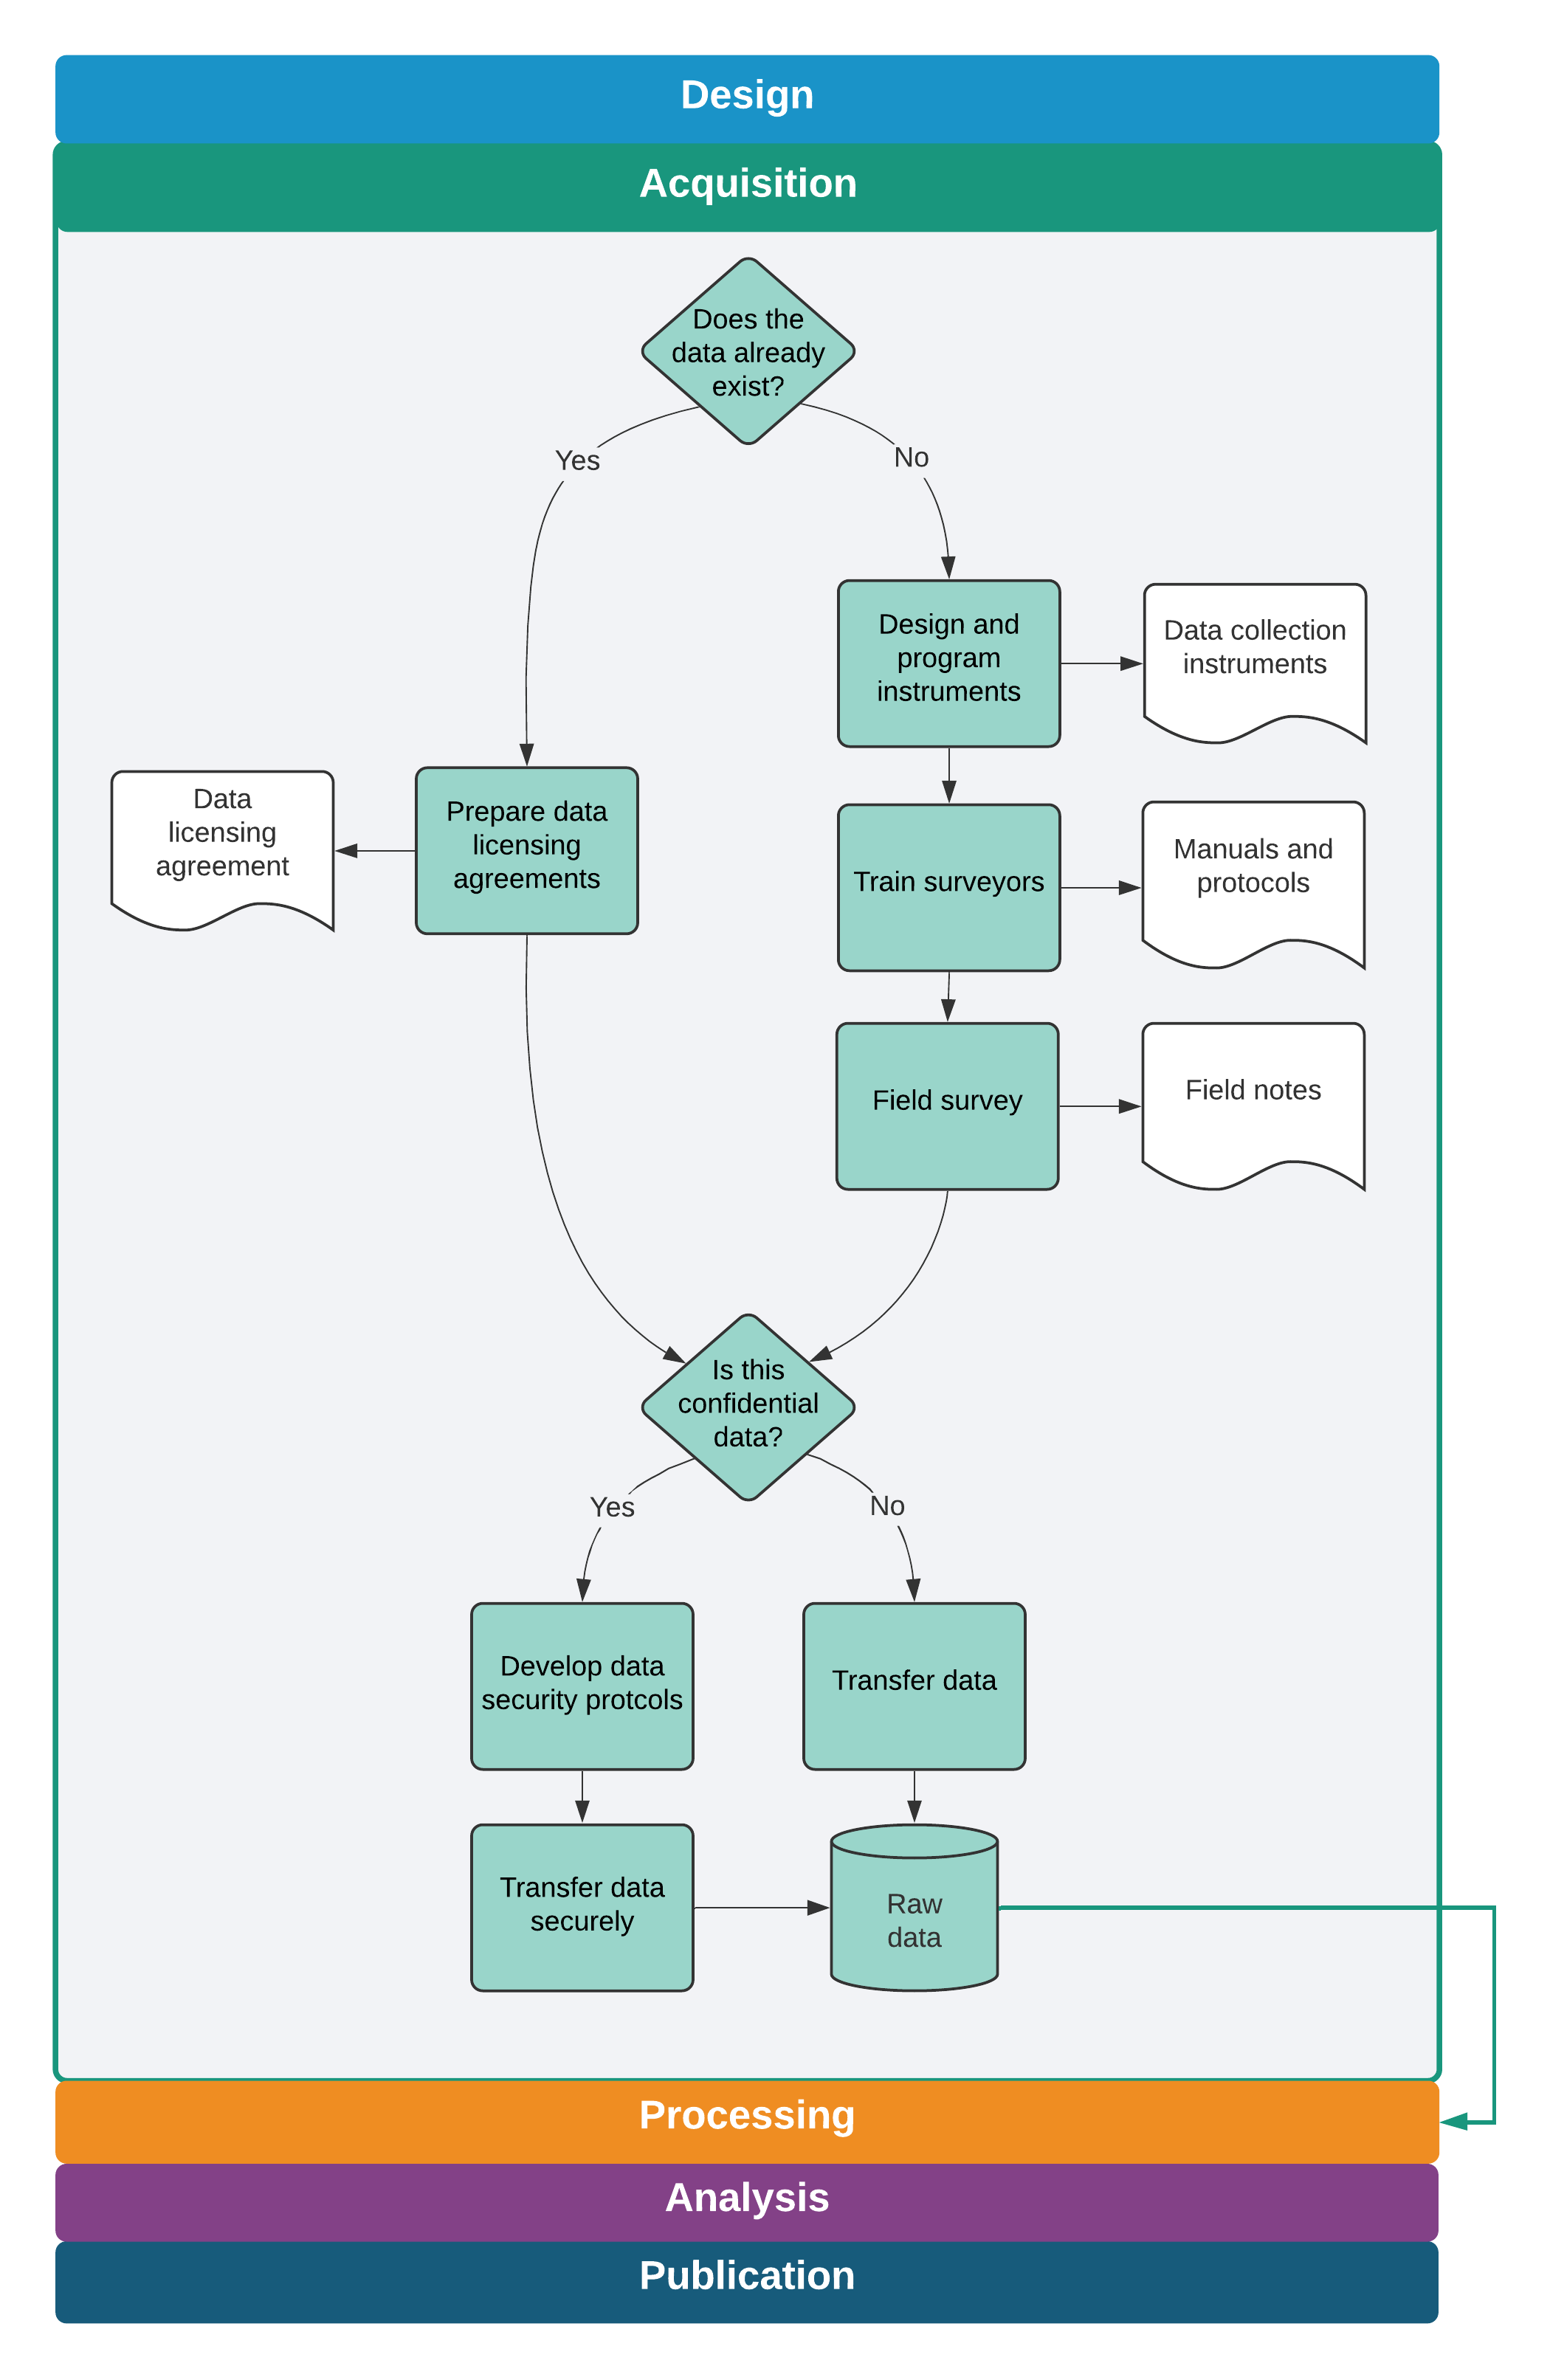
\includegraphics[width=1.5\linewidth]{diagrams/Acquisition}
	\end{figure}
\end{fullwidth}




%----------------------------------------------------------------------------------------
%	CHAPTER 5
%----------------------------------------------------------------------------------------

\chapter{Chapter 5: Cleaning and processing research data}
\label{ch:5}

%------------------------------------------------

\begin{fullwidth}

% What is data cleaning
Raw data files may be received in a variety of formats,
and are often not immediately suited for use with statistical software.
This chapter describes the workflow of preparing newly-acquired data for analysis.
The tasks described in this chapter have many different names:
data cleaning, data munging, data wrangling.
But they all mean the same thing --
transforming raw data into a more convenient and less error prone format for your intended use.
This is the most time-consuming step of a project's data work,
particularly when primary data is involved;
it is also essential for data quality.
This chapter outlines the workflow our team developed to make the process efficient and transparent.
One key point of this chapter is that no changes are made to the contents of data at this point.
We consider creating new variables, imputing values and correcting outliers
to be research decisions, and will discuss those in the next chapter.
Therefore, the clean dataset,
which is the main output from the workflow discussed in this chapter,
contains almost exactly the same information as the raw data,
but in a format that is ready for use with statistical software.

% Chapter overview
This chapter describes the various tasks involved in making newly-acquired data ready for analysis.
The first section will show how to make your data \textit{tidy}.
This means adjusting how the dataset is organized
until the relationship between its rows and columns is well-defined.
The second section describes quality assurance checks,
which are necessary to verify the accuracy of your data.
After that, identifying information is typically no longer needed;
therefore the third section outlines steps to remove direct identifiers.
Finally, the last section discusses how to examine each variable in your dataset and
make sure that it is as well documented and as easy to use as possible.
One important thing to take note is that all these tasks are implemented through code,
and resulting datasets are saved in new files that can be reproduced by running this code.
The raw data files are kept exactly as they were acquired,
and no changes are made directly to them.

\end{fullwidth}

%------------------------------------------------


\section{Identifying the identifier(s)}

% Intro
The very first step in creating an analysis-friendly dataset
is understanding the data acquired,
and using this understanding to translate the data into an intuitive format.
This section discusses what steps may be needed to make sure that each row
in your \textbf{data tables}\sidenote{\textbf{Data table:}
	data that is structured into rows and columns.
	Also called \textit{tabular datasets} or \textit{rectangular data}.
	Examples of non-rectangular data are written text,
	NoSQL and graph databases, or files such as images.}
represents one observation.
This may seem trivial, but should not be taken for granted.
This section will also present what we call a \textit{tidy} data format,
which is, in our experience, the ideal format to handle tabular data.

%------------------------------------------------------------------------------
\subsection{Unique identifiers}

% Uniquely and fully identifying variable
An important step before starting to tidy a dataset is
to understand the \textbf{unit of observation}\sidenote{
	\textbf{Unit of observation:} the unit described by the data.
	In a data table, it is ideally what each row represents. \url{
		https://dimewiki.worldbank.org/wiki/Unit\_of\_Observation}}
and find out which variable or set of variables is the \textbf{unique identifier}\sidenote{\url{
		https://dimewiki.worldbank.org/ID\_Variable\_Properties}}
for each observation.
Ensuring that observations are uniquely and fully identified
is arguably the most important step in data cleaning.
It may be the case that the variables expected to uniquely identify
the raw data contain either missing or duplicate values.\sidenote{
	Throughout this book, we use the expression \textbf{raw data}
	to refer to data in the state it was originally received by the research team.
	This applies to data acquired from partners as well as
	original data  collected by the research team.
}
It is also possible for a raw dataset to not include an unique identifier,
or for the identifier to involve a long string
that is difficult to work with, such as a person's name.
In such cases, cleaning begins by either carefully creating a variable
that uniquely identifies the data,
or merging the ID variable from the master dataset
using other identifying information.
Note that while digital survey tools create unique identifiers for each data submission,
that is not the same as having a unique ID variable for each observation in the sample,
as there can be multiple submissions for the same observation.

As discussed in Chapter 3,
the unique identifier will be used to link observations in this dataset
to data in other data sources according to the \textbf{data linkage table},\sidenote{
	\textcolor{red}{\url{https://dimewiki.worldbank.org/ LINK TO WIKI}}}
and all observation must be listed in the \textbf{master dataset}.\sidenote{
	\url{https://dimewiki.worldbank.org/Master\_Data\_Set}}
Part of the process of understanding the level of observation in a dataset
and finding or creating its unique identifier is to
make sure that each observation is represented in the master dataset by a unique ID value.
If you encounter any observations that are not listed in the master dataset,
you should assign them a unique ID and add them to the master dataset.
Always convince yourself beyond reasonable doubt that the new observation
is indeed a new observation,
and not one that is already listed, only with a different ID value.

DIME Analytics created an automated workflow to identify, correct and document
occurrences of duplicated entries in the unique identifier using
\texttt{ieduplicates} and \texttt{iecompdup},
two Stata commands included in the \texttt{iefieldkit}
package\index{iefieldkit}.\sidenote{\url{https://dimewiki.worldbank.org/iefieldkit}}
One advantage of using \texttt{ieduplicates}\sidenote{\url{
		https://dimewiki.worldbank.org/wiki/ieduplicates}}
to correct duplicated entries is that it creates \textit{duplicates reports}
which records each corrections made and documents the reason for it.
Even if you are not using this command,
it is important to keep a record of all cases of duplicated IDs encountered
 and how they were resolved.

%-------------------------------------------------------------------------------
\subsection{Tidying raw data}

Though raw data can be acquired in all shapes and sizes,
it is most commonly received as one or multiple data tables.
These data tables can organize information in multiple ways,
and not all of them result in easy-to-handle datasets.
Fortunately, a vast literature of database management has identified the format
that makes interacting with the data as easy as it can be.
In database management this is called \textit{normalization},
but when applied to statistics, we call data in such format \textbf{tidy}.
A data table is tidy when each column represents one variable,\sidenote{
  \textbf{Variable:} the collection of all data points
	that measure the same attribute.}
each row represents one observation,
and all variables in it have the same unit of observation.
Every other format is \textit{untidy}.
This may seem trivial, but raw data,
and raw survey data in particular,
is rarely received in a tidy format.
To contribute to the confusion,
in Stata each column is called a ``variable'',
and each row an ``observation'',
even though these do not necessarily equate.

Every untidy dataset is untidy in its own way,
but the most common case of untidy raw data encountered in development research
is a dataset with multiple units of observations stored in the same data table.
Take, for example, a household survey that includes household-level questions,
as well as a household member roster.
Such raw datasets usually consists of a single data table
where questions from the household member roster are saved in different columns,
one for each member, with a corresponding member suffix,
and household-level questions are represented by one column each.
When your rows include multiple nested observational units,
then the identifying variable does not identify all observations on that row,
as there is more than one unit of observation on the same row.
Survey data containing nested units of observation is typically
imported from survey platforms in \textbf{wide format}.\sidenote{\textbf{Wide data:}
	a data table where a single variable is divided into multiple columns,
	for example one for each individual in a household.
}
Wide format data could have, for instance,
one column for a household-level variable (for example \texttt{ownsfridge}),
and a few columns for household member-level variables (for example \texttt{sex\_1}, \texttt{sex\_2}).
Raw data is often saved in this format because it's the most efficient way to transfer it:
adding different levels of observation into the same data table
allows for data to be transferred in a single file.
However, this leads to the widespread practice of interacting with data in wide format,
although doing so is often inefficient and error-prone.

To understand how dealing with wide data can be complicated,
imagine you need to calculate the share of women
in each household using the household level data described above.
In a wide data table you will either have to first create variables counting
the number of women and the total number of household members,
and then calculate the share,
or you will have to transform the data to a different format.
In a tidy data table, however, where each row is a household member,
you can easily aggregate the share of women by household,
without additional steps,
and then merge the result to the household-level data tables.
Tidy data tables are also easier to clean,
as each attribute only needs to be checked once,
and each column corresponds directly to one question in the questionnaire.
Finally, as you will see in Chapter 6,
summary statistics and distributions are much simpler
to generate from tidy data tables.

As mentioned earlier, there are unlimited ways for data to be untidy;
wide format is only one of those ways.
Another example is a data table containing both information on transactions
and on the firms involved in each transaction.
In this case, the firm-level information will be repeated
for all transactions a given firm was involved in.
Analyzing data in this format would give more weight
to firms that conducted more transactions,
which may not be consistent with the research design.

The basic process behind tidying a data table is simple:
first, identify all the variables that were measured at the same level of observation;
second, create separate data tables for each level of observation;
and third, reshape\sidenote{\textbf{Reshape:}
	transform a data table in such a way that the unit of observation represented by a row changes.}
the data and remove duplicated rows
until each data table is uniquely and fully identified by the identifying variable
that corresponds to its unit of observation.
Reshaping data tables is the most intricate task in data cleaning;
you should be very familiar with commands such as
\texttt{reshape} in Stata and \texttt{pivot} in R.
You must be sure that identifying variables are consistent across data tables,
so they can always be linked.
Reshaping is the type of transformation we referred to
in the example of how you calculate
the share of women in a wide data set.
The important difference is that
in a tidy workflow,
instead of transforming the data for each operation,
this transformation is done once for all data during cleaning,
making all subsequent operations much easier.

In the earlier household survey example,
household-level variables will be stored in one tidy data table,
and household-member variables are reshaped
and stored in a separate, member-level, tidy data table,
which also contains the household ID for each individual.
The household ID is intentionally duplicated in the household members data table
to allow one or several household members to be linked to the same household data.
The unique identifier for the household member-level data data will be
either a single household member ID or
a combination of household ID and household member ID.
In the transaction data example,
the result of the tidying process would be one transaction-level data table,
containing variables indicating the ID of all firms involved;
and one firm-level data table with a single entry for each firm.
Then, firm-level analysis is easily done
by calculating appropriate statistics in the transactions data table
(in Stata, often through \texttt{collapse})
and then merging or joining those results to the firms data table.

In a tidy workflow, your clean dataset is a set of one or more tidy data tables.
In both examples above, your clean dataset is made up of two tidy data tables.
There must be a clear way to connect each
tidy data table to a master dataset,
and thereby also to all other datasets.
To implement this, you need to decide which data table is the main data table;
that data table's unit of observation will be
the main unit of observation of your dataset.
The main unit of observation must directly correspond to a master dataset,
and be listed in the data linkage table.
All other data tables in your dataset must have
an unambiguous way to merge with the main data table.
This way, it will be possible to link
all data points in all your project's datasets to each other.
We recommend that you save your datasets as a folder,
in which the main data table shares the same name as the folder,
and the name of all other data tables start with the same name,
but are suffixed with the unit of observation for that data table.

In the household dataset example,
the household-level data table would be the main table.
This means that there must be a master dataset for households.
(You may have a master dataset for household members as well
if you think it is important for your research,
but it is not strictly required).
The household data set would then be stored in a folder called,
for example, \texttt{baseline-hh-survey/}.
In that folder you would save both
the household-level data table with the same name as the folder,
for example \texttt{baseline-hh-survey.csv},
and the household member-level data named on the same format but with a suffix,
for example \texttt{baseline-hh-survey-hhmember.csv}.

The tidying process gets more complex as the number of nested groups increases.
That means the steps of identifying the unit of observation of each variable
and reshaping the separated data tables need to be repeated multiple times.
However, the more nested groups a dataset includes,
the more efficient it is to deal with tidy data as compared to untidy.
Cleaning and analyzing wide datasets, in particular,
is a repetitive and error-prone process.

The next step of data cleaning, data quality monitoring,
may involve comparing different units of observation.
Aggregating sub-units to compare to a higher unit is much easier with tidy data,
which is why we suggest tidying data as the first step in the cleaning workflow.
If you are conducting primary data collection,
you can start preparing or coding the data tidying even before the data is acquired,
since you will know in advance the exact format in which the data will be received.
In the case of survey data,
tidying datasets will guarantee a one-to-one correspondence
between questions in the questionnaire and columns in the data.
Preparing the data for analysis, the last task in this chapter,
is much simpler when that is the case.

%------------------------------------------------
\section{Data quality assurance}

% Intro
Whether you are acquiring data from a partner or collecting it directly,
it is important to make sure that data faithfully reflects ground realities.
You should carefully examine and clean any data you are about to use.
When reviewing raw data, you will inevitably encounter data entry mistakes,
such as typos and inconsistent values.
Data quality assurance requires a combination of real-time data checks
and back-checks or validation audits, which often means tracking down
the people whose information is included in the dataset.

\subsection{Implementing high-frequency quality checks}

% What are HFCs
A key advantage of continuous electronic data ingestion methods,
as compared to traditional paper surveys and one-time data dumps,
is the ability to access and analyze the data acquisition process is ongoing.
Data issues can then be identified and resolved in real-time.
Designing systematic data checks and running them routinely throughout data intake
simplifies monitoring and improves data quality.
To prepare for data acquisition,
the research team should develop a \textbf{data quality assurance plan}\sidenote{
	\url{https://dimewiki.worldbank.org/Data\_Quality\_Assurance\_Plan}}.
While data is being acquired,
a research assistant should work closely with the field team or data licensing partner
to ensure that the data is flowing as expected,
and to set up and perform \textbf{high-frequency checks (HFCs)} with the incoming data.

% Why they should be made in real-time
High-frequency checks should carefully inspect key treatment and outcome variables
to ensure that the data quality of core study variables is uniformly high,
and that additional effort is centered where it is most important.
Data quality checks should be run every time data is received
to flag irregularities in the aquisition progress, in sample completeness, or in response quality.
The faster issues are identified, the more likely they are to be solved.
\texttt{ipacheck}\sidenote{
	\url{https://github.com/PovertyAction/high-frequency-checks/wiki}}
is a very useful Stata command that automates some of these tasks,
regardless of the data source.

% Completeness
It is important to check continuously that the observations received match the intended sample.
In surveys, electronic survey software often provides case management features
through which sampled units are directly assigned to individual enumerators.
For data received from partners, such as administrative data,
this may be harder to validate.
In these cases, cross-referencing with other data sources can help to ensure completeness.
It is often the case that raw data includes duplicate or missing entries,
which may occur due to typos, failed submissions to data servers,
or other mistakes.\sidenote{
	\url{https://dimewiki.worldbank.org/Duplicates_and_Survey_Logs}}
Issues with data transmission often result in missing observations,
particularly when large datasets are being transferred,
or when data is being collected in locations with limited internet connection.
Keeping a record of what data was submitted,
and comparing it to the data received as soon as transmission is complete
reduces the risk of noticing that data is missing when it is no longer possible to recover it.

% match to sample
Once data completeness is confirmed,
observed units must be validated against the expected sample:
this is as straightforward as merging the sample list
with the data received and checking for mismatches.
Reporting errors and duplicate observations in real time allows for efficient corrections.
\texttt{ieduplicates}\sidenote{
	\url{https://dimewiki.worldbank.org/ieduplicates}}
provides a workflow for resolving duplicate entries with the data provider.
For surveys, it is also important to track data collection progress to  monitor attrition,
so that it is clear early on if a change in protocols or additional tracking will be needed.
Remember to also check survey completion rates
and sample compliance by surveyors and survey teams,
and compare data missingness across administrative regions,
to identify any clusters that may be providing data of suspect quality.

% Consistency
High frequency checks should also include checks of response quality and consistency.
For example, whether the values for each variable fall within the expected range and
the answers provided by the same household are consistent across all survey modules.\sidenote{
	\url{https://dimewiki.worldbank.org/Monitoring_Data_Quality}}
Electronic survey and data entry software often incorporate many quality control features,
such as range restrictions and logical flows.
Data received from systems that do not include such controls should be checked more carefully.
Response consistency should be checked across all datasets, as this is much harder to automate.
Consistency checks are project specific, so it is difficult to provide general guidance.
A detailed knowledge of the variables in the dataset and a careful examination of the analysis plan
is the best way to prepare.
Analysis of metadata and paradata can also useful in assessing data quality.
For example, electronic survey software generates
automatically collected timestamps and trace histories,
showing when data was submitted, how long enumerators spent on each question,
and how man times answers were changed before or after the data was submitted.

% Following up on flagged issues
High-frequency checks will only improve data quality
if the issues they catch are communicated to the data provider
and corrections are documented and applied to the data.
There are lots of ways to do this;
what's most important is to find a way to create actionable information for your team.
\texttt{ipacheck}, for example, generates a spreadsheet with flagged errors;
these can be sent directly to the data collection teams.
Many teams choose other formats to display results,
such as online dashboards created by custom scripts.
It is also possible to automate communication of errors to the field team
by adding scripts to link the HFCs with a messaging platform.
Any of these solutions are possible:
what works best for your team will depend on such factors as
cellular networks in field work areas, whether field supervisors have access to laptops,
internet speed, and coding skills of the team preparing the HFC workflows.

\subsection{Conducting back-checks and data validation}

% Conducting back-checks
Careful validation of data is essential for high-quality original data.
While we cannot control natural measurement error,
which comes from variation in the realization of key outcomes,
there is often an opportunity to reduce error arising from inaccuracies in the data generation process.
\textbf{Back-checks}\sidenote{\url{https://dimewiki.worldbank.org/Back\_Checks}} and
other validation audits help ensure that data is not falsified, incomplete, or otherwise suspect.
For survey data, this can also be a means to ensure that all field protocols are followed.
For back-checks and validation audits, a random subset of observations is selected,
and a subset of information from the full survey is
verified through a brief targeted survey with the original respondent
or a cross-referenced dataset from another source (if the original data is not a field survey).
Design of the back-checks or validations follows the same survey design
principles discussed above: you should use the analysis plan
or list of key outcomes to establish which subset of variables to prioritize,
and similarly focus on errors that would be major flags for poor quality data.

% How to implement back-checks
Real-time access to the data massively increases the potential utility of validation,
and both simplifies and improves the rigor of the associated workflows.
You can use the raw data to draw the back-check or validation sample;
this ensures that the validation is correctly apportioned across observations.
As soon as high frequency checks are complete,
the validation data can be tested against
the original data to identify areas of concern in real-time.
The \texttt{bcstats} command is a useful tool for analyzing back-check data in Stata.\sidenote{
	\url{https://ideas.repec.org/c/boc/bocode/s458173.html}}
Some electronic surveys surveys also provide a unique opportunity
to do audits through audio recordings of the interview,
typically short recordings triggered at random throughout the questionnaire.
\textbf{Audio audits}\sidenote{\url{https://dimewiki.worldbank.org/Random\_Audio\_Audits}}
are a useful means to assess whether enumerators are conducting interviews as expected.
Do note, however, that audio audits must be included in the informed consent for the respondents,
and the recordings will need to be assessed by specially trained staff.


\section{De-identifying research data}

When implementing the steps discussed up to this point,
you are likely to handle confidential data.
Effective data quality monitoring
frequently requires you to identify the individual observations in your dataset,
and the people or other entities who provided the information.
Using identified data allows you to quickly follow up on and resolve identified issues.
Handling confidential data such as \textbf{personally-identifying information}\index{
	personally-identifying information}
requires a secure environment and, typically, decryption.
De-identifying the data will allow you to simplify that workflow,
and will also reduces the risk of harmful leaks.
This section describes how to de-identify data in order to share it with a wider audience.

\subsection{Protecting privacy as a researcher}

% Dealing with human subjects
Most development data involves human subjects.\sidenote{
	\url{https://dimewiki.worldbank.org/Human\_Subjects\_Approval}}
\index{human subjects}
As a researcher, you may have access to personal information about your subjects:
where they live, how much income they have,
whether they have committed or been victims of crimes,
their names, their national identity numbers, and other sensitive data.
There are strict requirements for safely storing and handling personally-identifying data,
and it is the responsibility of the research team to satisfy these requirements.\sidenote{
	\url{https://dimewiki.worldbank.org/Research\_Ethics}}
Everyone working with human subjects research should participate in an ethics training;
Protecting Human Research Participants\sidenote{
	\url{https://phrptraining.com}}
and the CITI Program;\sidenote{
	\url{https://about.citiprogram.org/en/series/human-subjects-research-hsr}}
are common options.
A plan for secure data handling is typically also required for IRB approval.

% Options for dealing with PII data: only collect it if extremely necessary, encrypt it, restrict access, de-identify it
The best way to avoid risk is to minimize interactions with PII as much as possible.
First, only collect personally-identifying information that is strictly necessary for the research.
Second, avoid the proliferation of copies of identified data.
There should never be more than one copy of the raw identified dataset in the working project folder,
and it must always be encrypted.
Third, de-identify the data as early as possible in the workflow.
Even within the research team,
access to the identified data should be limited to team members who require it for their specific tasks.
Data analysis that requires identifying information is rare
and in most cases can be avoided by properly linking masked identifiers to research information
such as treatment statuses and weights, then removing unmasked identifiers.

% De-identification vs anonymization
Once data is acquired and the data quality checks described above are completed,
the next task is typically to \textbf{de-identify} the data,
by removing or masking all personally-identifying variables.\sidenote{
	\url{https://dimewiki.worldbank.org/De-identification}}
\index{de-identification}
Note that it is in practice impossible to \textbf{anonymize} data.
There is always some statistical chance that an individual's identity
will be re-linked to the stored data
-- even if that data has had all directly identifying information removed --
by using some other data that becomes identifying when integrated.
For this reason, we typically recommend de-identification in two stages.
The \textbf{initial de-identification} process,
performed as soon as data is acquired, strips the data of direct identifiers,
to create a working de-identified dataset that
can be shared \textit{within the research team} without the need for encryption.
The \textbf{final de-identification} process,
performed before data is publicly released, involves
careful consideration of the trade-offs between
risk of identifying individuals and the utility of the data,
and typically requires the removal of a further level of indirect identifiers.\sidenote{
	\url{https://sdcpractice.readthedocs.io/en/latest/SDC\_intro.html\#need-for-sdc}}
The rest of this section describes how to implement
both the initial and the final de-identification processes.


\subsection{De-identification in practice}

% Initial de-identification
Initial de-identification reduces risk and simplifies workflows.
Once you create a de-identified version of the dataset,
you no longer need to interact directly with the encrypted data.
Note that if the data tidying resulted in multiple raw data tables,
each will need to be de-identified separately, but
the workflow will be the same for all of them.

During the initial round of de-identification,
datasets must be stripped of personally identifying information.\sidenote{
	\url{https://dimewiki.worldbank.org/De-identification}}
To do so, you will need to identify all variables that contain
such information.\sidenote{\url{
		https://www.povertyactionlab.org/sites/default/files/resources/J-PAL-guide-to-deidentifying-data.pdf}}
For data collection, where the research team designs the survey instrument,
flagging all potentially identifying variables at questionnaire design stage
simplifies the initial de-identification process.
If you did not do that, or you received original data by another means,
there are a few tools to help flag variables with personally-identifying data.
JPAL's \texttt{PII-scan} and
IPA's \texttt{PII\_detection},\sidenote{
	\url{https://github.com/PovertyAction/PII\_detection}}
scan variable names and labels for common string patterns associated with identifying information.\sidenote{
	\url{https://github.com/J-PAL/PII-Scan}}
The World Bank's \texttt{sdcMicro}
lists variables that uniquely identify observations,
but its more refined method and
higher processing capacity requirement make it better suited for final de-identification.\sidenote{
	\url{https://sdctools.github.io/sdcMicro/articles/sdcMicro.html}}
The \texttt{iefieldkit} command \texttt{iecodebook}
lists all variables in a dataset and exports an Excel sheet
where you can easily select which variables to keep or drop.\sidenote{
	\url{https://dimewiki.worldbank.org/Iecodebook}}

% Initial de-identification in practice
Once you have a list of variables that contain confidential information,
assess them against the analysis plan and first ask yourself for each variable:
\textit{will this variable be needed for the analysis?}
If not, the variable should be dropped.
Don't be afraid to drop too many variables the first time,
as you can always go back and extract additional variables from the raw data,
but you cannot go back in time and drop a PII variable that was leaked.

For each confidential variable that is needed in the analysis, ask yourself:
\textit{can I encode or otherwise construct a variable that masks the confidential component, and
	then drop this variable?}
This is typically the case for most identifying information.
If the answer to either of the two questions above is yes,
all you need to do is write a script to drop the variables that are not required for analysis,
encode or otherwise mask those that are required,
and save a working version of the data.
For example:
after constructing measures of distance or area,
drop the specific geolocations in the data;
after constructing and verifying numeric identifiers in
a social network module, drop all names.
If confidential information is strictly required for the analysis and cannot be
masked or encoded,
it will be necessary to keep at least a subset of the data encrypted through
the data analysis process.

% Final de-identification: sdcMicro
After initial de-identification is complete,
your dataset will consist of one or multiple tidy,
de-identified data tables.
This is the dataset that you will interact with
during the remaining tasks described in this chapter.
Initial de-identification should not affect the usability of the data.
Note that access to the initially de-identified data
should still be restricted to the research team only,
as indirect identifiers may still present a high risk if disclosure.
It is common, and even desirable, for teams to make data publicly available
once the tasks discussed in this chapter are concluded.
This will allow other researchers to conduct additional analysis and to reproduce your finding.
Before that can be done, however,
you should further consider whether your data can be re-identified,
in a process we call \textbf{final de-identification},
which will be discussed in more detail in Chapter 7.


\section{Preparing data for analysis}

% What is data cleaning
The last step in the data cleaning process involves
making the dataset easy to use and understand, and
carefully examining each variable to document distributions
and identify patterns that may bias the analysis.
The resulting dataset will contain only the variables collected in the field, and
no modifications to data points will be made,
except for corrections of mistaken entries.
You may have more data tables in your dataset now then originally received,
and they may have a different \textit{format},
but the information contained is still the same.
Apart from the \textbf{cleaned dataset} (or datasets) itself,
cleaning will also yield extensive documentation describing it.

% Section overview
Data cleaning yields in-depth understanding of the contents and structure of your data.
This knowledge will be key to correctly constructing and analyzing final indicators.
Do not rush through this step!
It is common for cleaning to be the most time-consuming task in a project.
In this section, we introduce some concepts and tools to make it more efficient and productive.
The section is separated into three subtopics:
exploring the data, making corrections, and recoding and annotating.
They are separated here because they are different in nature,
and should be kept separated in your code.
In practice, however, they may all done at the same time.


\subsection{Exploring the data}

% What to look for when exploring the data
The first time you interact with the data is during quality checks.
However, these checks are are usually time-sensitive,
and there may not be time to explore the data at length.
During data cleaning, on the other hand,
you will need to inspect each variable closely.
Use tabulations, summary statistics, histograms and density plots to understand the structure of data,
and look for patterns or irregularities.
Think critically about what you see:
are the values shown consistent with the information the variable represents?
How do distributions look?
Are there any outliers or missing values?
Could distributional patterns be caused by data entry errors,
particularly in primary data?
Are related variables consistent with each other?

% Document patterns rather than fix them
At this point, it is more important to document your findings
than to directly address any irregularities found.
There is a very limited set of changes that should be made to the raw data during cleaning.
They are described in the next two sections,
and are usually applied to each variable as you examine it.
Most of the transformations that result in new variables
will be done during \textbf{construction}, a process discussed in the next chapter.
For now, focus on creating a record of what you observe,
and extensively documenting the data being explored.
You will use this documentation when discussing with your team
how to address irregularities once you get to the construction stage.
This material will also be valuable during exploratory data analysis.

\subsection{Correcting data points}

% Correct or not correct
As mentioned earlier,
corrections to issues identified during data quality monitoring are
the only changes done to individual data points during the data cleaning stage.
However, there is a lot of discussion about whether one should modify such data points at all.
Some argue that follow-ups to the issues identified are costly and add limited value.
Since it is not possible to check each and every possible data entry error,
doing so can create a false sense of security from issues identified on a few main variables.
Additionally, manually-inspected data may suffer from considerable inspector variability.
In many cases, the main purpose of data quality checks
is to detect fraud and identify problems with data collection protocols.
On the other hand, there is also an argument to be made
against keeping clear typing errors or not correcting missing values.
We recommend correcting any entries that are clearly identified as errors.
However, there is a great deal of subjectivity involved in deciding
which cases fall into this category.
This, as many others decisions that fall upon research teams,
is more of an art than a science, and
we will not attempt to make general recommendations.
Making this such decisions involve deep knowledge of the data and
the particular circumstances or each research project.


% Documentation
Whether you decide to modify your data or not,
you must keep a careful record of all issues that you identify.
If no data points are modified,
it may still be helpful to add flags to observations containing
potentially problematic values,
so you can verify how they affect results during analysis.
If your team decides to follow up on and correct these issues,
the follow-up process must also be thoroughly documented.
Be very careful not to include confidential information in documentation that is not securely stored,
or that you intend to release as part of a replication package or data publication.
Finally, remember not to make changes directly to the raw data.
Instead, any corrections must be done as part of data cleaning,
applied through code, and saved to a new dataset.

\subsection{Recoding and annotating data}

% Why recoding and annotating data are important
The cleaned dataset is the starting point of data analysis.
It will be extensively manipulated to construct analysis indicators,
so it is important for it to be easily processed by statistical software.
To make the analysis process smoother,
anyone opening this dataset for the first time should have all the information needed to interact with it,
even if they were not involved in the acquisition or cleaning process.
This will save them time going back and forth between the dataset and its accompanying documentation.

% Encoding variables
Often times, datasets are not imported into statistical software in the most efficient format.
The most common example is string (text) variables:
categorical variables and open-ended responses are often read as strings.
However, variables in this format cannot be used for quantitative analysis.
Therefore, categorical variables must be transformed into other formats,
such as \texttt{factors} in R and \texttt{labeled integers}\sidenote{\url{
		https://dimewiki.worldbank.org/wiki/Data\_Cleaning\#Value\_Labels}} in Stata.
Additionally, open-ended responses stored as strings usually have a high risk of including identifying information,
so cleaning them requires extra attention.
The choice names in categorical variables
(called \textit{value labels} in Stata and \textit{levels} in R)
should be accurate, concise,
and directly linked to the data collection instrument.
Adding choice names to categorical variables
makes it easier to understand your data as you explore it,
and thus reduces the risk of small errors making their way through into the analysis stage.

% Recoding missing values
In survey data, it is common for non-responses such as ``Don't know'' and ``Declined to answer''
to be represented by arbitrary survey codes.
The presence of these values could bias your analysis,
since they don't represent actual observations of an attribute.
They need to be turned into \textit{missing values}.
However, the fact that a respondent didn't know how to answer a question is also useful information
that would be lost by simply omitting all information.
In Stata, this information can be elegantly conserved using extended missing values.\sidenote{
	\url{https://dimewiki.worldbank.org/Data\_Cleaning\#Survey\_Codes\_and\_Missing\_Values}}

% Labeling variables
We recommend that the cleaned dataset be kept as similar to the raw data as possible.
This is particularly important regarding variable names:
keeping them consistent with the raw data makes data processing and construction more transparent.
Unfortunately, not all variable names are informative.
In such cases, one important piece of documentation
 makes the data easier to handle: the variable dictionary.
When a data collection instrument (for example a questionnaire) is available,
it is often the best dictionary one could ask for.
But even in these cases, going back and forth between files can be inefficient,
so annotating variables in a dataset is extremely useful.
In Stata, \textit{variable labels}\sidenote{\url{
	https://dimewiki.worldbank.org/wiki/Data\_Cleaning\#Variable\_Labels}}
must always be present in a cleaned dataset.
They should include a short and clear description of the variable.
A lengthier description, that may include, for example,
the exact wording of a question, may be added through \textit{variable notes}.
In R, it is less common to use variable labels,
and a separate dataset with a variable dictionary is often preferred,
but \texttt{data frame attributes} can be used for the same purpose.

% Dropping irrelevant variables
Finally, any information that is not relevant for analysis may be removed from the dataset.
In primary data, it is common to collect information for quality monitoring purposes,
such as notes, duration fields and surveyor IDs.
Once you are past the quality monitoring phase,
these variables may be removed from your dataset.
In fact, to make the data easier to handle,
you may choose to start from a minimal set of variables,
and add new ones as you clean them.
To ensure the cleaned dataset file doesn't get too big to be handled,
use commands such as \texttt{compress} in Stata so the data
is always stored in the most efficient format.

% Cleaning tools: iecodebook, tidyverse
Although all these tasks are key to making the data easy to use,
implementing them can be quite repetitive and create convoluted scripts.
The \texttt{iecodebook} command suite, part of the \texttt{iefieldkit} Stata package,
is designed to make some of the most tedious components of this process more efficient.\sidenote{
	\url{https://dimewiki.worldbank.org/iecodebook}}\index{iecodebook}
It also creates a self-documenting workflow,
so your data cleaning documentation is created alongside that code,
with no extra steps.
As far as we know, currently there are no similar resources in R.
However, the \texttt{tidyverse}\sidenote{\url{https://www.tidyverse.org/}} packages
compose a consistent and useful grammar to perform the same tasks.

%--------------------------------------------------------------
\subsection{Documenting data cleaning}

Throughout the data cleaning process,
you will often need extensive inputs from the people responsible for data collection.
Sometimes this is your research team, but often it will be someone else.
It could be a survey team, the government ministry responsible for administrative data systems,
the technology firm that generated remote sensing data, etc.
Regardless of who originally collected the data,
you should acquire and organize all documentation of how the data was generated.\sidenote{
	\url{https://dimewiki.worldbank.org/Data\_Documentation}}
\index{Documentation}
What type of documentation that is available depends on how the data was collected.
For original data collection, this should include
field protocols, data collection manuals, survey instruments,
supervisor notes, and data quality monitoring reports.
For secondary data, you should try to get the same type of information,
but that is often not possible unless
the data source is a well managed data publication.
Independently of its exact composition,
the data documentation should be stored
alongside your data dictionary and codebooks.
You will probably need these files during analysis,
and they should be published along with the data,
so other researchers may use them for their analysis as well.

Once you have a cleaned,
de-identified dataset with one or several data tables,
and the documentation to support it,
you have created the first research output of your project: a dataset.
Chapter 7 will get into the details of data release.
For now, all you need to know is that your team
should consider submitting this dataset for publication,
or at least archiving and cataloguing,
even if it will remain embargoed for some time.
This will help you organize your files and create a backup of the data,
and some donors require that the data be filed as an intermediate step of the project.
However, the reason why you acquired and cleaned this data
was a research question.
Though data cleaning is typically the most time-consuming process in the data work,
the reason why it is done is preparing data to be analyzed.
In chapter 6, you will see what are the last few steps needed to finally run the
regressions originally specified in your analysis plan
and find an answer to your research question --
or perhaps to find out you now have even more questions.

%--------------------------------------------------------------


%----------------------------------------------------------------------------------------
%	CHAPTER 6
%----------------------------------------------------------------------------------------

\chapter{Chapter 6: Analyzing research data}
\label{ch:6}

%------------------------------------------------

\begin{fullwidth}

% Intro ----------------------------------------

% Motivation

The process of data analysis is typically
a back-and-forth discussion between people
with differing skill sets.
To effectively do this in a team environment,
data, code and outputs must be well-organized,
with a clear system for version control,
analysis scripts that can be run by all team members,
and creation of research outputs fully automated.
Putting in time upfront to structure the data analysis workflow
in this way pays substantial dividends throughout the process.
Transparently documenting research decisions made during data analysis
is essential for reproducible research.

% Chapter overview
In this chapter, we discuss the process of transforming
cleaned raw data into the final analysis dataset(s).
The suggested workflow starts from clean raw data
(the output of data cleaning, discussed in the previous chapter).
The first section covers variable construction:
transforming the raw data into economically meaningful indicators.
The second section discusses the analysis itself.
We do not offer instructions on how to conduct specific analyses,
as that is determined by research design,
and there are many excellent existing guides.
Rather, we discuss how to structure analysis code
so that it is easy to follow and understand,
for both the full research team members and a public audience.
The final section discusses ways to automate common outputs
so that your work is fully reproducible.

\end{fullwidth}

%------------------------------------------------

\section{Creating analysis datasets}

% What is construction
For this chapter, we assume you are starting from
one or multiple well-documented tidy\sidenote{\citet{hadley2017R}} datasets.
We also assume that these datasets
have gone through thorough quality checks
and incorporate any corrections needed.
The next step is to \textbf{construct}\sidenote{
	\textbf{Data construction}:
	The process of transforming cleaned data into analysis data by
	creating the derived indicators that will be analyzed.}
the variables that you will use for analysis;
that is, to transform the cleaned data into analysis-ready data.
It's possible the acquired data is ready for analysis,
but in most cases it needs to be prepared by integrating different datasets
and creating derived variables
(dummies, indices, and interactions, to name a few\sidenote{
  See \citet{adjognon2019reducing} for an example.}).
The derived indicators you will construct should be
planned during research design\index{research design};
the pre-analysis plan should serve as your guide
at this stage.\index{pre-analysis plan}
During construction, data will typically be
reshaped, merged, and aggregated to change the level of the data points
from the \textbf{unit of \textit{observation}} in the raw data
to the \textbf{unit of \textit{analysis}}.\sidenote{\url{
		https://dimewiki.worldbank.org/Unit\_of\_Observation}}\index{unit of observation}\index{unit of analysis}

% A project may require multiple purpose-built data sets
Each analysis dataset is built to answer an analysis question.
If the sub-samples and units of observation
vary for different pieces of the analysis,
you may need to create many purpose-built analysis datasets.\index{analysis datasets}
In such cases, it is not good practice
to try to create a single ``one-size-fits-all'' analysis dataset.
For a concrete example of what this means,
think of an agricultural intervention
that was randomized across villages
and only affected certain plots within each village.
The research team may want to
run household-level regressions on income,
test for plot-level productivity gains,
and check if village characteristics are balanced.
Having three separate datasets for each of these three pieces of analysis
will result in cleaner, more efficient, and less error-prone analytical code than if
you started from a single analysis dataset and repeatedly transformed it.

\subsection{Fitting construction into the data workflow}

% Why construction is separate from data cleaning
Construction follows data cleaning and
should be treated as a separate task for two reasons.
First, this helps to clearly differentiate error corrections
(necessary for all data uses)
from creation of analysis indicators
(necessary only for specific analyses).
Second, it helps to ensure that variable definitions are
consistent across datasets.
Construction can create many outputs combining many inputs,
and, unlike in data cleaning,
resulting datasets should be concise rather than exhaustive.
For example, take a project that has a baseline and an endline survey.
Unless the two data collection instruments are exactly the same,
which is preferable but often not the case,
the data cleaning for each of these rounds will require different steps,
and therefore will be done separately.
However, the analysis indicators must be constructed in the exact same way,
so they are comparable.
To do this, you will require at least two separate cleaning scripts,
and a unified construction script.
Maintaining one construction script guarantees that you will not
accidentally make changes to an indicator from one round
while forgetting to update the other.

% Why construction is separate from analysis
When we visualize the research workflow,
variable construction precedes data analysis,
as derivative variables need to be created before they are analyzed.
In practice, however, as you analyze the data,
it is often useful to revisit construction,
and explore different subsets of the same and other transformations of the data.
Even if construction and analysis are done concurrently,
you should always do the two in separate scripts.
If every script that creates a table starts by loading a dataset,
subsetting it, and manipulating variables,
any edits to construction need to be replicated in all scripts.
This increases the chances that at least one of them
will have a different sample or variable definition.
Doing all variable construction and data transformation
in a unified script, separate from the analysis code, helps
avoid this and ensures consistency across different outputs.

\subsection{Integrating different data sources}

% When merging is necessary and how to start thinking about it
To create the analysis dataset,
it is typically necessary to combine information
from different data sources.\sidenote{\url{
		https://dimewiki.worldbank.org/Data\_Integration}}
As discussed in Chapter 3,
this process should be documented
using \textbf{data flowcharts},\sidenote{
	\url{https://dimewiki.worldbank.org/Data\_Flow\_Charts}}
and different data sources should only be combined
in accordance with the data linkage table.\sidenote{
	\url{https://dimewiki.worldbank.org/wiki/Data\_Linkage\_Table}}
For example, you may merge administrative data with survey data
in order to include demographic information in your analysis,
or you may want to integrate geographic information
in order to include location-specific controls.
To understand how to perform such operations,
you will need to consider the unit of observation for each dataset,
and their respective identifying variables.
Merges are frequent and complex operations,
which makes them a common source of error.
Whichever statistical software you are using,
take the time to read through the help file of merge commands
and make sure you understand their options and outputs.\index{merging data}

% How to think about merges
When writing the code to implement merge operations,
a few steps can help avoid mistakes.
First, before writing code to combine the datasets,
write pseudocode to understand which observations you expect to be
matched or not, and why.
When possible, determine exactly which and how many
matched and unmatched observations should result from the merge.
The best tool you have to understand this is
the three components of the data map discussed in chapter 3.
Second, think carefully about whether you want to keep matched and unmatched observations,
or only specific matching outcomes (e.g. to create a balanced panel),
and add that to the pseudocode as well.
Finally, run the code to merge the datasets,
and compare outcome to your expectations.
Add comments to explain any exceptions,
and make it so the code will return an error in case unexpected results show up in future runs.

% Common mistakes
To avoid unintentional changes to your data,
pay close attention to merge results.
Two issues to pay extra attention to are missing values and dropped observations.
Make sure to read about how each command treats missing observations:
are unmatched observations dropped, or are they kept with missing values?
Whenever possible, add automated checks in the script that throw an error message
if the result is different than what you expect,
or you may not changes in the outcome running large portions of code.
Document changes in the number of observations in your comments,
and explain why they are happening.
If your are subsetting your data by keeping only matched observations,
write down the reason why the observation differ across datasets,
as well as why you are only interested in those that matched.
The same applies when you are adding new observations from the merged dataset.

% Data integration
Some merges of data with different units of observation
are more conceptually complex.
Examples include: overlaying road location data with household data,
using a spatial match; combining school administrative data, such as attendance records and test scores,
with student demographic characteristics from a survey;
or linking a dataset of infrastructure access points, such as water pumps or schools,
with a dataset of household locations.
In these cases, a key part of the research contribution is figuring out
a useful way to combine the datasets.
Since the conceptual constructs that link observations from the two data sources
are important and can take many possible forms,
it is especially important for the data integration to not be treated mechanically,
and to be extensively documented, separately from other data construction tasks.


\subsection{Creating analysis variables}

% Main points to keep in mind for new variables
Once you have assembled variables from different sources into a single working dataset
with the right raw information and observations,
it's time to create the derived indicators of interest for analysis.\index{analysis variables}
Before constructing new indicators,
you must check and double-check units, scales, and value assignments of each variable that will be used.
This is when you will use the knowledge
of the data and the documentation developed during cleaning the most.
First, check that all categorical variables have the same value assignment,
such that labels and levels have the same correspondence across variables that use the same options.
For example, it's possible that in one question \texttt{0} means ``no'' and \texttt{1} means ``yes'',
while in another one the same answers were coded as \texttt{1} and \texttt{2}.\index{binary variables}
(We recommend coding binary questions as either \texttt{1} and \texttt{0} or \texttt{TRUE} and \texttt{FALSE},
so they can be used numerically as frequencies in means and as dummies in regressions.
This often implies re-expressing categorical variables like \texttt{gender} as binary variables like \texttt{woman}.)
Second, make sure that any numeric variables you are comparing
are converted to the same scale or unit of measure:
you cannot add one hectare and two acres and get a meaningful number.
New variables should be assigned functional names,
and the dataset ordered such that related variables are together.
Adding notes to each variable will make your dataset more user-friendly.

% Dealing with outliers and missing values
At this point, you will also need to decide
how to handle any outliers or unusual values identified during data cleaning.
How to treat outliers is a research question.\sidenote{
	\url{https://dimewiki.worldbank.org/Variable_Construction\#Dealing_with_outliers}}\index{outliers}
There are multiple possible approaches,
and the best choice for a particular case
will depend on the objectives of the analysis.
Whatever your team decides, make sure to explicitly note
what the decision was and how it was made.
Results can be sensitive to the treatment of outliers,
so keeping the original variable in the dataset
will allow you to test how much it affects your outputs.
All these points also apply to imputation of missing values and other distributional patterns.
As a general rule, never overwrite or delete original data during the construction process.
Always create derived indicators with new names.

% Maintaining indicator definition across rounds
Finally, creating a panel with survey data involves additional timing complexities.
It is common to construct indicators soon after receiving data from a new survey round.
However, creating indicators for each round separately increases the risk of using different definitions each time.
Having a well-established definition for each constructed variable helps prevent that mistake,
but the best way to guarantee it won't happen is to create the indicators for all rounds in the same script.
Say you constructed some analysis variables after baseline, and are now receiving midline data.
Then the first thing you should do is create a cleaned panel dataset,
ignoring the previous constructed version of the baseline data.
Our team created \texttt{iefieldkit}'s \texttt{iecodebook append} subcommand
% to-do % -----------------------------------------------------------------
% \sidenote{\url{STATA JORUNAL ARTICLE}}
% -------------------------------------------------------------------------
to help you reconcile and append data from cleaned survey rounds
or similar data collected from different contexts.\index{iefieldkit}\index{iecodebook}
This is done by completing an Excel sheet to indicate what changes in
names, value assignments, and value labels should be made so the data is consistent across rounds or settings.\sidenote{
  See \citet{daniels2017use} for an example.}
By doing so, you are also creating helpful documentation about your data work.
% to-do % --------------------------------------------------------
% See XXX for an example of a Stata do-file uses iecodebook append
% ----------------------------------------------------------------
Once data tables are consistently appended,
adapt your construction script so it can be used on the complete panel dataset.
In addition to preventing inconsistencies and documenting your work,
this process will also save you time and give you an opportunity to review your original code.


\subsection{Documenting variable construction}

% Why documentation is important: transparency and reproducibility
Because data construction involves translating concrete observed data points
to measures of abstract concepts,
it is important to document exactly how each variable is derived or calculated.
Careful documentation is closely linked to the research principles discussed in the first chapter.
It makes research decisions transparent,
as anyone can read about how you defined each variable in your analysis,
and what was the reasoning behind these decisions.
By reading the documentation,
someone unfamiliar with the project should be able to understand the contents of the analysis datasets,
the steps taken to create them, and the decision-making process through your documentation.
Ideally, they should also be able reproduce your steps and recreate the constructed variables.
Therefore, documentation is an output of construction as relevant as the code and data,
and it is good practice for papers to have an accompanying data appendix
listing analysis variables and their definitions.

% How to document construction
The development of construction documentation is a good opportunity to have
a wider discussion with your team about creating protocols for variable definition,
which will guarantee that indicators are defined consistently across projects.
You must have a detailed account of how variables are created.
This will be implemented in your code, but you should still
add comments explaining in human language what you are doing and why.
This is a crucial step both to prevent mistakes and to guarantee transparency.
To make sure that these comments can be more easily navigated,
it is wise to start writing a variable dictionary as soon as you begin making changes to the data.\sidenote{
	See \citet{jones2019factor} for an example.}
Carefully record how specific variables have been combined, recoded, and scaled,
and refer to those records in the code.

% iecodebook export
The \texttt{iecodebook export} subcommand is
a good way to ensure you have easy-to-read documentation.
When all your final indicators have been created,
you can use it to list all variables in the dataset in an Excel sheet.
You can then add the variable definitions to that file to create a concise metadata document.
Take this opportunity to review your notes and make sure that your code
is implementing exactly what is described in the documentation.
% to-do % --------------------------------------------------------
% See XXX for an example of a Stata do-file uses iecodebook append
% ----------------------------------------------------------------

%------------------------------------------------

\section{Writing data analysis code}

% Intro: this section focuses on data analysis CODE
After data is cleaned and indicators are constructed, you are ready to start analyzing the data.
\index{data analysis}
There are many existing resources for data analysis and statistical methods, such as
\textit{R for Data Science};\sidenote{\citet{hadley2017R}}
\textit{A Practical Introduction to Stata};\sidenote{\citet{RePEc:gdm:wpaper:9412}}
\textit{Mostly Harmless Econometrics};\sidenote{\citet{angrist2008mostly}}
and \textit{Causal Inference: The Mixtape}.\sidenote{\citet{cunningham2018causal}}
We focus on how to structure data analysis code and files, rather than how to conduct specific analyses.

\subsection{Organizing analysis code}

% Exploratory vs final data analysis
The analysis stage usually starts with a process we call \textbf{exploratory data analysis}.\index{exploratory data analysis}
This is when you are first looking for patterns in your data,
creating descriptive graphs and tables,
and trying different tests to understand your results.
It progresses into \textbf{final analysis} when your team starts to decide which are the ``main results'', or
those that will make it into a research output.
The way you deal with code and code outputs for exploratory and final analysis is different.
During the exploratory stage,
you will be tempted to write lots of analysis into one big, impressive, start-to-finish script.
While this is fine when you are writing your research stream of consciousness into code,
it leads to poor practices in the final code such as not clearing the workspace
and not loading a fresh dataset before each analysis task.

% Write independent analysis scripts
To avoid mistakes, it's important to take the time
to organize the code that you want to keep, that is,
the final analysis code, in an organized manner.
The result is a curated set of polished scripts that
will be part of a reproducibility package.\index{reproducibility package}
A well-organized analysis script starts with a completely fresh workspace
and, for each output it creates, explicitly loads data before analyzing it.
This setup encourages data manipulation to be done earlier in the workflow
(that is, in separate cleaning and construction scripts).
This also prevents the common problem of having analysis scripts
that depend on other analysis scripts being run before them.
Such dependencies tend to require manual instructions
for all necessary chunks of code to be run in the right order.
We encourage you to code each task so
it is completely independent of all other code,
except for the analysis master script.
You can go as far as coding every output in a separate script.

% Writing easy to read analysis code
There is nothing wrong with code files being short and simple.
In fact, analysis scripts should be as simple as possible,
so whoever is reading them can focus on the concepts, not the coding.
Research questions and statistical decisions should be incorporated explicitly in the code through comments,
and their implementation should be easy to detect from the way the code is written.
This includes clustering, sampling, and controlling for different variables, to name a few.
If you have multiple analysis datasets,
each of them should have a descriptive name about its sample and unit of observation.
As your team comes to a decision about model specification,
you can create functions and globals (or objects) in the master script to use across scripts.
This is a good way to make sure specifications are consistent throughout the analysis.
It also makes your code more dynamic,
as it's easy to update specifications and results
through a master file without changing every script.

% to-do % ------------------------------------------------------------------------
% Add example of how to automatize research decisions through globals or functions
% --------------------------------------------------------------------------------

% Naming analysis code
To accomplish this, you will need to make sure that you have an effective data management system,
including file naming, organization, and version control.
Just as for the analysis datasets,
you should name each of the individual analysis files descriptively.
Code files such as \path{spatial-diff-in-diff.do},
\path{matching-villages.R}, and \path{summary-statistics.py}
are clear indicators of what each file is doing, and allow you to find code quickly.
If you intend to numerically order the script files
to correspond to exhibits as they appear in a paper or report,
leave this to near publication time,
as you will constantly re-order them during data analysis.

\subsection{Visualizing data}

% Useful resources for data visualization
\textbf{Data visualization} is increasingly popular,
and is becoming a field in its own right.\sidenote{\citet{healy2018data,wilke2019fundamentals}}
We attribute some of the difficulty of creating good data visualization
to the difficulty of writing code to create them.
Making a visually compelling graph would already be hard enough if
you didn't have to go through many rounds of searching and reading help files
to understand a command's graphical options syntax.
The trickiest part of using plotting commands is getting the data into the right format.
Though both Stata and R have plotting functions that graph summary statistics,
a good rule of thumb is to ensure that each
observation in your dataset corresponds to one data point in your desired visualization.
This may seem simple,
but often requires the aggregation and reshaping operations
discussed earlier in this chapter.

% Stata Visual Library and ietoolkit
Based on DIME's accumulated experience creating visualizations for impact evaluations,
our team has developed a few resources to facilitate this workflow.
First of all, we maintain easily-searchable data visualization libraries for both Stata\sidenote{
	\url{https://worldbank.github.io/Stata-IE-Visual-Library}}, and R\sidenote{
	\url{https://worldbank.github.io/r-econ-visual-library/}},.
These libraries feature curated data visualization examples, along with source code and example datasets,
so you get a good sense of what your data should look like
before you can start writing code to create a visualization.
The \texttt{ietoolkit} package also contains two commands to automate
common impact evaluation graphs:
\texttt{iegraph} plots the values of coefficients for treatment dummies,
and \texttt{iekdensity} displays the distribution of an outcome variable
across groups and adds the treatment effect as a note.
The DIME Wiki provides a list of other recommended resources and tools
for creating good data visualizations.\sidenote{\url{
		https://dimewiki.worldbank.org/Data\_visualization}}\index{data visualization}


%-------------------------------------------------------------------------
\section{Creating analysis outputs}

% Intro: why to think about outputs ahead of time
A great number of outputs will be created during the course of a project.
These will include both raw outputs such as tables and graphs
and final products such as presentations, papers and reports.
During exploratory analysis, your team will consider different approaches
to answer research questions and present answers.
Though it is best to be transparent about different
specifications tried and tests performed,
only a few will ultimately be considered ``main results''.
These will be \textbf{exported}\sidenote{
  \textbf{Exporting results:} The creation of publication-ready representations of results.}\index{exporting results}
from the statistical software.
That is, they will be saved as tables and figures in format that is easier to interact with.
For example, saving graphs as images will allow your team to quickly see them,
as well as to add them as exhibits to other documents.
When the first of these code outputs are being created, agree on where to store them,
what software and formats to use, and how to keep track of them.
This discussion will save you time and efforts on two fronts:
you will spend less time formatting and polishing tables and graphs that
will not make their way into final research products;
and you will remember the different paths your team has already
taken, so you don't do the same thing twice.
This section will take you through key elements to keep in mind
when making workflow decisions and outputting results.


\subsection{Managing outputs}

% Where to store outputs
Decisions about storage of outputs are limited by technical constraints,
and dependent on file format.
Plain text formats like \texttt{.tex} and \texttt{.csv}
and should be managed through version control systems like Git,
as discussed in Chapter 2.
Binary outputs like Excel files, PDFs, PowerPoints, or Word documents,
on the other hand, should be kept in a synced folder.
Exporting all raw outputs as plain text files,
which can be done through all statistical software,
facilitates the identification of changes in results.
When you re-run your code from the master script,
the outputs will be overwritten,
and any changes (for example, in coefficients or number of observations)
will be automatically flagged for you or a reviewer to check.
Tracking changes to binary files is more cumbersome.
They they use more space,
which may cause slow down the cloud syncing.
There may be exceptions to this general rule
depending on the Git client you are using.
GitHub Desktop, for example,
displays changes in common binary image formats such as PNG files
in an accessible manner.

% Tracking scripts and their outputs
You will need to update your outputs frequently.
And if you have tried to recreate a result after a few months,
you probably know that it can be hard to remember where the code that created it was saved.
File naming conventions and code organization,
including easily searchable file names and comments,
play a key role in not re-writing scripts again and again.
We recommend maintaining one ``final'' analysis folder
and one folder with draft code or exploratory analysis.
The latter contains pieces of code that are stored for reference,
but not cleaned up to be included in any final outputs.
Once an output presents a result in the clearest manner possible,
it should be renamed and moved to the ``final analysis'' folder.
It's typically desirable to have the names of outputs and scripts linked --
so, for example, \texttt{factor-analysis.do} creates \texttt{factor-analysis.eps} and so on.
Document output creation in the master script that runs your code,
so that before the line that runs a particular analysis script
there are a few lines of comments listing
datasets and functions that are necessary for it to run,
as well as all outputs created by that script.

% to-do % ----------------------
% Add an example analysis master
% ------------------------------

% File formats
Knowing how your code outputs will be used will help you decide the best format to export them.
You can often save figures into different formats,
such as \texttt{.eps}, \texttt{.png}, \texttt{.pdf} or \texttt{.jpg}.
However, the decision between using Office Suite software such as Word and Power Point
versus {\LaTeX} and other plain text formats may influence how you write your code,
as this choice often implicates in the use of a particular command.
We strongly recommend that you chose software to create final products
that can be linked to raw outputs in such a way that they are updated
in the paper or presentation every time changes are made to them.
We broadly call files that have this feature \textbf{dynamic documents},\index{dynamic documents}
and they will be discussed in more detail in the final section of this chapter.


\subsection{Exporting analysis outputs}

% Which outputs should be fully automated and why
As briefly discussed in the previous section,
you do not necessarily have to export each and every table and graph
created during exploratory analysis.
Most statistical software allow you to review results interactively,
and this is often preferred at this stage.
Final analysis scripts, on the other hand, must export outputs
that are ready to be included in a paper or report.
No manual edits, including formatting,
should be necessary after exporting final outputs.
Manual edits are difficult to reproduce;
the less you make, the more reproducible your output is.
You may think that it's not worth coding a small formatting adjustment,
but you will inevitably need to make changes to the output,
and automating them will save you time by the end of the process.
(However, don't spend much time formatting tables and graphs until
you have come to a decision about which will be used for your final product.\sidenote{
	For a more detailed discussion on this, including different ways to export tables from Stata,
	see \url{https://blogs.worldbank.org/impactevaluations/nice-and-fast-tables-stata}})
Polishing final outputs can be a time-consuming process,
and you want to do it as few times as possible.

% Don't copy-paste!!
We cannot stress this enough:
do not set up a workflow that requires copying and pasting results.
Copying results from Excel to Word is error-prone and inefficient.
Copying results from a software console is risk-prone,
even more inefficient, and totally unnecessary.
The amount of work needed in a copy-paste workflow increases
rapidly with the number of tables and figures included in a research output,
and so do the chances of having the wrong version of a result in a paper or report.

% Output formats
There are numerous commands to export outputs from both R and Stata.
Some examples are \texttt{estout},\sidenote{\citet{estout05}, \citet{estout07}}
\texttt{outreg2},\sidenote{\citet{wada2014outreg2}}
and \texttt{outwrite}\sidenote{\citet{daniels2019outwrite}} in Stata,
and \texttt{stargazer}\sidenote{\citet{hlavac2015stargazer}}
and \texttt{ggplot2}'s \texttt{ggsave}\sidenote{\citet{ggplot2}} in R.
They allow for a wide variety of output formats. We recommend using formats that are accessible and, whenever possible, lightweight.
Accessible means that it's easy for other people to open them.
In Stata, that would mean always using \texttt{graph export} to save images as
\texttt{.jpg}, \texttt{.png}, \texttt{.pdf}, etc.,
instead of \texttt{graph save},
which creates a \texttt{.gph} file that can only be opened by Stata.
Some publications require ``lossless'' TIFF or EPS files,
which are created by specifying the desired extension.
Whichever format you decide to use,
remember to always specify the file extension explicitly.
For tables, there are fewer file format options.
Given our recommendation to use \textbf{dynamic documents},\index{dynamic documents}
which will be discussed in more detail both in the next section and in Chapter 7,
exporting tables to \texttt{.tex} is preferred.
Excel \texttt{.xlsx} and \texttt{.csv} are also commonly used,
but often require the extra step of copying the tables into the final output.
The \texttt{ietoolkit} package includes two commands to export formatted tables,
automating the creation of common outputs and saving time for research.\index{ietoolkit}
\texttt{iebaltab}\sidenote{\url{https://dimewiki.worldbank.org/iebaltab}}
creates and exports balance tables to Excel or {\LaTeX}.\index{LaTeX}
\texttt{ieddtab}\sidenote{\url{https://dimewiki.worldbank.org/ieddtab}}
does the same for difference-in-differences regressions.

% Last touches: formatting tables and including meta data
If you need to create a table with a very specific format
that is not automated by any command you know, consider writing it manually
(Stata's \texttt{filewrite} and R's \texttt{cat()}, for example, allow you to do that).
This will allow you to write a cleaner script that focuses on the econometrics,
and not on complicated commands to create and append intermediate matrices.
Keep in mind that final outputs should be self-standing.
This means it should be easy to read and understand them with only the information they contain.
Make sure labels and notes cover all relevant information
included in your code and comments that are not otherwise visible in the output.
Examples of information that should be included in labels and notes include sample,
unit of observation, unit of measurement, and variable definition.\sidenote{
	\url{https://dimewiki.worldbank.org/Checklist:\_Submit\_Table}}

\section{Preparing dynamic documents}

% Intro: what it is and why to use it
\textbf{Dynamic documents}\sidenote{
  \textbf{Dynamic documents:} File types that include direct references
  to exported materials and update them in the output automatically.}\index{dynamic documents}
are a broad class of tools that enable a streamlined, reproducible workflow.
The term ``dynamic'' can refer to any document-creation technology
that allows the inclusion of explicitly encoded linkages to raw output files.
This means that, whenever outputs are updated,
the next time the document is loaded or compiled, it will automatically include
all changes made to all outputs without any additional intervention from the user.
This is not possible in tools like Microsoft Office,
although there are tools and add-ons that produce similar functionality.
In Word, by default, you have to copy and paste each object individually
whenever tables, graphs, or other inputs have to be updated.
This workflow becomes more complex as the number of inputs grows,
increasing the likelihood of making mistakes or missing updates.
Dynamic documents prevent this from happening by managing document compilation and
inclusion of inputs in a single integrated process,
so you can skip the copying and pasting altogether.

\subsection{Dynamic exploratory analysis}

% Markdown
If all team members working on a dynamic document are comfortable using the same statistical software,
built-in dynamic document engines are a good option for exploratory analysis.
With these tools,
you can write both text (often in Markdown\sidenote{\url{https://www.markdownguide.org/}}) and code in the script,
and the result will usually be a PDF or HTML file including code, text, and outputs.
In our experience, many researchers find the entry cost to learning how to use these tools to be high.
These types of dynamic document tools are typically best used by the team members working most closely with code,
and can be great for creating exploratory analysis reports as you work on them,
or paper appendices including large chunks of code and dynamically created graphs and tables.
RMarkdown\sidenote{\url{https://rmarkdown.rstudio.com}} is the most widely adopted solution in R.
Stata offers a built-in package for dynamic documents, \texttt{dyndoc},\sidenote{\url{
		https://www.stata.com/manuals/rptdyndoc.pdf}}
and user-written commands such as \texttt{markstat},\sidenote{\citet{pr0067}}
\texttt{markdoc},\sidenote{\citet{pr0064}},
\texttt{webdoc},\sidenote{\citet{pr0065}} and
\texttt{texdoc}.\sidenote{\citet{pr0062}}
The advantage of these tools in comparison with LaTeX is that
they create full documents from within your scripts,
so running the code and compiling the document is reduced to a single step.

% Non-code options
Documents called ``notebooks''
(such as Jupyter Notebook\sidenote{\url{https://jupyter.org}})
work similarly,
as they also use the underlying code that create the document.
These tools are usually appropriate for short or informal documents
because it tends to be difficult for those who are not familiar with them to edit the content,
and they often don't offer as extensive formatting options as, for example, Word.
There are also other simple tools for dynamic documents
that do not require direct operation of the underlying code or software,
simply access to the updated outputs.
An example of this is Dropbox Paper,
a free online writing tool that can be linked to files in Dropbox
which are automatically updated anytime the file is replaced.
These have limited functionality in terms of version control and formatting,
and may never include any references to confidential data,
but they do offer extensive collaboration features,
and can be useful for working on informal outputs.
Markdown files on GitHub can also provide similar functionality through the browser,
and are version controlled.
However, as with other Markdown options, the need to learn a new syntax may
discourage take up among team members who don't work with GitHub more extensively.

\subsection{Using {\LaTeX} for dynamic research outputs}

% What is LaTeX
Though formatted text software such as Word and PowerPoint are still prevalent,
researchers are increasingly choosing to prepare final outputs
like documents and presentations using {\LaTeX}.\index{LaTeX}
{\LaTeX} is a document preparation and typesetting system with a unique code syntax.\sidenote{See \url{https://github.com/worldbank/DIME-LaTeX-Templates}.}
While {\LaTeX} has a significant learning curve,
its enormous flexibility in terms of operation, collaboration, output formatting, and styling
make it our preferred choice for most large technical outputs.
In fact, {\LaTeX} operates behind-the-scenes in many other dynamic document tools (discussed below).
Therefore, we recommend that you learn {\LaTeX} as soon as you are able to.

% Advantages of LaTeX
The main advantage of using {\LaTeX} is that it updates outputs every time the document is compiled,
while still allowing for text to be added
and extensively formatted to publication-quality standards.
Additionally, because of its popularity in the academic community,
social scientists are more familiar with it than other dynamic documents tools,
so the cost of entry for a team is often relatively low.
Because \texttt{.tex} files are plain text,
they can be version-controlled using Git.
Creating documents in {\LaTeX} using an integrated writing environment such as TeXstudio, TeXmaker or LyX
is great for outputs that focus mainly on text
and include figures and tables that may be updated.
It is good for adding small chunks of code into an output.
Finally, some journals make {\LaTeX} templates available,
so papers can be more easily be formatted into their specific layout.

\section{Looking ahead}
This chapter discussed the steps needed to
create analysis datasets and outputs from original data.
By combining the observed variables of interest for the analysis (measurement variables)
with the information in the data map describing the study design (research variables),
you created original datasets ready for analysis,
as shown in the figure below.
Doing so is difficult, creative work,
and it is impossible to be reproduced by another person
without access to detailed records and explanations
of how you interpreted and modified the data.
You learned that code must be well-organized and well-documented
to allow others to understand how research outputs were created
and how those were used to answer the research questions.
The final chapter of this book will provide a guide
to assembling the raw findings into publishable work,
as well as describing methods for making your data,
code, documentation, and other research outputs
accessible and reusable alongside your primary outputs.

\begin{fullwidth}
	\begin{figure}
		\centering
		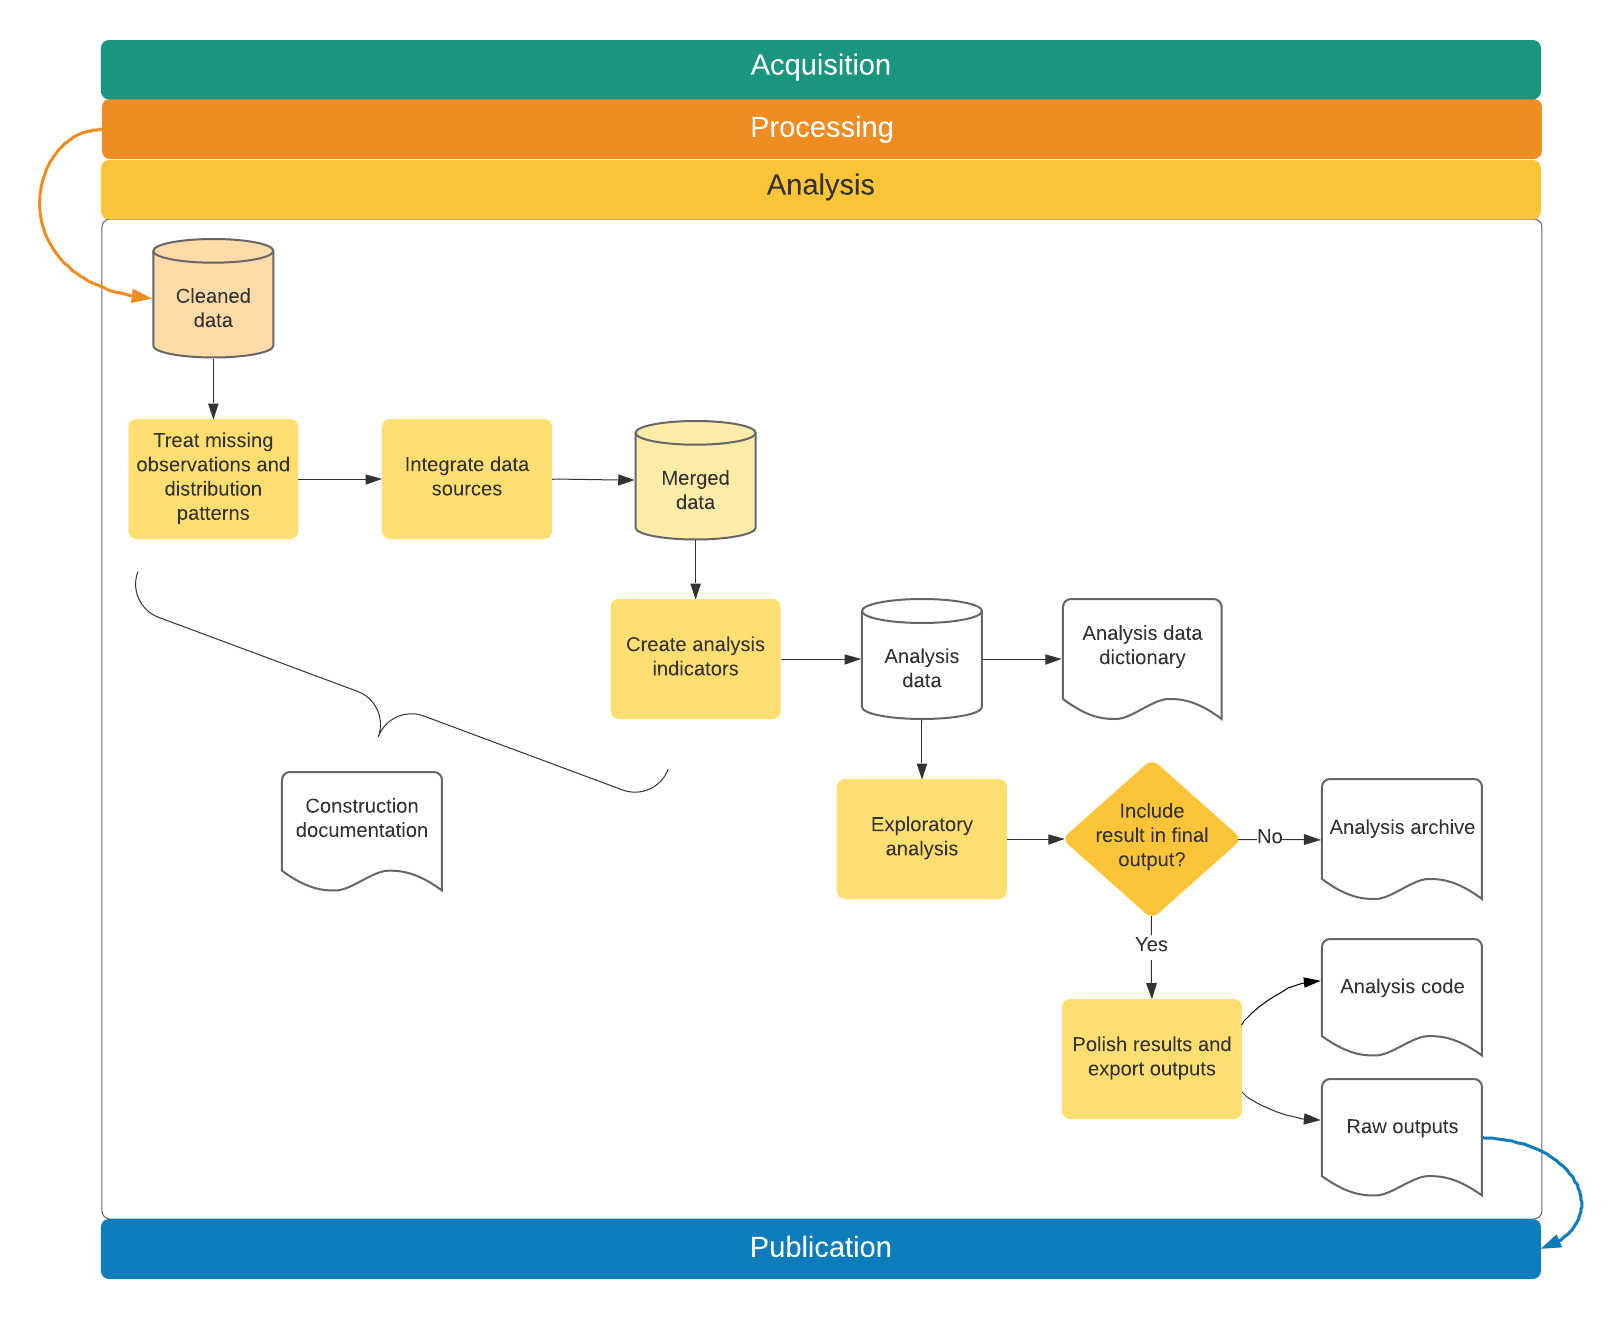
\includegraphics[width=1.6\linewidth]{diagrams/Analysis}
		\label{fig:analysis}
	\end{figure}
\end{fullwidth}

%------------------------------------------------


%----------------------------------------------------------------------------------------
%	CHAPTER 7
%----------------------------------------------------------------------------------------

\chapter{Chapter 7: Publishing research outputs}
\label{ch:7}

%------------------------------------------------

\begin{fullwidth}
Publication typically involves multiple iterations of manuscript,
code, and data files, with inputs from multiple collaborators.
This process can quickly become unwieldy.
It is in nobody's interest for a skilled and busy researcher
to spend days re-numbering references (and it can take days)
when a small amount of up-front effort can automate the task.
Similarly, simultaneous collaboration should not involve
the repetitive and error-prone task of manually resolving
sets of tracked-changes documents with conflicting edits.
Futhermore, for most research projects,
completing a manuscript is not the end of the task.
Academic journals often require a ``reproducibility package''
which contains the code and materials used to create the results.
These represent an intellectual contribution in their own right,
because they enable others to learn from your process
and better understand the results you have obtained.
Holding code and data to the same standards as written work
is a new practice for many researchers.

In this chapter, we suggest tools and workflows for efficiently managing collaboration
and ensuring reproducibility.
First, we discuss how to use dynamic documents to collaborate on technical writing.
Second, we provide guidelines for preparing a functioning and informative reproducibility package.
If you have organized your analytical process
according to the general principles outlined in earlier chapters,
preparing to publish materials will not require
substantial reorganization of the work you have already done.
Hence, publication is the conclusion of the system
of transparent, reproducible, and credible research we introduced
from the very first chapter of this book.
We include specific guidance on publishing both code and data files,
noting that these can be a significant contribution in addition to written results.
In all cases, we note that technology is rapidly evolving
and that specific tools noted here may not remain cutting-edge,
but the core principles involved in publication and transparency will endure.
\end{fullwidth}

%------------------------------------------------

\section{Preparing written documents for publication}

% collaborating is easier with dynamic documents
Development research is increasingly a collaborative effort.
This reflects changes in the economics discipline overall:
the number of sole-authored papers is decreasing,
and the majority of recent papers in top journals have three or more
authors.\sidenote{\url{https://voxeu.org/article/growth-multi-authored-journal-articles-economics}}
As a consequence, manuscripts typically pass back and forth between several writers
before they are ready for publication.
Just as with the preparation of analytical outputs,
effective collaboration requires the adoption of tools and practices
that enable version control and simultaneous contribution.
As we outlined in the previous chapter,
\textbf{dynamic documents} are a way to simplify writing workflows:
updates to analytical outputs that appear in these documents, such as tables and figures,
can be passed in to the final output with a single process,
rather than copy-and-pasted or otherwise handled individually.
Managing the writing process in this way
improves organization and reduces error,
such that there is no risk of materials being compiled
with out-of-date results, or of completed work being lost or redundant.

\subsection{Preparing manuscripts as {\LaTeX} documents}

% what exactly is a dynamic document
The most widely used software
for dynamically managing academic manuscripts is {\LaTeX} (pronounced ``lah-tek'').
\index{\LaTeX}
{\LaTeX} is a document preparation and typesetting system with a unique syntax.
While this tool has a significant learning curve,
its enormous flexibility in terms of operation, collaboration, output formatting, and styling
make it the primary choice for most large technical outputs.
It enables a streamlined collaboration workflow
that allows explicitly encoded references to raw output files.
This means that, whenever raw outputs are updated and the document is compiled,
it will automatically include the latest versions of all outputs.
This is not possible by default in Microsoft Word,
although there are add-ons that produce similar functionality.
In Word, you have to copy and paste each object
whenever tables, graphs, or other inputs are updated.
This creates complex inefficiency: updates may be accidentally excluded,
and ensuring they are not becomes more difficult as the document grows.
As time goes on, it becomes more and more likely
that a mistake will be made or something will be missed.
This is a broadly unsuitable way to prepare technical documents.

% advantages of LaTeX
In {\LaTeX}, instead of writing in a
``what-you-see-is-what-you-get'' mode as you do in Word,
you write plain text in a \texttt{.tex} file,
interlaced with coded instructions for formatting (similar to HTML).
{\LaTeX} enables automatically-organized documents,
manages tables and figures dynamically,
and includes commands for simple markup
like font styles, paragraph formatting, section headers and the like.
It includes special controls for including tables and figures,
footnotes and endnotes, complex mathematical notation, and automated bibliography preparation.
It also allows publishers to apply global styles and templates to already-written material,
allowing them to reformat entire documents in house styles with only a few keystrokes.

% keeping it simple
To create a {\LaTeX} manuscript,
you will typically create a new top-level directory for each final output.
Many projects go so far as to create documents like the main text
and any appendix text as separate projects.
For a single output, one convention is to put the manuscript files
(such as \texttt{main.tex} and \texttt{bibliography.bib})
in the top-level folder,
and then have the folders for figures, tables, and other inputs.
Your analytical scripts should easily be able to produce outputs
at the location of your choice by adjusting paths in the master script;
output them here when ready.
Above all, keep your workflow as simple as possible.
While {\LaTeX} \texit{can} produce complex formatting,
this is rarely needed for academic publishing,
as your manuscript will usually be reformatted in publication any
based on the style of the publisher.
Stick to the very basic {\LaTeX} tools:
the title page, manuscript sections and subsections,
figures and tables, mathematical equations,
bolding and italics, footnotes and endnotes,
and, last but not least, references and citations.

% managing references in LaTeX
One of the most important tools available in {\LaTeX}
is the BibTeX citation and bibliography manager.\cite{kopka1995guide}
BibTeX keeps all the references you might use in an auxiliary \texttt{.bib} file,
then references them using a simple command typed directly in the document.
Specifically, {\LaTeX} inserts references in text using the \texttt{\textbackslash cite\{\}} command.
Once this is written, {\LaTeX} automatically pulls all the citations into text
and creates a complete bibliography based on the citations you used whenever you compile the document.
The system allows you to specify exactly how references should be displayed in text
(such as superscripts, inline references, etc.)
as well as how the bibliography should be styled and in what order
(such as Chicago, MLA, Harvard, or other common styles).
The same principles that apply to figures and tables are therefore applied here:
You can make changes to the references in one place (the \texttt{.bib} file),
and then everywhere they are used they are updated correctly with one process.
BibTeX is so widely used that it is natively integrated in Google Scholar.
To obtain a reference in the \texttt{.bib} format for any paper you find,
click ``BibTeX'' at the bottom of the Cite window (below the preformatted options).
Then, copy the code directly into your \texttt{.bib} file.
They will look like the following:

\codeexample{sample.bib}{./code/sample.bib}

\noindent BibTeX citations are then used as follows:

\codeexample{citation.tex}{./code/citation.tex}

With this tool, you can ensure that references are handled
in a format you can manage and control.\cite{flom2005latex}
By changing some settings in the document itself,
you can change the style of inline citations and bibliographical references.
You can, for example, use superscripts or author names inline,
and order the bibiliography either by order of appearance or alphabetically.
All the formatting and numbering will be handled automatically.
You can also choose to display only the references which are cited in the text,
or to include every reference in the \texttt{.bib} file.
Since different publications have different requirements,
the ability to adapt this and other formatting very quickly,
including through using publisher-supplied templates where available.

% using pandoc to convert LaTeX into word
{\LaTeX} has one more useful trick:
using \textbf{\texttt{pandoc}},\sidenote{
  \url{https://pandoc.org}}
you can translate the raw document into Word
(or a number of other formats)
by running the following code from the command line:

\codeexample{pandoc.sh}{./code/pandoc.sh}

\noindent Conversion to Word is still required for a number of publishers.
You still don't want to write in Word, though.
The \texttt{pandoc} utility can only handle relatively simple formatting,
but it will seamlessly translate all the features we mentioned before
into the correct native Word styling.
The bracketed portion after \texttt{csl=} specifies the bibliography style;
this must be set manually for this conversion to work.
You can download a CSL (Citation Styles Library) file\sidenote{
  \url{https://github.com/citation-style-language/styles}}
for nearly any journal and have it applied automatically in this process.
Therefore, even in the case where you are required to provide
\texttt{.docx} versions of materials to others, or tracked-changes versions,
you can create them effortlessly from a {\LaTeX} manuscript,
then use external tools like Word's compare feature
to generate outputs like integrated track-changes versions when needed.


\subsection{Getting started with {\LaTeX} as a team}

{\LaTeX} is a challenging tool to get started using,
but the control it offers over the writing process is invaluable.
Because it is written in a plain text file format,
\texttt{.tex} can be version-controlled using Git.
This makes it possible to set up a dedicated GitHub repository for each output
and manage contributions and version histories
using the same system we recommend for analytical work.
DIME Analytics has created a variety of templates and resources
that you can adapt for your own team.\sidenote{
	\url{https://github.com/worldbank/DIME-LaTeX-Templates}}
Integrated editing and compiling tools like TeXStudio\sidenote{
  \url{https://www.texstudio.org}}
and \texttt{atom-latex}\sidenote{
  \url{https://atom.io/packages/atom-latex}}
offer the most flexibility to work with {\LaTeX} in teams.

% cloud-based implementations are a good place to start
Unfortunately, despite these advantages, {\LaTeX} can be a challenge to set up and us,
particularly if you are new to working with plain text code and file management.
It is also unfortunately weak with spelling and grammar checking.
This is because {\LaTeX} requires that all formatting be done in its special code language,
and it is not particularly informative when you do something wrong.
This can be off-putting very quickly for people
who simply want to get to writing, like senior researchers.
They can require a lot of troubleshooting at a basic level at first,
and staff not used to programming may not easily acquire the necessary knowledge.

In order to make it as easy as possible for your team
to use {\LaTeX} without all members having to invest in new skills,
we suggest using a cloud-based implementation as your first foray into {\LaTeX} writing.
Some teams even adopt these tools as a permanent solution.
Most such sites offer a subscription feature
with useful extensions and various sharing permissions,
and some offer free-to-use versions with basic tools that are sufficient
for a broad variety of applications,
up to and including writing a complete academic paper with coauthors.

% Advantages of cloud-based implementations
Cloud-based implementations of {\LaTeX} have several advantageous features
for teams compared to classic desktop installations.
First, since they are completely hosted online,
they avoid the inevitable troubleshooting required to set up a {\LaTeX} installation
on various personal computers run by the different members of a team.
Second, they typically maintain a single, continuously synced, master copy of the document
so that different writers do not create conflicted or out-of-sync copies,
or need to deal with Git themselves to maintain that sync.
Third, they typically allow collaborators to edit documents simultaneously,
though different services vary the number of collaborators and documents allowed at each tier.
Fourth, and most usefully, some implementations provide a ``rich text'' editor
that behaves pretty similarly to familiar tools like Word,
so that collaborators can write text directly into the document without worrying too much
about the underlying {\LaTeX} coding.
Cloud services also usually offer a convenient selection of templates
so it is easy to start up a project and see results right away
without needing to know a lot of the code that controls document formatting.

% Disadvantages of cloud-based implementations
Cloud-based implementations of {\LaTeX} also have disadvantages.
There is still some up-front learning required, unless you're using the rich text editor.
Continuous access to the Internet is necessary,
and updating figures and tables requires a bulk file upload that is tough to automate.
They vary dramatically in their ability to integrate
with file systems where you store your code and outputs,
and so you will need to practice an integrated workflow depending what is available to you.
Despite this, we believe that with minimal learning and workflow adjustments,
cloud-based implementations are often the easiest way to allow coauthors to write and edit in \LaTeX,
so long as you make sure you are available to troubleshoot minor issues like these.

%----------------------------------------------------

\section{Preparing and publishing data}

% what are reproducibility packages and what they must contain
While we have focused so far on written materials,
it is also important to consider how you will publish
the data you used for your research.
The open science community at large sees data publication
both as a citable output and as a necessary transparency measure.
Fortunately, it is a conceptually simple task for you to produce
and archive or catalog the required materials.
Beginning from the raw data that you collected,
you should be prepared to catalog two separate collections.
First, you should catalog the unaltered (de-identified) data
with all variables corresponding directly
to fields in the original dataset or data collection instrument.
Second, you should separately catalog (as supporting material)
the analytical dataset used for the output you are publishing.
This release should include the data construction scripts
that create transformed and derived indicators,
as well as project-specific information
such as treatment assignment and other indicators
that were not directly acquired during fieldwork.

\subsection{De-identifying data for publication}

% what is final de identification
Before publishing data,
you should carefully perform a \textbf{final de-identification}.
Its objective is to reduce the risk of disclosing confidential information in the published dataset.
If you are following the steps outlined in this book,
you should have already removed direct identifiers after collecting the data.
Direct identifiers are data elements that are keyed to the identity of a respondent,
such as names, phone numbers, official identification numbers like government IDs.
Direct identifiers further include all information that may easily be linked to public records,
such as dates of birth, job titles, marital records, and other personal vital statistics.

At this stage, however, you should additionally remove
indirect identifiers, and assess the statistical disclosure risk of your data.\sidenote{
	\textbf{Disclosure risk:} the likelihood that a released data record can be associated with an individual or organization.}\index{statistical disclosure}
Unlike direct identifiers, for which a link (or lack thereof) to public information is verifiable,
indirect identifiers require an assessment of both the likelihood
that an individual can be singled out in the data
and then linked to public information in complex combinations.
For example, with sufficiently small population groups like US ZIP codes,
the age and gender of a respondent may be enough to identify them.
This will also often be the case in development work,
where information such as the size of a household,
the ages and marital statuses of the household members,
and the types of work or schooling they engage in
may be more than enough to identify a person or family
from a sufficiently small group.

It also requires an assessment of the potential risk to the individual
that could be caused by disclosure of their identity or personal information.
This will vary widely depending on the types of information
you are collecting and the overall vulnerability of the population.
In extreme cases, where the population is highly vulnerable
and combinations of information are highly specific,
you may not be able to publicly release any data at all.
You will still be expected to catalog and cite your data,
even if you will not be expected to archive it outside your approved internal system.
To the extent required to ensure reasonable privacy,
potentially identifying variables must be further masked or removed.

% tools for final de-identification: pii_detection, pii-scan, sdcMicro
There are a number of tools developed to help researchers de-identify data
and which you should use as appropriate at that stage of data collection.
These include \texttt{PII\_detection}\sidenote{
	\url{https://github.com/PovertyAction/PII\_detection}}
from IPA,
\texttt{PII-scan}\sidenote{
	\url{https://github.com/J-PAL/PII-Scan}}
from JPAL,
and \texttt{sdcMicro}\sidenote{
	\url{https://sdcpractice.readthedocs.io/en/latest/sdcMicro.html}}
from the World Bank.
\index{anonymization}
The \texttt{sdcMicro} tool, in particular, has a feature
that allows you to assess the uniqueness of the records in your data.
It produces simple measures of the identifiability of records from
the combination of potentially indirectly identifying variables,
and allows you to apply common information masking algorithms,
such as binning, top-coding, and jittering data prior to release.
You should determine how sensitive your results are to these transformations
if you need to release data from which your exact results
cannot be reproduced for this reason.

% trade-off between accuracy and privacy
There will almost always be a trade-off between accuracy and privacy.
For publicly disclosed data, you should favor privacy.
Stripping identifying variables from a dataset may not be sufficient to protect respondent privacy,
due to the risk of re-identification.
One potential solution is to add noise to data, as the US Census Bureau has proposed.\cite{abowd2018us}
This makes the trade-off between data accuracy and privacy explicit.
But there are not, as of yet, established norms for such ``differential privacy'' approaches:
most approaches fundamentally rely on judging ``how harmful'' information disclosure would be.
The fact remains that there is always a balance between information release (and therefore transparency)
and privacy protection, and that you should engage with it actively and explicitly.
The best thing you can do is make a complete record of the steps that have been taken
so that the process can be reviewed, revised, and updated as necessary.

% restricting access of confidential for reproducibility check
In cases where confidential data is required for analysis,
we recommend embargoing sensitive or access-restricted variables when publishing the dataset.
In practice, if you have a secure repository from your
home institution, funding institution, or other collaborator,
you can store the data there
and publish only a catalog entry
indicating that the data is not available for general publication.
Access to the embargoed data could be granted for specific purposes,
such as a computational reproducibility check required for publication,
if done under careful data security protocols and approved by an IRB.

\subsection{Publishing raw and constructed datasets}

% options for when the data cannot be published
Publicly documenting all original data generated as part of a research project
is an important contribution in its own right.
Cataloging and/or archiving original datasets
is a significant contribution that can be made
in addition to any publication of analysis results.\sidenote{
	\url{https://www.povertyactionlab.org/sites/default/files/resources/J-PAL-guide-to-publishing-research-data.pdf}}
If you are not able to publish the data itself,
due to licensing agreements or ethical concerns,
there are often options to catalog or archive the data.
These may take the form of metadata catalog entries or embargoed releases.
Such setups allow you to hold an archival version of your data
which your publication can reference,
and provide information about the contents of the datasets
and how future users might request permission to access them
(even if you are not the person to grant that permission).
They can also provide for timed future releases of datasets
once the need for exclusive access has ended.
In all cases, you should choose a method that allows you
to obtain a digital object identifier (DOI)
and a formal citation for your data to use in your publication.

% platforms for publishing data
Publicly releasing data allows other researchers
to validate the mechanical construction of your results,
investigate what other results might be obtained from the same population,
and test alternative approaches or answer other questions.
This fosters collaboration and may enable researchers to explore variables and
questions that you do not have time to focus on otherwise.
There are different options for public data release.
The World Bank's Development Data Hub\sidenote{
	\url{https://datacatalog.worldbank.org}}
includes a Microdata Catalog\sidenote{
\url{https://microdata.worldbank.org}}
and a Geospatial Catalog,
where researchers can publish data and documentation for their projects.\sidenote{
\url{https://dimewiki.worldbank.org/Microdata\_Catalog}
\newline
\url{https://dimewiki.worldbank.org/Checklist:\_Microdata\_Catalog\_submission}
}
The Harvard Dataverse\sidenote{
	\url{https://dataverse.harvard.edu}}
publishes both data and code.
The Datahub for Field Experiments in Economics and Public Policy\sidenote{\url{https://dataverse.harvard.edu/dataverse/DFEEP}}
is especially relevant for impact evaluations.
Both the World Bank Microdata Catalog and the Harvard Dataverse
create data citations for deposited entries.
DIME has its own collection of datasets in the Microdata Catalog,
where data from our projects is published.\sidenote{\url{
		https://microdata.worldbank.org/catalog/dime}}

% check what you can and cannot publish
Raw de-identified data can and should be published
as an independent entity with its own license.
It should be named according to the data collection effort
or the project that supported its collection,
rather than tied to a specific research output.
This makes it easy for you or others to access and cite that dataset.
However, even when your raw data is owned by someone else,
or for any other reason you are not able to publicly release it,
you will often still retain the rights to release derived and constructed data,
even if they contain only the indicators you created and their documentation.\sidenote{
  \url{https://guide-for-data-archivists.readthedocs.io}}
Regardless of what may be done with the raw data,
you will therefore typically be able to separately license or publish
the derived dataset and the indicators needed for analysis
as citable supporting materials for any publication.
Many of the resources above will support this type of release.
The OSF offers a useful functionality to self-publish materials of this form,
and some publishers (such as the AEA) offer in-house handling of these materials.
If you have questions about your rights over original or derived materials,
check with the legal team at your organization or with the data provider.
Make sure you understand the rights associated with any data release
and communicate them to any future users of the data.

% licensing published data
When you do publish data that you own,
you will decide how it may be used and what license,
if any, you will assign to it.\sidenote{
  \url{https://iatistandard.org/en/guidance/preparing-organisation/organisation-data-publication/how-to-license-your-data}}
In all cases, material without a license may never be reused;
you should prefer to offer a license that is explicit
and details whether and how specific individuals may access the data.
Terms of use available in the World Bank Microdata Catalog include,
in order of increasing restrictiveness:
open access, direct access, and licensed access.\sidenote{
  \url{https://microdata.worldbank.org/index.php/terms-of-use}}
Open Access data is freely available to anyone, and simply requires attribution.
Direct Access data is available to registered users who agree
to use the data for statistical and scientific research purposes only,
to cite the data appropriately,
and not to attempt to identify respondents or data providers
or link the data to other datasets that could allow for re-identification.
Licensed access data is restricted to bona fide users,
who submit a documented application detailing
how they will use the data and then sign a formal agreement governing data use.
The user must be acting on behalf of an organization,
which will be held responsible in the case of any misconduct.

% content of data publication: data files, meta data and dcumentation
Published data should be released in a widely recognized format.
While software-specific datasets are acceptable accompaniments to the code
(since those precise materials are probably necessary),
you should also consider releasing datasets in plain text formats
such as CSV files with accompanying codebooks,
since these can be used by any researcher.
Additionally, you should also release PDF or code versions of
the data collection instrument or survey questionnaire
so that readers can understand which data components are
collected directly in the field and which are derived.
With your analytical dataset,
you should also release the code
that constructs any derived measures
from the raw dataset,
so that others can learn from your work and adapt it as they like.

\section{Preparing a complete reproducibility package}

Major journals now often require that,
in addition to the data required to obtain your results,
you provide the code that exactly recreates those results.
Some even require being able to reproduce the results themselves
before they will approve a paper for publication.\sidenote{
  \url{https://www.aeaweb.org/journals/policies/data-code}}
This set of materials, taken together,
is often referred to as a ``reproducibility package''.
If your material has been well-structured throughout the analytical process,
this will only require a small amount of extra work;
if not, creating this package may take some time.
When it is completed,
whoever downloads it should be able
to understand how your code produces results from your data
and be able to reproduce them by executing the included master script.

\subsection{Organizing code for reproducibility}

% published code must be understandable
Before releasing your code, you should edit it for content and clarity
just as if it were written material.
The purpose of releasing code is to allow others to understand
exactly what you have done in order to obtain your results,
as well as to apply similar methods in future projects.
They should also be able to make small adjustments to your code
and reproduce individual portions of your analysis
so they can understand the choices and functions you implemented.
The code should both be functional and readable,
through the use of clean structure and extensive commenting and documentation.
Code is often not written this way when it is first prepared,
so it is important for you to review the content and organization
so that a new reader can figure out what and how your code should do.
Whereas your data should already be relatively clean by this stage,
your code is much less likely to be so.
This is often where you need to invest time prior to releasing your reproducibility package.

% reproducibility review
DIME has adopted several practices and requirements to support the production
of high-quality reproducibility packages by its researchers.
The materials for these practices are publicly available,
so you can use them to check the reproducibility of your own work.
DIME code must be submitted for a computational reproducibility check
before publication as a working paper or submission to a journal.
This reproducibility check is initiated by contacting the DIME Analytics team
and submitting the Reproducibility Package Checklist.
In addition to this formal requirement for reproducibility review,
DIME projects are required to be maintained continuously at high quality.
These practices must include ensuring that project code is organized
with a master script so that computational reproducibility is a one-click exercise.
DIME projects are also expected to use Git and GitHub
to document project work and collaboration,
and to keep the master branch up-to-date as a working edition.
Research assistants also participate in quarterly peer code review rounds
so that they can improve their code and documentation as it is written,
and not be required to revisit it in a rush near publication time.

% ensuring code reproducibility
Before releasing the code, make sure it functions identically on a fresh install of your chosen software.
A new user should have no problem getting the code to execute perfectly.
In either a scripts folder or in the root directory,
you should include a master script that allows the reviewer to run the entire project
and re-create all raw outputsby changing only a single line of code:
the one setting the directory path.
To ensure that your code will run completely on a new computer,
you must install any required user-written commands in the master script
(for example, in Stata using \texttt{ssc install} or \texttt{net install}
and in R include code giving users the option to install packages,
including selecting a specific version of the package if necessary).
In many cases you can even directly provide the underlying code
for any user-installed packages that are needed to ensure forward-compatibility.
Make sure system settings like \texttt{version}, \texttt{matsize}, and \texttt{varabbrev} are set.

% tracking code and outputs
Finally, make sure that code inputs and outputs are clearly identified.
A new user should, for example, be able to easily find and remove
any files created by the code so that they can be recreated quickly.
They should also be able to quickly map all the outputs of the code
to the locations where they are placed in the associated published material,
so ensure that the raw components of figures or tables are clearly identified.
Documentation in the master script is often used to indicate this information.
For example, outputs should clearly correspond by name to an exhibit in the paper, and vice versa.
(Supplying a compiling {\LaTeX} document can support this.)
Code and outputs which are not used should be removed before publication.

\subsection{Releasing a reproducibility package}

% finding a place to publish the package
Once your data and code are polished for public release,
all you need to do is find a place to publish your materials.
This is slightly easier said than done,
as there are a few variables to take into consideration
and, at the time of writing, no global consensus on the best solution
and there are a variety of archives and storage providers
that cater to different needs.
The technologies available are likely to change dramatically
over the next few years;
the specific solutions we mention here highlight some current approaches
as well as their strengths and weaknesses.

% code licenses
Unlike data, code usually has few external constraints to publication.
The research team owns the code in almost all cases,
and code is unlikely to contain identifying information
(though you must check carefully that it does not).
Publishing code also requires assigning a license to it;
in a majority of cases, code publishers like GitHub
offer extremely permissive licensing options by default.
If you do not provide a license, nobody can use your code.
You may be required to put your materials into the public domain;
if not, it is common to only require attribution and citation for their reuse,
without putting any barriers or restrictions to accessing the code.

% pros and cons of GitHub
One option for releasing a reproducibility package is GitHub.
Making a public GitHub repository is completely free.
It can hold any file types,
provide a structured, compressed download of your whole project,
and allow others to look at alternate versions or histories easily.
It is straightforward to simply upload a fixed directory to GitHub,
apply a sharing license, and obtain a URL for the whole package.
There is a strict size restriction of 100MB per file and
a restriction of 100GB on the size of the repository as a whole,
so larger projects will need alternative solutions.
However, GitHub is not the ideal platform to release reproducibility packages.
It is built to version control code, and to facilitate collaboration on it.
It is not an archive, meaning that it does not guarantee the permanence
of uploaded materials, it does not guarantee the permanence of the access URL,
and it does not manage citations or non-code licenses by default.

Features to look for in a platform to release reproducibility packages include:
the possibility to store data and documentation as well as code,
the creation of a static copy of its content, that cannot be changed or removed,
and the assignment of a permanent digital object identifier (DOI) link.
One suggestion is to combine GitHub with the Open Science Framework,\sidenote{
  \url{https://osf.io}}
as OSF can easily link to and import material from GitHub and
apply a permanent URL, DOI, formal citation, general license, and archival services to it.

% Other options: data verse, osf, research gate. what to look for before deciding
Other options include the Harvard Dataverse\sidenote{
  \url{https://dataverse.harvard.edu}}
and ResearchGate.\sidenote{
  \url{https://https://www.researchgate.net}}
Any of these archival services is acceptable --
the main requirement is that the system can handle
the structured directory that you are submitting,
and that it can provide a stable, structured URL for your project
and report exactly what, if any,
modifications you have made since initial publication.
You can even combine more than one tool if you prefer,
as long as they clearly reference each other.
For example, one could publish code and the corresponding license on GitHub
and point to data published on the World Bank Microdata Catalog.
Emerging technologies such as the ``containerization'' approach of CodeOcean\sidenote{
  \url{https://codeocean.com}}
offer to store both code and data in one repository,
and also provide an online workspace in which others can execute and modify your code
without having to download your tools and match your local environment
when packages and other underlying software may have changed since publication.
In a similar spirit, attempts to create ``metadata archives''
that link all the different materials, releases, and publications
relating to specific research projects or studies
offer an avenue for improving the organization of these materials in the future.

% pre-prints
In addition to code and data,
you may also want to release an author's copy or preprint
of the article itself along with these raw materials.
Check with your publisher before doing so;
not all journals will accept material that has been publicly released
before its formal publication date, although,
in most development research fields,
the release of working papers is a fairly common practice.
This can be done on a number of preprint websites,
many of which are topic-specific.\sidenote{
  \url{https://arxiv.org/}}
You can also use GitHub or OSF and link to the PDF file directly
through your personal website or whatever medium you are sharing the preprint.
However, do not use Dropbox or Google Drive for this purpose:
many organizations do not allow access to these tools,
and staff may be blocked from accessing your material.


%----------------------------------------------------------------------------------------
%	Conclusion
%----------------------------------------------------------------------------------------

\chapter*{Bringing it all together} % The asterisk leaves out this chapter from the table of contents

We hope you have enjoyed \textit{Development Research in Practice: The DIME Analytics Data Handbook}.
Our aim was to teach you to handle data more efficiently, effectively, and ethically.
We laid out a complete vision of the tasks of a modern researcher,
from planning a project's data governance to publishing code and data
to accompany a research product.
We have tried to set the text up as a resource guide
so that you will always be able to return to it
as your work requires you to become progressively more familiar
with each of the topics included in the guide.

We started the book with a discussion of 
credibility, transparency, and reproducibility in research:
an overarching idea that your work should always be
accessible and available to others, both within and outside your team.
We then discussed the current research work environment,
which necessitates cooperation with a diverse group of collaborators
using modern approaches to computing technology.
We outlined methods for planning your data work
and creating basic documentation for data,
so that multiple data sources can be linked without error
and so that you can map the structure of your data
to your research design.
We discussed how to implement reproducible routines for sampling and randomization,
and to analyze statistical power and use randomization inference.

We detailed modern data acquisition methods and frameworks,
including data licensing, data ownership,
electronic data collection, and data security.
We provided a detailed workflow for data cleaning and processing,
emphasizing tidy data, quality control, privacy protection, and documentation.
We discuss the creation of derived indicators and analysis outputs,
and give an overview of the workflow required to move these results
to publication -- no matter the format of your work --
as well as tools and practices for making this work publicly accessible.
Throughout, we emphasized that data work is a ``social process'',
involving multiple team members with different roles and technical abilities.
This mindset and workflow, from top to bottom,
outline the tasks and responsibilities
that are fundamental to doing credible research.

However, as you probably noticed, the text itself provides
just enough detail to get you started:
an understanding of the purpose and function of each of the core research steps.
The references and resources get into the details
of how you will realistically implement these tasks:
from DIME Wiki pages detail specific code conventions
and field procedures that our team considers best practices,
to the theoretical papers that will help you figure out
how to handle the unique cases you will undoubtedly encounter.
We hope you will keep the book on your desk
(or the PDF on your desktop)
and come back to it anytime you need more information.
We wish you all the best in your work
and will love to hear any input you have on ours!\sidenote{
You can share your comments and suggestion on this book through \url{https://worldbank.github.io/dime-data-handbook}.}

\vspace{1cm}
\begin{fullwidth}
	\begin{figure}
		\centering
		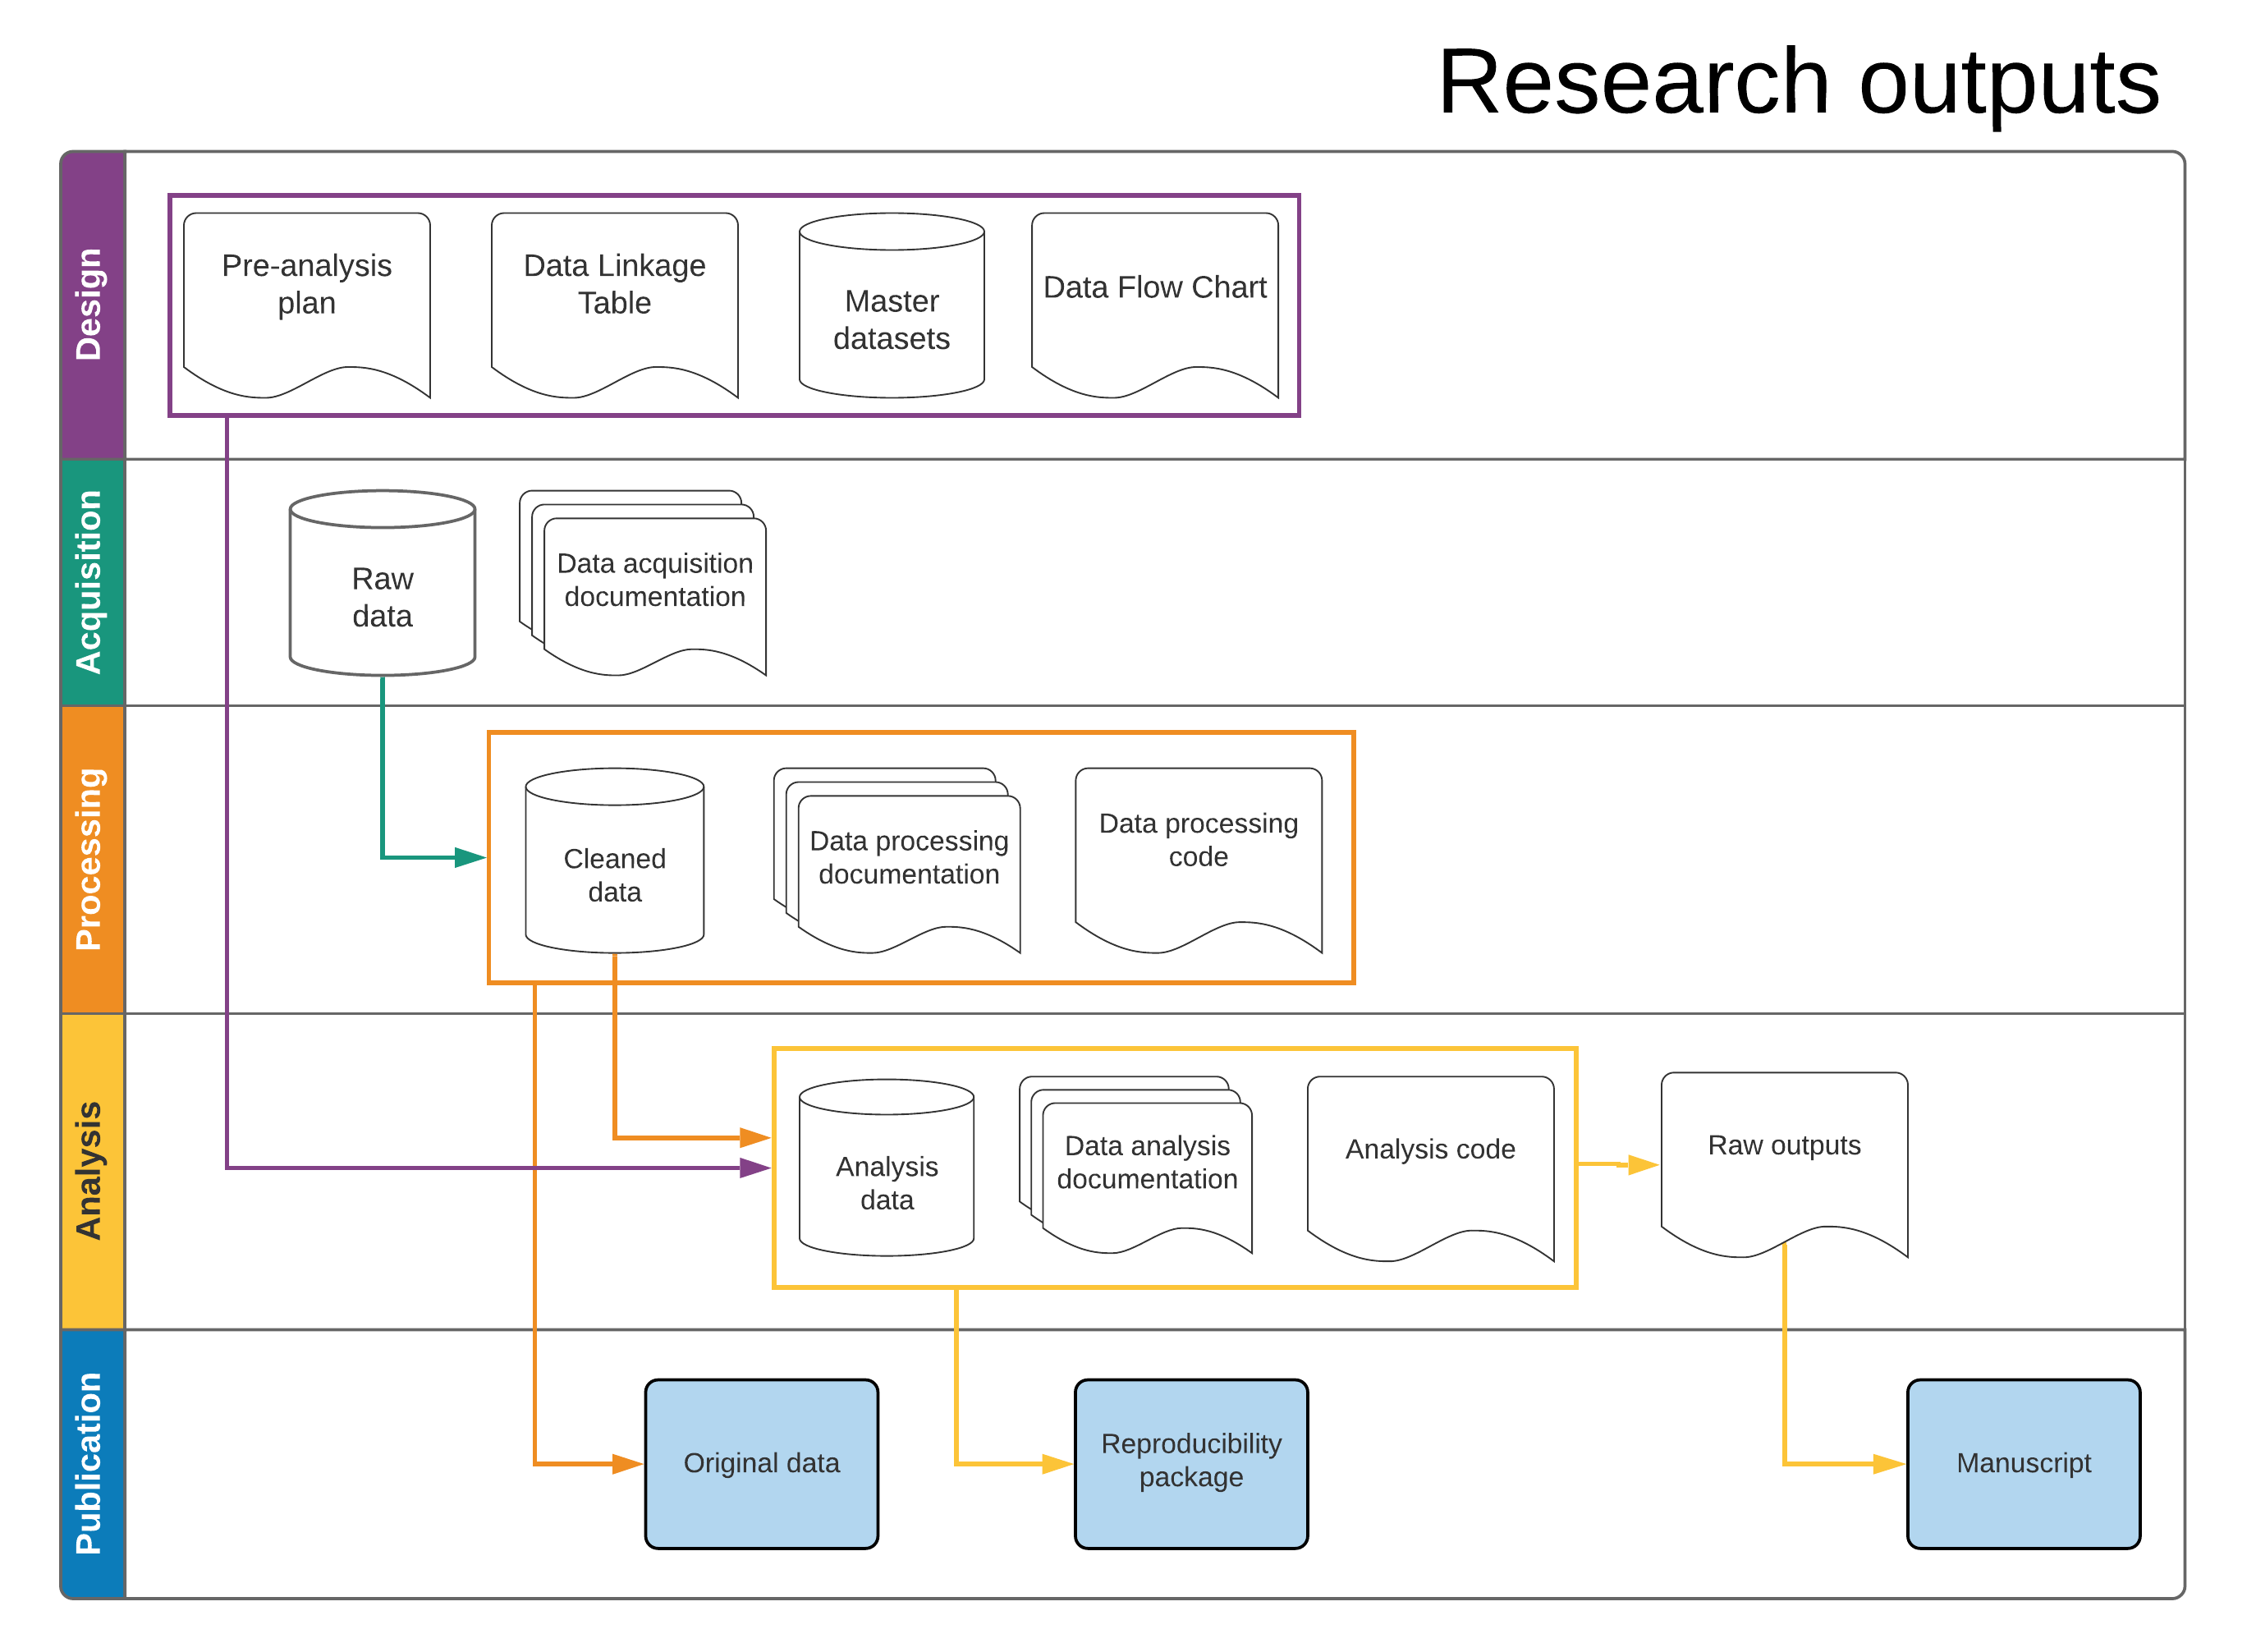
\includegraphics[width=1.6\linewidth]{diagrams/Conclusion}
		\caption{}
		\label{fig:intro}
	\end{figure}
\end{fullwidth}


%----------------------------------------------------------------------------------------
%	APPENDIX : Stata Style Guide
%----------------------------------------------------------------------------------------

\chapter{Appendix: The DIME Analytics Stata Style Guide}
\label{ap:1}

%------------------------------------------------

\begin{fullwidth}

Most academic programs that prepare students for a career
in the type of work discussed in this book
spend a disproportionately small amount of time
teaching their students coding skills
in relation to the share of their professional time
they will spend writing code
in their first few years after they graduate.
Recent masters-level graduates joining our team
have shown very good theoretical knowledge
while requiring a lot of training in practical skills.
To us, this is like an architecture graduate having learned
how to sketch, describe, and discuss
the concepts and requirements of a new building very well --
but without the technical ability
to contribute to a blueprint following professional standards
that can be used and understood by others.
The reasons for this are a topic for another book,
but in today's data-driven world,
people working in quantitative development research
must be proficient collaborative programmers,
and that includes more than being able to compute correct numbers.

This appendix begins with a section on some general and language-agnostic
principles on how to write ``good'' code.
Good code is code that both generates correct results \textit{and}
is easily read and adapted by other professionals.
The second section in this appendix contains instructions
on how to access and use the code examples in this book.
The last section contains the DIME Analytics Stata Style Guide.
Widely accepted and used style guides are common in most programming languages,
but we have never found a sufficiently encompassing style guide for Stata.
We created this style guide having in mind practices that,
in our experience, greatly improve the quality
of research projects coded in Stata.
We hope that this guide can help increase the emphasis
given to using, improving, sharing, and standardizing code style
among the Stata community.
We believe these resources can help anyone write more understandable code,
and how you, like an architect,
can create a blueprint that can be understood and used
by everyone in your trade.

\end{fullwidth}

%------------------------------------------------

\section{Writing good code}

``Good'' code has two elements:
(1) it is correct, in that it doesn't produce any errors
and its outputs are the objects intended,
and (2) it is useful and comprehensible
to someone who hasn't seen it before
(or even someone who has, weeks, months, or years later).
Many researchers have only been trained to code correctly.
But we believe that when your code runs on your computer
and you get the desired results,
you are only half-done writing \textit{good} code.
Good code is easy to read and replicate,
making it easier to spot mistakes.
Good code reduces sampling, randomization, and cleaning errors.
Good code can easily be reviewed by others
before it's published and can be re-used afterwards.
We always tell people to ``code as if a stranger is reading it''.

You should think of good code in terms of three major elements:
\textbf{structure}, \textbf{syntax}, and \textbf{style}.
The \textbf{structure} is the environment
and file organization your code lives in:
good structure means that it is easy to find individual pieces of code,
within and across files,
that correspond to specific tasks and outputs.
It also means that functional code blocks
are sufficiently independent from each other
such that they can be shuffled around, repurposed,
and even deleted without affecting the execution of other portions.
The \textbf{syntax} is the literal language of your code.
Good syntax means that your code is readable
in terms of how its mechanics implement ideas --
it should not require arcane reverse-engineering
to figure out what a code chunk is trying to do.
It should use common commands in a generally accepted way
so others can easily follow and reconstruct your intentions.
Finally, \textbf{style} is the way
that the non-functional elements of your code convey its purpose.
Elements like spacing, indentation,
and naming conventions (or lack thereof)
can make your code much more
(or much less) accessible to someone
who is reading it for the first time
and needs to understand it quickly and accurately.

One key tool for writing good code is using help documentation.
Whether or not you are new to the programming language you are using
-- Stata, R, Python, or one of the many others --
you should constantly revisit help files for the most common commands.
Often you will learn they can do something you never realized.
We cannot emphasize enough how important it is
that you get into the habit of reading help files,
especially for commands you are very familiar with.
Most of us have a help file window open at all times.
Similarly, you will always run into commands or uses of commands that
you have not seen before or whose functionality you do not remember.
Every time that happens,
you should look up the help file for that command.
We often encounter the conception that help files are only for beginners.
We could not disagree with that conception more.
The only way to get better at the programming language you use
is to constantly read help files.

\section{Using the code examples in this book}

Providing some standardization for Stata code style
is also a goal of our team.
Stata is one of several programming languages used at DIME,
but since few high-quality resources based on Stata exist
relative to its importance and frequency of use,
we decided to use Stata for the examples in this book.
This book includes several code blocks
where we demonstrate a good code execution
of some of the most common tasks in data work.
We have ensured that each code block runs independently,
is well-formatted,
and uses built-in commands as much as possible.
We hope that these snippets will provide a foundation for your code style.
We try to comment code examples generously (as you should),
and you should reference Stata help files by writing \texttt{help [command]}
whenever you do not understand the command that is being used.
For example, if you are not familiar with \texttt{isid},
 then write \texttt{help isid},
and the help file for the command \texttt{isid} will open.
You should do this even if you know \texttt{isid}
but has not read the help file for that command in a while,
as there is always something new to learn.

In the book, code examples are presented like the following:

\codeexample{code.do}{./code/code.do}

You can access the raw code used in examples in this book in several ways.
We use GitHub to version control all the content of this book,
including the code examples.
To see the code examples on GitHub, go to:
\url{https://github.com/worldbank/dime-data-handbook/tree/master/code}.
We only use Stata's built-in datasets in our code examples,
so you do not need to download any data.
If you have Stata installed on your computer,
then you will already have the data files used in the code.

A less technical way to access the code
is to click the individual file in the URL above, then click
the button that says \textbf{Raw}.
You will then get to a page that looks like the one at:
\url{https://raw.githubusercontent.com/worldbank/dime-data-handbook/master/code/code.do}.
There, you can copy the code
from your browser window to your do-file editor with the formatting intact.
This method is only practical for a single file at a time.
If you want to download all code used in this book, you can do that at:
\url{https://github.com/worldbank/dime-data-handbook/archive/master.zip}.
That link downloads a \texttt{.zip} file
with all the content used in writing this book,
including the \LaTeX{} code used for the book itself.
After extracting the .zip-file you will find all the code in a folder called \texttt{/code/}.

While we use built-in commands as much as possible in this book,
we point to user-written commands when they provide important new functionality.
In particular, we point to two suites of Stata commands developed by DIME Analytics,
\texttt{ietoolkit}\sidenote{\url{https://dimewiki.worldbank.org/ietoolkit}} and
\texttt{iefieldkit},\sidenote{\url{https://dimewiki.worldbank.org/iefieldkit}}
which DIME Analytics wrote to standardize
core data collection, management, and analysis workflows.

When you encounter code that employs user-written commands,
you will not be able to run them or read their help files
until you have installed the commands.
The most common place to distribute user-written commands for Stata
is the Boston College Statistical Software Components (SSC) archive.\sidenote{
	\url{https://ideas.repec.org/s/boc/bocode.html}}
The user-written commands in our code example are all from the SSC archive.
So, if your installation of Stata does not recognize a command in our code, for example
\texttt{randtreat}, then type \texttt{ssc install randtreat} in Stata.

Some commands on SSC are distributed in packages.
This is the case, for example, of \texttt{ieboilstart}.
That means that you will not be able to install it using \texttt{ssc install ieboilstart}.
If you do, Stata will suggest that you instead use \texttt{findit ieboilstart},
which will search SSC (among other places) and see if there is a
package that contains a command called \texttt{ieboilstart}.
Stata will find \texttt{ieboilstart} in the package \texttt{ietoolkit},
so to use this command you will type \texttt{ssc install ietoolkit} in Stata instead.

We understand that it can be confusing to work with packages for first time,
but this is the best way to set up your Stata installation to benefit from other
people's work that has been made publicly available.
Once you get used to installing commands like this it will not be confusing at all.
All code with user-written commands, furthermore, is best written when it installs such commands
at the beginning of the master do-file,
so that the user does not have to search for packages manually.

\section{The DIME Analytics Stata Style Guide}

Programming languages used in computer science
always have style guides associated with them.
Sometimes they are official guides that are universally agreed upon,
such as PEP8 for Python.\sidenote{\url{https://www.python.org/dev/peps/pep-0008}}
More commonly, there are well-recognized but
non-official style guides like the JavaScript Standard Style\sidenote{\url{https://standardjs.com/\#the-rules}}
for JavaScript or Hadley Wickham's style guide for R.\sidenote{\url{https://style.tidyverse.org/syntax.html}}
Google, for example, maintains is own style guides for all languages
that are used in its projects.\sidenote{
  \url{https://github.com/google/styleguide}}

Aesthetics is an important part of style guides, but not the main point.
Neither is telling you which commands to use:
there are plenty of guides to Stata's extensive functionality.\sidenote{
  See for example \citet{Mark2012}}
The important function is to allow programmers who are likely to work together
to share conventions and understandings of what the code is doing.
Style guides therefore help improve the quality of the code
in that language that is produced by all programmers in a community.
It is through a shared style that newer programmers can learn from more experienced programmers
how certain coding practices are more or less error-prone.
Broadly-accepted style conventions make it easier to borrow solutions
from each other and from examples online
without causing bugs that might only be found too late.
Similarly, globally standardized style guides make it easier to solve each others'
problems and to collaborate or move from project to project,
and from team to team.

There is room for personal preference in style guides,
but style guides are first and foremost about quality and standardization --
especially when collaborating on code.
We believe that a commonly used Stata style guide
would improve the quality of all code written in Stata,
which is why we have begun the one included here.
You do not necessarily need to follow our style guide precisely.
We encourage you to write your own style guide if you disagree with us.
The best style guide would be the one adopted the most widely.
All style rules introduced in this section are the way we suggest to code,
but the most important thing is that the way you style your code is \textit{consistent}.
This guide allows our team to have a consistent code style.

\subsection{Commenting code}

Comments do not change the output of code, but without them,
your code will not be accessible to your colleagues.
It will also take you a much longer time to edit code you wrote in the past if you did not comment it well.
So, comment a lot: do not only write \textit{what} your code is doing
but also \textit{why} you wrote it like the way you did.
In general, try to write simpler code that needs less explanation,
even if you could use an elegant and complex method in less space,
unless the advanced method is a widely accepted one.

There are three types of comments in Stata and they have different purposes:

\codeexample{stata-comments.do}{./code/stata-comments.do}

\subsection{Abbreviating commands}

Stata commands can often be abbreviated in the code.
You can tell if a command can be abbreviated if the help file indicates an abbreviation by underlining part of the name in the syntax section at the top.
Only built-in commands can be abbreviated; user-written commands cannot.
(Many commands additionally allow abbreviations of options:
these are always acceptable at the shortest allowed abbreviation.)
Although Stata allows some commands to be abbreviated to one or two characters,
this can be confusing -- two-letter abbreviations can rarely be ``pronounced''
in an obvious way that connects them to the functionality of the full command.
Therefore, command abbreviations in code should not be shorter than three characters,
with the exception of \texttt{tw} for \texttt{twoway} and \texttt{di} for \texttt{display},
and abbreviations should only be used when widely a accepted abbreviation exists.
We do not abbreviate \texttt{local}, \texttt{global}, \texttt{save}, \texttt{merge}, \texttt{append}, or \texttt{sort}.
The following is a list of accepted abbreviations of common Stata commands:

\begin{center}
	\begin{tabular}{ c | l }
    Abbreviation & Command \\
		\hline
		\texttt{tw} & \texttt{twoway} \\
		\texttt{di} & \texttt{display} \\
		\texttt{gen} & \texttt{generate} \\
		\texttt{mat} & \texttt{matrix} \\
		\texttt{reg} & \texttt{regress} \\
		\texttt{lab} & \texttt{label} \\
		\texttt{sum} & \texttt{summarize} \\
		\texttt{tab} & \texttt{tabulate} \\
		\texttt{bys} & \texttt{bysort} \\
		\texttt{qui} & \texttt{quietly} \\
		\texttt{noi} & \texttt{noisily} \\
		\texttt{cap} & \texttt{capture} \\
		\texttt{forv} & \texttt{forvalues} \\
		\texttt{prog} & \texttt{program} \\
		\texttt{hist} & \texttt{histogram} \\
		\hline
	\end{tabular}
\end{center}

\subsection{Abbreviating variable names}

Never abbreviate variable names. Instead, write them out completely.
Your code may change if a variable is later introduced
that has a name exactly as in the abbreviation.
\texttt{ieboilstart} executes the command \texttt{set varabbrev off} by default,
and will therefore break any code using variable abbreviations.

Using wildcards and lists in Stata for variable lists
(\texttt{*}, \texttt{?}, and \texttt{-}) is also discouraged,
because the functionality of the code may change
if the dataset is changed or even simply reordered.
If you intend explicitly to capture all variables of a certain type,
prefer \texttt{unab} or \texttt{lookfor} to build that list in a local macro,
which can then be checked to have the right variables in the right order.

\subsection{Writing loops}

In Stata examples and other code languages, it is common for the name of the local generated by \texttt{foreach} or \texttt{forvalues}
to be something as simple as \texttt{i} or \texttt{j}. In Stata, however,
loops generally index a real object, and looping commands should name that index descriptively.
One-letter indices are acceptable only for general examples;
for looping through \textbf{iterations} with \texttt{i};
and for looping across matrices with \texttt{i}, \texttt{j}.
Instead, index names should describe what the code is looping over --
for example household members, crops, or medicines.
Even counters should be explicitly named.
This makes code much more readable, particularly in nested loops.

\codeexample{stata-loops.do}{./code/stata-loops.do}

\subsection{Using whitespace}

In Stata, adding one or many spaces does not make a difference to code execution,
and this can be used to make the code much more readable.
We are all very well trained in using whitespace in software like PowerPoint and Excel:
we would never present a PowerPoint presentation where the text does not align
or submit an Excel table with unstructured rows and columns.
The same principles apply to coding.
In the example below the exact same code is written twice,
but in the better example whitespace is used to signal to the reader
that the central object of this segment of code is the variable \texttt{employed}.
Organizing the code like this makes it much quicker to read,
and small typos stand out more, making them easier to spot.

\codeexample{stata-whitespace-columns.do}{./code/stata-whitespace-columns.do}

\noindent Indentation is another type of whitespace that makes code more readable.
Any segment of code that is repeated in a loop or conditional on an
\texttt{if}-statement should have indentation of 4 spaces relative
to both the loop or conditional statement as well as the closing curly brace.
Similarly, continuing lines of code should be indented under the initial command.
If a segment is in a loop inside a loop, then it should be indented another 4 spaces,
making it 8 spaces more indented than the main code.
In some code editors this indentation can be achieved by using the tab button.
However, the type of tab used in the Stata do-file editor does not always display the same across platforms,
such as when publishing the code on GitHub.
Therefore we recommend that indentation be 4 manual spaces instead of a tab.

\codeexample{stata-whitespace-indentation.do}{./code/stata-whitespace-indentation.do}

\subsection{Writing conditional expressions}

All conditional (true/false) expressions should be within at least one set of parentheses.
The negation of logical expressions should use bang (\texttt{!}) and not tilde ($\sim$).
Always use explicit truth checks (\texttt{if \`{}value\textquotesingle\, == 1})
rather than implicits (\texttt{if \`{}value\textquotesingle}).
Always use the \texttt{missing(\`{}var\textquotesingle)} function
instead of arguments like (\texttt{if \`{}var\textquotesingle\, >= .}).
Always consider whether missing values will affect the evaluation of conditional expressions.

\codeexample{stata-conditional-expressions1.do}{./code/stata-conditional-expressions1.do}

\noindent Use \texttt{if-else} statements when applicable
even if you can express the same thing with two separate \texttt{if} statements.
When using \texttt{if-else} statements you are communicating to anyone reading your code
that the two cases are mutually exclusive, which makes your code more readable.
It is also less error-prone and easier to update if you want to change the condition.

\codeexample{stata-conditional-expressions2.do}{./code/stata-conditional-expressions2.do}

\subsection{Using macros}

Stata has several types of \textbf{macros} where numbers or text can be stored temporarily,
but the two most common macros are \textbf{local} and \textbf{global}.
Never abbreviate the commands for \textbf{local} and \textbf{global}.
Locals should always be the default type and globals should only
be used when the information stored is used in a different do-file.
Globals are error-prone since they are active as long as Stata is open,
which creates a risk that a global from one project is incorrectly used in another,
so only use globals where they are necessary.
Our recommendation is that globals should only be defined in the \textbf{master do-file}.
All globals should be referenced using both the the dollar sign and curly brackets around their name (\texttt{\$\{\}});
otherwise, they can cause readability issues when the endpoint of the macro name is unclear.

You should use descriptive names for all macros (up to 32 characters; preferably fewer).
There are several naming conventions you can use for macros with long or multi-word names.
Which one you use is not as important as whether you and your team are consistent in how you name then.
You can use all lower case (\texttt{mymacro}), underscores (\texttt{my\_macro}),
or ``camel case'' (\texttt{myMacro}), as long as you are consistent.
Simple prefixes are useful and encouraged such as \texttt{this\_estimate} or \texttt{current\_var},
or, using \texttt{camelCase}, \texttt{lastValue}, \texttt{allValues}, or \texttt{nValues}.

\codeexample{stata-macros.do}{./code/stata-macros.do}

\subsection{Writing file paths}

All file paths should always be enclosed in double quotes,
and should always use forward slashes for folder hierarchies (\texttt{/}).
File names should be written in lower case with dashes (\texttt{my-file.dta}).
Mac and Linux computers cannot read file paths with backslashes,
and backslashes cannot easily be removed with find-and-replace
because the character has other functional uses in code.
File paths should always include the file extension
(\texttt{.dta}, \texttt{.do}, \texttt{.csv}, etc.).
Omitting the extension causes ambiguity
if another file with the same name is created
(even if there is a default file type).

File paths should also be absolute and dynamic.
\textbf{Absolute} means that all
file paths start at the root folder of the computer,
often \texttt{C:/} on a PC or \texttt{/Users/} on a Mac.
This ensures that you always get the correct file in the correct folder.
Do not use \texttt{cd} unless there is a function that requires it.
When using \texttt{cd}, it is easy to overwrite a file in another project folder.
Many Stata functions use \texttt{cd} and therefore the current directory may change without warning.
Relative file paths are common in many other programming languages,
but unless they are relative to the location of the file running the code,
this is a risky practice.
In Stata, relative file paths are relative to the current directory,
not to the code file being run.

\textbf{Dynamic} file paths use global macros for the location of the root folder.
These globals should be set in a central master do-file.
This makes it possible to write file paths that work very similarly to relative paths.
It also achieves the functionality that setting \texttt{cd} is often intended to:
executing the code on a new system only requires updating file path globals in one location.
If global names are unique, there is no risk that files are saved in the incorrect project folder.
You can create multiple folder globals as needed and this is encouraged.

\codeexample{stata-filepaths.do}{./code/stata-filepaths.do}

\subsection{Line breaks}

Long lines of code are difficult to read if you have to scroll left and right to see the full line of code.
When your line of code is wider than text on a regular paper, you should introduce a line break.
A common line breaking length is around 80 characters.
Stata's do-file editor and other code editors provide a visible guide line.
Around that length, start a new line using \texttt{///}.
Using \texttt{///} breaks the line in the code editor,
while telling Stata that the same line of code continues on the next line.
Recent versions of the Stata do-file editor --
and many other code editors --
automatically wrap code lines that are too long,
but you should still use \texttt{///}
to make sure that the lines breaks are placed
where they are most readable.
The \texttt{///} breaks do not need to be horizontally aligned in code,
although you may prefer to if they have comments that read better aligned,
since indentations should reflect that the command continues to a new line.
Break lines where it makes functional sense.
You can write comments after \texttt{///} just as with \texttt{//}, and that is usually a good thing.

The \texttt{\#delimit} command should only be used for advanced function programming
and is officially discouraged in analytical code.\sidenote{\citet{cox2005styleguide}}
Never, for any reason, use \texttt{/* */} to wrap a line:
it is distracting and difficult to follow compared to the use
of those characters to write regular comments.
Line breaks and indentations may be used to highlight the placement
of the \textbf{option comma} or other functional syntax in Stata commands.

\codeexample{stata-linebreak.do}{./code/stata-linebreak.do}

\subsection{Using boilerplate code}

\textbf{Boilerplate} code consists of a few lines of code that always come at the top of the code file,
and its purpose is to harmonize settings across users
running the same code to the greatest degree possible.
There is no way in Stata to guarantee that any two installations
will always run code in exactly the same way.
In the vast majority of cases it does, but not always,
and boilerplate code can mitigate that risk.
We have developed the \texttt{ieboilstart} command
to implement many commonly-used boilerplate settings
that are optimized given your installation of Stata.
It requires two lines of code to execute the \texttt{version}
setting, which avoids differences in results due to different versions of Stata.
Among other things, it turns the \texttt{more} flag off
so code never hangs while waiting to display more output;
it turns \texttt{varabbrev} off so abbrevated variable names are rejected;
and it maximizes the allowed memory usage and matrix size
so that code is not rejected on other machines for violating system limits.
(For example, Stata/SE and Stata/IC, allow for different maximum numbers of variables,
and the same happens with Stata 14 and Stata 15,
so it may not be able to run code written in one of these version using another.)
Finally, it clears all stored information in Stata memory,
such as non-installed programs and globals,
getting as close as possible to opening Stata fresh.

\codeexample{stata-boilerplate.do}{./code/stata-boilerplate.do}

\subsection{Saving data}

There are good practices that should be followed before saving any dataset.
These are to \texttt{sort} and \texttt{order} the dataset,
dropping intermediate variables that are not needed,
and compressing the dataset to save disk space and network bandwidth.

If there is a unique ID variable or a set of ID variables,
the code should test that they uniquelly and
fully identify the dataset.\sidenote{
  \url{https://dimewiki.worldbank.org/ID\_Variable\_Properties}}
ID variables are also perfect variables to sort on,
and to \texttt{order} first in the dataset.

The command \texttt{compress} makes the dataset smaller in terms of memory usage
without ever losing any information.
It optimizes the storage types for all variables
and therefore makes it smaller on your computer
and faster to send over a network or the internet.

\codeexample{stata-before-saving.do}{./code/stata-before-saving.do}

\subsection{Miscellaneous notes}

Write multiple graphs as \texttt{tw (xx)(xx)(xx)}, not \texttt{tw xx||xx||xx}.

\bigskip\noindent In simple expressions, put spaces around each binary operator except \texttt{\^}.
Therefore write \texttt{gen z = x + y} and \texttt{x\^}\texttt{2}.

\bigskip\noindent When order of operations applies, you may adjust spacing and parentheses: write
\texttt{hours + (minutes/60) + (seconds/3600)}, not \texttt{hours + minutes / 60 + seconds / 3600}.
For long expressions, \texttt{+} and \texttt{-} operators should start the new line,
but \texttt{*} and \texttt{/} should be used inline. For example:

\texttt{gen newvar =   x ///}

\texttt{             - (y/2) ///}

\texttt{             + a * (b - c)}

\bigskip\noindent  Make sure your code doesn't print very much to the results window as this is slow.
This can be accomplished by using \texttt{run file.do} rather than \texttt{do file.do}.
Interactive commands like \texttt{sum} or \texttt{tab} should be used sparingly in do-files,
unless they are for the purpose of getting \texttt{r()}-statistics.
In that case, consider using the \texttt{qui} prefix to prevent printing output.
It is also faster to get outputs from commands like \texttt{reg} using the \texttt{qui} prefix.

\mainmatter


%----------------------------------------------------------------------------------------

%----------------------------------------------------------------------------------------
%	APPENDIX : Research Design
%----------------------------------------------------------------------------------------

\chapter{Appendix: Research design for impact evaluation}
\label{ap:1}

%-----------------------------------------------------------------------------------------------

\begin{fullwidth}
\textit{Development Research in Practice} focuses on tools, workflows, and practical
guidance for implementing research projects.
While not central to the content of this book,
We think it is essential for all research team members
-- including field staff and research assistants --
to understand research design,
and specifically how research design choices impact data work.
Without going into too much technical detail,
as there are many excellent resources on impact evaluation design,
this appendix presents a brief overview
of the most common causal inference methods,
focusing on implications for data structure and analysis.
This appendix is intended to be a reference,
especially for junior team members,
to obtain an understanding of the way in which each
causal inference method constructs treatment and control groups,
the data structures needed to estimate the corresponding effects,
and specific code tools designed for each method.

It is essential for the research team members who will do the data work
to understand the study design, for several reasons.
If you do not know how to calculate the correct estimator for your study,
you will not be able to assess the statistical power of your research design.
You will also be unable to make decisions in the field
when you inevitably have to allocate scarce resources
between tasks like maximizing sample size
and ensuring follow-up with specific individuals.
You will save time by understanding the way your data needs to be organized
to produce meaningful analytics throughout your projects.
Just as importantly, familiarity with each of these approaches
will allow you to keep your eyes open for research opportunities:
many of the most interesting projects occur because people in the field
recognize the opportunity to implement one of these methods
in response to an unexpected event.

This appendix is split into two sections.
The first covers causal inference methods
in experimental and quasi-experimental research designs.
The second discusses how to measure treatment effects and structure data for specific methods,
including cross-sectional randomized control trials, difference-in-difference designs,
regression discontinuity, instrumental variables, matching, and synthetic controls.

\end{fullwidth}

%-----------------------------------------------------------------------------------------------
%-----------------------------------------------------------------------------------------------

\section{Understanding causality, inference, and identification}

When we are discussing the types of inputs -- ``treatments'' -- commonly referred to as
``programs'' or ``interventions'', we are typically attempting to obtain estimates
of program-specific \textbf{treatment effects}.
These are the changes in outcomes attributable to the treatment.\sidenote{\citet{abadie2018econometric}}
  \index{treatment effect}
The primary goal of research design is to establish \textbf{causal identification} for an effect.
Causal identification means establishing that a change in an input directly altered an outcome.
  \index{identification}
When a study is well-identified, then we can say with confidence
that our estimate of the treatment effect would,
with an infinite amount of data,
give us a precise estimate of that treatment effect.
Under this condition, we can proceed to draw evidence from the limited samples we have access to,
using statistical techniques to express the uncertainty of not having infinite data.
Without identification, we cannot say that the estimate would be accurate,
even with unlimited data, and therefore cannot attribute it to the treatment
in the small samples that we typically have access to.
More data is not a substitute for a well-identified experimental design.
Therefore it is important to understand how exactly your study
identifies its estimate of treatment effects,
so you can calculate and interpret those estimates appropriately.

All the study designs we discuss here use the potential outcomes framework\sidenote{\citet{athey2017state}}
to compare a group that received some treatment to another, counterfactual group.
Each of these approaches can be used in two types of designs:
\textbf{experimental} designs, in which the research team
is directly responsible for creating the variation in treatment,
and \textbf{quasi-experimental} designs, in which the team
identifies a ``natural'' source of variation and uses it for identification.
Neither type is implicitly better or worse,
and both types are capable of achieving causal identification in different contexts.

%-----------------------------------------------------------------------------------------------
\subsection{Estimating treatment effects using control groups}

The key assumption behind estimating treatment effects is that every
person, facility, or village (or whatever the unit of intervention is)
has two possible states: their outcomes if they do not receive some treatment
and their outcomes if they do receive that treatment.
Each unit's treatment effect is the individual difference between these two states,
and the \textbf{average treatment effect (ATE)} is the average of all
individual differences across the potentially treated population.
  \index{average treatment effect}
This is the parameter that most research designs attempt to estimate,
by establishing a \textbf{counterfactual}\sidenote{
  \textbf{Counterfactual:} A statistical description of what would have happened to specific individuals in an alternative scenario, for example, a different treatment assignment outcome.}
for the treatment group against which outcomes can be directly compared.
  \index{counterfactual}
There are several resources that provide more or less mathematically intensive
approaches to understanding how various methods do this.
\textit{Impact Evaluation in Practice}\sidenote{\citet{gertler2016impact}}
is a strong general guide to these methods.
\textit{Causal Inference}\sidenote{\citet{hernan2010causal}} and
\textit{Causal Inference: The Mixtape}\sidenote{\citet{cunningham2018causal}}
provides more detailed mathematical approaches to the tools.
\textit{Mostly Harmless Econometrics}\sidenote{\citet{angrist2008mostly}}
and \textit{Mastering Metrics}\sidenote{\citet{angrist2014mastering}}
are excellent resources on the statistical principles behind all econometric approaches.

Intuitively, the problem is as follows: we can never observe the same unit
in both their treated and untreated states simultaneously,
so measuring and averaging these effects directly is impossible.\sidenote{\citet{rubin2003basic}}
Instead, we typically make inferences from samples.
\textbf{Causal inference} methods are those in which we are able to estimate the
average treatment effect without observing individual-level effects,
but through some comparison of averages with a \textbf{control} group.
  \index{causal inference}\index{control group}
Every research design is based on a way of comparing another set of observations --
the ``control'' observations -- against the treatment group.
They all work to establish that the control observations would have been
identical \textit{on average} to the treated group in the absence of the treatment.
Then, the mathematical properties of averages imply that the calculated
difference in averages is equivalent to the average difference:
exactly the parameter we are seeking to estimate.
Therefore, almost all designs can be accurately described
as a series of between-group comparisons.

Most of the methods that you will encounter rely on some variant of this strategy,
which is designed to maximize their ability to estimate the effect
of an average unit being offered the treatment you want to evaluate.
The focus on identification of the treatment effect, however,
means there are several essential features of causal identification methods
that are not common in other types of statistical and data science work.
First, the econometric models and estimating equations used
do not attempt to create a predictive or comprehensive model
of how the outcome of interest is generated.
Typically, causal inference designs are not interested in predictive accuracy,
and the estimates and predictions that they produce
will not be as good at predicting outcomes or fitting the data as other models.
Second, when control variables or other variables are used in estimation,
there is no guarantee that the resulting parameters are marginal effects.
They can only be interpreted as correlative averages,
unless there are additional sources of identification.
The models you will construct and estimate are intended to do exactly one thing:
to express the intention of your project's research design,
and to accurately estimate the effect of the treatment it is evaluating.
In other words, these models tell the story of the research design
in a way that clarifies the exact comparison being made between control and treatment.

%-----------------------------------------------------------------------------------------------
\subsection{Designing experimental and quasi-experimental research}

Experimental research designs explicitly allow the research team
to change the condition of the populations being studied,\sidenote{
  \url{https://dimewiki.worldbank.org/Experimental_Methods}}
often in the form of government programs, NGO projects, new regulations,
information campaigns, and many more types of interventions.\sidenote{\citet{banerjee2009experimental}}
The classic experimental causal inference method
is the \textbf{randomized control trial (RCT)}.\sidenote{
  \url{https://dimewiki.worldbank.org/Randomized_Control_Trials}}
  \index{randomized control trials}
In randomized control trials, the treatment group is randomized --
that is, from an eligible population,
a random group of units are given the treatment.
Another way to think about these designs is how they establish the control group:
a random subset of units are \textit{not} given access to the treatment,
so that they may serve as a counterfactual for those who are.
A randomized control group, intuitively, is meant to represent
how things would have turned out for the treated group
if they had not been treated, and it is particularly effective at doing so
as evidenced by its broad credibility in fields ranging from clinical medicine to development.
Therefore RCTs are very popular tools for determining the causal impact
of specific programs or policy interventions,
as evidenced by the awarding of the 2019 Nobel Prize in Economics
to Abhijit Banerjee, Esther Duflo and Michael Kremer
``for their experimental approach to alleviating global poverty''.\cite{nobel2019}
However, there are many other types of interventions that are impractical or unethical
to effectively approach using an experimental strategy,
and therefore there are limitations to accessing ``big questions''
through RCT approaches.\sidenote{\citet{deaton2009}}

Randomized designs all share several major statistical concerns.
The first is the fact that it is always possible to select a control group,
by chance, which is not in fact very similar to the treatment group.
This feature is called randomization noise, and all RCTs share the need to assess
how randomization noise may impact the estimates that are obtained.
(More detail on this later.)
Second, take-up and implementation fidelity are extremely important,
since programs will by definition have no effect
if the population intended to be treated
does not accept or does not receive the treatment.\sidenote{
  See \citet{jung2016impact} for an example.}
Loss of statistical power occurs quickly and is highly nonlinear:
70\% take-up or efficacy doubles the required sample, and 50\% quadruples it.\sidenote{
  \url{https://blogs.worldbank.org/impactevaluations/power-calculations-101-dealing-with-incomplete-take-up}}
Such effects are also very hard to correct ex post,
since they require strong assumptions about the randomness or non-randomness of take-up.
Therefore a large amount of field time and descriptive work
must be dedicated to understanding how these effects played out in a given study,
and may overshadow the effort put into the econometric design itself.

\textbf{Quasi-experimental} research designs,\sidenote{
  \url{https://dimewiki.worldbank.org/Quasi-Experimental_Methods}}
by contrast, are causal inference methods based on events not controlled by the research team.
Instead, they rely on ``experiments of nature'',
in which natural variation can be argued to approximate
the type of exogenous variation in treatment availability
that a researcher would attempt to create with an experiment.\sidenote{\citet{dinardo2016natural}}
Unlike carefully planned experimental designs,
quasi-experimental designs typically require the extra luck
of having access to data collected at the right times and places
to exploit events that occurred in the past,
or having the ability to collect data in a time and place
where an event that produces causal identification occurred or will occur.
Therefore, these methods often use either secondary data,
or they use primary data in a cross-sectional retrospective method,
including administrative data or other new classes of routinely-collected information.

Quasi-experimental designs therefore can access a much broader range of questions,
and with much less effort in terms of executing an intervention.
However, they require in-depth understanding of the precise events
the researcher wishes to address in order to know what data to use
and how to model the underlying natural experiment.
Additionally, because the population exposed
to such events is limited by the scale of the event,
quasi-experimental designs are often power-constrained.
Since the research team cannot change the population of the study
or the treatment assignment, power is typically maximized by ensuring
that sampling for data collection is carefully designed to match the study objectives
and that attrition from the sampled groups is minimized.

%-----------------------------------------------------------------------------------------------
%-----------------------------------------------------------------------------------------------
\section{Obtaining treatment effects from specific research designs}


%-----------------------------------------------------------------------------------------------
\subsection{Cross-sectional designs}

A cross-sectional research design is any type of study
that observes data in only one time period
and directly compares treatment and control groups.
This type of data is easy to collect and handle because
you do not need to track individuals across time.
If this point in time is after a treatment has been fully delivered,
then the outcome values at that point in time
already reflect the effect of the treatment.
If the study is experimental, the treatment and control groups are randomly constructed
from the population that is eligible to receive each treatment.
By construction, each unit's receipt of the treatment
is unrelated to any of its other characteristics
and the ordinary least squares (OLS) regression
of outcome on treatment, without any control variables,
is an unbiased estimate of the average treatment effect.

Cross-sectional designs can also exploit variation in non-experimental data
to argue that observed correlations do in fact represent causal effects.
This can be true unconditionally -- which is to say that something random,
such as winning the lottery, is a true random process and can tell you about the effect
of getting a large amount of money.\sidenote{\citet{imbens2001estimating}}
It can also be true conditionally -- which is to say that once the
characteristics that would affect both the likelihood of exposure to a treatment
and the outcome of interest are controlled for,
the process is as good as random:
like arguing that once risk preferences are taken into account,
exposure to an earthquake is unpredictable and post-event differences
are causally related to the event itself.\sidenote{\citet{callen2015catastrophes}}

For cross-sectional designs, what needs to be carefully maintained in data
is the treatment randomization process itself (whether experimental or not),
as well as detailed information about differences
in data quality and attrition across groups.\sidenote{\citet{athey2017econometrics}}
Only these details are needed to construct the appropriate estimator:
clustering of the standard errors is required at the level
at which the treatment is assigned to observations,
and variables which were used to stratify the treatment
must be included as controls (in the form of strata fixed effects).\sidenote{
  \url{https://blogs.worldbank.org/impactevaluations/impactevaluations/how-randomize-using-many-baseline-variables-guest-post-thomas-barrios}}
\textbf{Randomization inference} can be used
to estimate the underlying variability in the randomization process
(more on this in the next chapter).
\textbf{Balance checks}\sidenote{
  \textbf{Balance checks:} Statistical tests of the similarity of treatment and control groups.}
are often reported as evidence of an effective randomization,
and are particularly important when the design is quasi-experimental
(since then the randomization process cannot be simulated explicitly).
However, controls for balance variables are usually unnecessary in RCTs,
because it is certain that the true data-generating process
has no correlation between the treatment and the balance factors.\sidenote{
  \url{https://blogs.worldbank.org/impactevaluations/should-we-require-balance-t-tests-baseline-observables-randomized-experiments}}

Analysis is typically straightforward \textit{once you have a strong understanding of the randomization}.
A typical analysis will include a description of the sampling and randomization results,
with analyses such as summary statistics for the eligible population,
and balance checks for randomization and sample selection.
The main results will usually be a primary regression specification
(with multiple hypotheses\sidenote{
  See \citet{armand2017public} for an example.} appropriately adjusted for),
and additional specifications with adjustments for non-response, balance, and other potential contamination.
Robustness checks might include randomization-inference analysis or other placebo regression approaches.
There are a number of user-written code tools that are also available
to help with the complete process of data analysis,
including to analyze balance\sidenote{
  \url{https://dimewiki.worldbank.org/iebaltab}}
and to visualize treatment effects.\sidenote{
  \url{https://dimewiki.worldbank.org/iegraph}}
Extensive tools and methods for analyzing selective non-response are available.\sidenote{
  \url{https://blogs.worldbank.org/impactevaluations/dealing-attrition-field-experiments}}

%-----------------------------------------------------------------------------------------------
\subsection{Difference-in-differences}

Where cross-sectional designs draw their estimates of treatment effects
from differences in outcome levels in a single measurement,
\textbf{differences-in-differences}\sidenote{
  \url{https://dimewiki.worldbank.org/Difference-in-Differences}}
designs (abbreviated as DD, DiD, diff-in-diff, and other variants)
estimate treatment effects from \textit{changes} in outcomes
between two or more rounds of measurement.
  \index{difference-in-differences}
In these designs, three control groups are used –
the baseline level of treatment units,
the baseline level of non-treatment units,
and the endline level of non-treatment units.\sidenote{\citet{torres2015}}
The estimated treatment effect is the excess growth
of units that receive the treatment, in the period they receive it:
calculating that value is equivalent to taking
the difference in means at endline and subtracting
the difference in means at baseline
(hence the singular ``difference-in-differences'').\sidenote{\citet{mckenzie2012beyond}}
The regression model includes a control variable for treatment assignment,
and a control variable for time period,
but the treatment effect estimate corresponds to
an interaction variable for treatment and time:
it indicates the group of observations for which the treatment is active.
This model depends on the assumption that,
in the absense of the treatment,
the outcome of the two groups would have changed at the same rate over time,
typically referred to as the \textbf{parallel trends} assumption.\sidenote{
  \url{https://blogs.worldbank.org/impactevaluations/often-unspoken-assumptions-behind-difference-difference-estimator-practice}}
Experimental approaches satisfy this requirement in expectation,
but a given randomization should still be checked for pre-trends
as an extension of balance checking.\sidenote{
  \url{https://blogs.worldbank.org/impactevaluations/revisiting-difference-differences-parallel-trends-assumption-part-i-pre-trend}}

There are two main types of data structures for differences-in-differences:
\textbf{repeated cross-sections} and \textbf{panel data}.
In repeated cross-sections, each successive round of data collection contains a random sample
of observations from the treated and untreated groups;
as in cross-sectional designs, both the randomization and sampling processes
are critically important to maintain alongside the data.
In panel data structures, we attempt to observe the exact same units
in different points in time, so that we see the same individuals
both before and after they have received treatment (or not).\sidenote{
  \url{https://blogs.worldbank.org/impactevaluations/what-are-we-estimating-when-we-estimate-difference-differences}}
This allows each unit's baseline outcome (the outcome before the intervention) to be used
as an additional control for its endline outcome,
which can provide large increases in power and robustness.\sidenote{
  \url{https://blogs.worldbank.org/impactevaluations/another-reason-prefer-ancova-dealing-changes-measurement-between-baseline-and-follow}}
When tracking individuals over time for this purpose,
maintaining sampling and tracking records is especially important,
because attrition will remove that unit's information
from all points in time, not just the one they are unobserved in.
Panel-style experiments therefore require a lot more effort in field work
for studies that use original data.\sidenote{\citet{torres2007}}
Since baseline and endline may be far apart in time,
it is important to create careful records during the first round
so that follow-ups can be conducted with the same subjects,
and attrition across rounds can be properly taken into account.\sidenote{
  \url{https://blogs.worldbank.org/impactevaluations/dealing-attrition-field-experiments}}

As with cross-sectional designs, difference-in-differences designs are widespread.
Therefore there exist a large number of standardized tools for analysis.
Our \texttt{ietoolkit} Stata package includes the \texttt{ieddtab} command
which produces standardized tables for reporting results.\sidenote{
  \url{https://dimewiki.worldbank.org/ieddtab}}
For more complicated versions of the model
(and they can get quite complicated quite quickly),
you can use an online dashboard to simulate counterfactual results.\sidenote{
  \url{https://blogs.worldbank.org/impactevaluations/econometrics-sandbox-event-study-designs-co}}
As in cross-sectional designs, these main specifications
will always be accompanied by balance checks (using baseline values),
as well as randomization, selection, and attrition analysis.
In trials of this type, reporting experimental design and execution
using the CONSORT style is common in many disciplines
and will help you to track your data over time.\sidenote{\citet{schulz2010consort}}

%-----------------------------------------------------------------------------------------------
\subsection{Regression discontinuity}

\textbf{Regression discontinuity (RD)} designs exploit sharp breaks or limits
in policy designs to separate a single group of potentially eligible recipients
into comparable groups of individuals who do and do not receive a treatment.\sidenote{
  \url{https://dimewiki.worldbank.org/Regression_Discontinuity}}
These designs differ from cross-sectional and diff-in-diff designs
in that the group eligible to receive treatment is not defined directly,
but instead created during the treatment implementation.
  \index{regression discontinuity}
In an RD design, there is typically some program or event
that has limited availability due to practical considerations or policy choices
and is therefore made available only to individuals who meet a certain threshold requirement.
The intuition of this design is that there is an underlying \textbf{running variable}
that serves as the sole determinant of access to the program,
and a strict cutoff determines the value of this variable at which eligibility stops.\sidenote{\citet{imbens2008regression}}\index{running variable}
Common examples are test score thresholds and income thresholds.\sidenote{
  \url{https://blogs.worldbank.org/impactevaluations/regression-discontinuity-porn}}
The intuition is that individuals who are just above the threshold
will be very nearly indistinguishable from those who are just under it,
and their post-treatment outcomes are therefore directly comparable.\sidenote{\citet{lee2010regression}}
The key assumption here is that the running variable cannot be directly manipulated
by the potential recipients.
If the running variable is time (what is commonly called an ``event study''),
there are special considerations.\sidenote{\citet{hausman2018regression}}
Similarly, spatial discontinuity designs are handled a bit differently due to their multidimensionality.\sidenote{
  \url{https://blogs.worldbank.org/impactevaluations/spatial-jumps}}

Regression discontinuity designs are, once implemented,
very similar in analysis to cross-sectional or difference-in-differences designs.
Depending on the data that is available,
the analytical approach will center on the comparison of individuals
who are narrowly on the inclusion side of the discontinuity,
compared against those who are narrowly on the exclusion side.\sidenote{\citet{cattaneo2019}}
The regression model will be identical to the matching research designs,
i.e., contingent on whether data has one or more time periods
and whether the same units are known to be observed repeatedly.
The treatment effect will be identified, however, by the addition of a control
for the running variable -- meaning that the treatment effect estimate
will only be applicable for observations in a small window around the cutoff:
in the lingo, the treatment effects estimated will be ``local'' rather than ``average''.
In the RD model, the functional form of the running variable control and the size of that window,
often referred to as the choice of \textbf{bandwidth} for the design,
are the critical parameters for the result.\sidenote{\citet{calonico2019regression}}
Therefore, RD analysis often includes extensive robustness checking
using a variety of both functional forms and bandwidths,
as well as placebo testing for non-realized locations of the cutoff.

In the analytical stage, regression discontinuity designs
often include a large component of visual evidence presentation.
These presentations help to suggest both the functional form
of the underlying relationship and the type of change observed at the discontinuity,
and help to avoid pitfalls in modeling that are difficult to detect with hypothesis tests.\sidenote{\citet{pischke2018}}
Because these designs are so flexible compared to others,
there is an extensive set of commands that help assess
the efficacy and results from these designs under various assumptions.\sidenote{\citet{calonico2014robust}}
These packages support the testing and reporting
of robust plotting and estimation procedures,
tests for manipulation of the running variable,
and tests for power, sample size, and randomization inference approaches
that will complement the main regression approach used for point estimates.

%-----------------------------------------------------------------------------------------------
\subsection{Instrumental variables}

\textbf{Instrumental variables (IV)} designs, unlike the previous approaches,
begin by assuming that the treatment delivered in the study in question is
linked to the outcome in a pattern such that its effect is not directly identifiable.
Instead, similar to regression discontinuity designs,
IV attempts to focus on a subset of the variation in treatment take-up
and assesses that limited window of variation that can be argued
to be unrelated to other factors.\sidenote{\citet{angrist2001instrumental}}
To do so, the IV approach selects an \textbf{instrument}
for the treatment status -- an otherwise-unrelated predictor of exposure to treatment
that affects the take-up status of an individual.\sidenote{
  \url{https://dimewiki.worldbank.org/instrumental_variables}}
Whereas regression discontinuity designs are ``sharp'' --
treatment status is completely determined by which side of a cutoff an individual is on --
IV designs are ``fuzzy'', meaning that they do not completely determine
the treatment status but instead influence the \textit{probability} of treatment.

As in regression discontinuity designs,
the fundamental form of the regression
is similar to either cross-sectional or difference-in-differences designs.
However, instead of controlling for the instrument directly,
the IV approach typically uses the \textbf{two-stage-least-squares (2SLS)} estimator.\sidenote{\citet{bond2020}}
This estimator forms a prediction of the probability that the unit receives treatment
based on a regression against the instrumental variable.
That prediction will, by assumption, be the portion of the actual treatment
that is due to the instrument and not any other source,
and since the instrument is unrelated to all other factors,
this portion of the treatment can be used to assess its effects.
Unfortunately, these estimators are known
to have very high variances relative other methods,
particularly when the relationship between the instrument and the treatment is small.\sidenote{\citet{young2017consistency}}
IV designs furthermore rely on strong but untestable assumptions
about the relationship between the instrument and the outcome.\sidenote{\citet{bound1995problems}}
Therefore IV designs face intense scrutiny on the strength and exogeneity of the instrument,
and tests for sensitivity to alternative specifications and samples
are usually required with an instrumental variables analysis.
However, the method has special experimental cases that are significantly easier to assess:
for example, a randomized treatment \textit{assignment} can be used as an instrument
for the eventual take-up of the treatment itself,\sidenote{
  See \citet{iacovone2019improving} for an example.}
especially in cases where take-up is expected to be low,
or in circumstances where the treatment is available
to those who are not specifically assigned to it (``encouragement designs'').

In practice, there are a variety of packages that can be used
to analyse data and report results from instrumental variables designs.
While the built-in Stata command \texttt{ivregress} will often be used
to create the final results, the built-in packages are not sufficient on their own.
The \textbf{first stage} of the design should be extensively tested,
to demonstrate the strength of the relationship between
the instrument and the treatment variable being instrumented.\sidenote{\citet{stock2005weak}}
This can be done using the \texttt{weakiv} and \texttt{weakivtest} commands.\sidenote{\citet{pfluegerwang2015}}
Additionally, tests should be run that identify and exclude individual
observations or clusters that have extreme effects on the estimator,
using customized bootstrap or leave-one-out approaches.\sidenote{\citet{young2017consistency}}
Finally, bounds can be constructed allowing for imperfections
in the exogeneity of the instrument using loosened assumptions,
particularly when the underlying instrument is not directly randomized.\sidenote{\citet{clarke2018}}


%-----------------------------------------------------------------------------------------------
\subsection{Matching}

\textbf{Matching} methods use observable characteristics of individuals
to directly construct treatment and control groups to be as similar as possible
to each other, either before a randomization process
or after the collection of non-randomized data.\sidenote{
  \url{https://dimewiki.worldbank.org/Matching}}
  \index{matching}
Matching observations may be one-to-one or many-to-many;
in any case, the result of a matching process
is similar in concept to the use of randomization strata
in simple randomized control trials.
In this way, the method can be conceptualized
as averaging across the results of a large number of ``micro-experiments''
in which the randomized units are verifiably similar aside from the treatment.

When matching is performed before a randomization process,
it can be done on any observable characteristics,
including outcomes, if they are available.
The randomization should then record an indicator for each matching set,
as these become equivalent to randomization strata and require controls in analysis.
This approach is stratification taken to its most extreme:
it reduces the number of potential randomizations dramatically
from the possible number that would be available
if the matching was not conducted,
and therefore reduces the variance caused by the study design.
When matching is done ex post in order to substitute for randomization,
it is based on the assertion that within the matched groups,
the assignment of treatment is as good as random.
However, since most matching models rely on a specific linear model,
such as \textbf{propensity score matching},\sidenote{
  \textbf{Propensity Score Matching (PSM):} An estimation method that controls for the likelihood
  that each unit of observation would recieve treatment as predicted by observable characteristics.}
they are open to the criticism of ``specification searching'',
meaning that researchers can try different models of matching
until one, by chance, leads to the final result that was desired;
analytical approaches have shown that the better the fit of the matching model,
the more likely it is that it has arisen by chance and is therefore biased.\sidenote{\citet{king2019propensity}}
Newer methods, such as \textbf{coarsened exact matching},\sidenote{\citet{iacus2012causal}}
are designed to remove some of the dependence on linearity.
In all ex-post cases, pre-specification of the exact matching model
can prevent some of the potential criticisms on this front,
but ex-post matching in general is not regarded as a strong identification strategy.

Analysis of data from matching designs is relatively straightforward;
the simplest design only requires controls (indicator variables) for each group
or, in the case of propensity scoring and similar approaches,
weighting the data appropriately in order to balance the analytical samples on the selected variables.
The \texttt{teffects} suite in Stata provides a wide variety
of estimators and analytical tools for various designs.\sidenote{\citet{sscc2015}}
The coarsened exact matching (\texttt{cem}) package applies the nonparametric approach.\sidenote{\citet{blackwell2009cem}}
DIME's \texttt{iematch} command in the \texttt{ietoolkit} package produces matchings based on a single continuous matching variable.\sidenote{
  \url{https://dimewiki.worldbank.org/iematch}}
In any of these cases, detailed reporting of the matching model is required,
including the resulting effective weights of observations,
since in some cases the lack of overlapping supports for treatment and control
mean that a large number of observations will be weighted near zero
and the estimated effect will be generated based on a subset of the data.

%-----------------------------------------------------------------------------------------------
\subsection{Synthetic controls}

\textbf{Synthetic control} is a relatively new method
for the case when appropriate counterfactual individuals
do not exist in reality and there are very few (often only one) treatment units.\sidenote{\citet{abadie2015comparative}}
  \index{synthetic controls}
For example, state- or national-level policy changes
that can only be analyzed as a single unit
are typically very difficult to find valid comparators for,
since the set of potential comparators is usually small and diverse
and therefore there are no close matches to the treated unit.
Intuitively, the synthetic control method works
by constructing a counterfactual version of the treated unit
using an average of the other units available.\sidenote{\citet{abadie2010synthetic}}
This is a particularly effective approach
when the lower-level components of the units would be directly comparable:
people, households, business, and so on in the case of states and countries;
or passengers or cargo shipments in the case of transport corridors, for example.\sidenote{\citet{gobillon2016regional}}
This is because in those situations the average of the untreated units
can be thought of as balancing by matching the composition of the treated unit.

To construct this estimator, the synthetic controls method requires
retrospective data on the treatment unit and possible comparators,
including historical data on the outcome of interest for all units.\sidenote{
  See \citet{fernandes2016expediting} for an example.}
The counterfactual blend is chosen by optimizing the prediction of past outcomes
based on the potential input characteristics,
and typically selects a small set of comparators to weight into the final analysis.
These datasets therefore may not have a large number of variables or observations,
but the extent of the time series both before and after the implementation
of the treatment are key sources of power for the estimate,
as are the number of counterfactual units available.
Visualizations are often excellent demonstrations of these results.
The \texttt{synth} package provides functionality for use in Stata and R,
although since there are a large number of possible parameters
and implementations of the design it can be complex to operate.\sidenote{\citet{abadie2014synth}}


%----------------------------------------------------------------------------------------

\backmatter

%----------------------------------------------------------------------------------------
%	BIBLIOGRAPHY
%----------------------------------------------------------------------------------------

\bibliography{bibliography} % Use the bibliography.bib file for the bibliography
\bibliographystyle{apalike} % Use the plainnat style of referencing

%----------------------------------------------------------------------------------------

\printindex % Print the index at the very end of the document

\end{document}
